\documentclass[11pt]{article}
\pdfoutput=1

% Recommended, but optional, packages for figures and better typesetting:
\usepackage{microtype}
\usepackage{graphicx}
\usepackage{subfigure}
\usepackage{booktabs} % for professional tables
\usepackage{amssymb}
\usepackage{bm}
\usepackage{bbm}
\usepackage{amsmath}  % Define \boldsymbol (in amsbsy too) and align
\usepackage{amsthm}
\usepackage{xcolor}
\usepackage{textcomp}
\usepackage{multirow}
\usepackage{mathtools}
\usepackage[margin=1in]{geometry}
\usepackage{authblk}
\usepackage[numbers, sort]{natbib}
\usepackage{xspace}
\usepackage{comment}
\usepackage{thmtools, thm-restate}  % for repeating thms in appendix
\usepackage{verbatim}
\usepackage[T1]{fontenc}

\usepackage{tikz}
\usetikzlibrary{arrows}
\usetikzlibrary{positioning}


% \usepackage{hyperref}
\definecolor{tabblue}{HTML}{5555CC}
\usepackage[hidelinks,colorlinks=true,linkcolor=tabblue,citecolor=tabblue]{hyperref}

% \usepackage[hidelinks,colorlinks=true,linkcolor=tabblue,citecolor=tabblue]{hyperref}

% % \usepackage[hidelinks,colorlinks=true,linkcolor=blue,citecolor=blue]{hyperref}
\usepackage{url}

\usepackage[capitalize,noabbrev]{cleveref}
% \usepackage{subcaption}
\usepackage{caption}
\usepackage{pifont}
\usepackage{makecell}
\usepackage{tabularx}
\usepackage{float}
% % Tables
\usepackage{adjustbox}
\usepackage{varwidth}
%
\usepackage{amsmath, amssymb, amsfonts, mathtools}
\usepackage{physics}
\usepackage{cancel}
\usepackage{thmtools, thm-restate}
\usepackage{accents}

% COMMANDS
\DeclareMathOperator{\st}{subject~to}
\DeclareMathOperator{\Span}{span}
\DeclareMathOperator{\vect}{vec}
\DeclareMathOperator{\diag}{diag}
\DeclareMathOperator*{\topk}{top}
\DeclareMathOperator{\rad}{rad}
\DeclareMathOperator{\argmin}{arg min}
\DeclareMathOperator{\dom}{dom}
\newcommand{\x}{\times}
\newcommand{\ubar}[1]{\underaccent{\bar}{#1}}
\newcommand{\inner}[3][]{\ensuremath{\left\langle #2, \, #3 \right\rangle_{#1}}}

\usepackage{pict2e, picture}
\makeatletter
\DeclareRobustCommand{\Arrow}[1][]{%
\check@mathfonts
\if\relax\detokenize{#1}\relax
\settowidth{\dimen@}{$\m@th\rightarrow$}%
\else
\setlength{\dimen@}{#1}%
\fi
\sbox\z@{\usefont{U}{lasy}{m}{n}\symbol{41}}%
\begin{picture}(\dimen@,\ht\z@)
\roundcap
\put(\dimexpr\dimen@-.7\wd\z@,0){\usebox\z@}
\put(0,\fontdimen22\textfont2){\line(1,0){\dimen@}}
\end{picture}%
}
\makeatother
\newcommand{\shortarrow}{\vspace*{1mm}\hspace{.2mm}\scalebox{.8}{\Arrow[.1cm]}\hspace{.2mm}}

\newcommand{\cB}{\mathcal{B}}
\newcommand{\cC}{\mathcal{C}}
\newcommand{\cD}{\mathcal{D}}
\newcommand{\cE}{\mathcal{E}}
\newcommand{\cL}{\mathcal{L}}
\newcommand{\cN}{\mathcal{N}}
\newcommand{\cO}{\mathcal{O}}
\newcommand{\cT}{\mathcal{T}}
\newcommand{\cU}{\mathcal{U}}
\newcommand{\cX}{\mathcal{X}}
\newcommand{\cF}{\mathcal{F}}
\newcommand{\cG}{\mathcal{G}}
\newcommand{\cQ}{\mathcal{Q}}
\newcommand{\cR}{\mathcal{R}}
\newcommand{\cV}{\mathcal{V}}
\newcommand{\cW}{\mathcal{W}}
\newcommand{\cY}{\mathcal{Y}}
\newcommand{\cZ}{\mathcal{Z}}

\newcommand{\zb}{\mathbf{z}}
\newcommand{\xb}{\mathbf{x}}

\newcommand{\sA}{\mathsf{A}}
\newcommand{\sB}{\mathsf{B}}
\newcommand{\sC}{\mathsf{C}}
\newcommand{\sD}{\mathsf{D}}
\newcommand{\sE}{\mathsf{E}}
\newcommand{\sF}{\mathsf{F}}
\newcommand{\sG}{\mathsf{G}}
\newcommand{\sH}{\mathsf{H}}
\newcommand{\sI}{\mathsf{I}}
\newcommand{\sL}{\mathsf{L}}
\newcommand{\sM}{\mathsf{M}}
\newcommand{\sN}{\mathsf{N}}
\newcommand{\sO}{\mathsf{O}}
\newcommand{\sP}{\mathsf{P}}
\newcommand{\sQ}{\mathsf{Q}}
\newcommand{\sR}{\mathsf{R}}
\newcommand{\sS}{\mathsf{S}}
\newcommand{\sT}{\mathsf{T}}
\newcommand{\sU}{\mathsf{U}}
\newcommand{\sW}{\mathsf{W}}
\newcommand{\sX}{\mathsf{X}}
\newcommand{\sY}{\mathsf{Y}}
\newcommand{\sZ}{\mathsf{Z}}
\newcommand{\sg}{\mathsf{g}}

\newcommand{\nA}{{n_a}}
\newcommand{\nU}{{n_u}}
\newcommand{\nX}{{n_x}}
\newcommand{\nZ}{{n_z}}
\newcommand{\nW}{{n_w}}
\newcommand{\nT}{{n_\theta}}
\newcommand{\nN}{{n_\xi}}
\newcommand{\nQ}{{n_q}}

\newcommand{\la}{\left\langle}
\newcommand{\ra}{\right\rangle}
\newcommand{\lb}{\left[}
\newcommand{\rb}{\right]}
\newcommand{\lc}{\left(}
\newcommand{\rc}{\right)}

\newcommand{\bA}{\mathbb{A}}
\newcommand{\bB}{\mathbb{B}}
\newcommand{\bC}{\mathbb{C}}
\newcommand{\bD}{\mathbb{D}}
\newcommand{\bE}{\mathbb{E}}
\newcommand{\bF}{\mathbb{F}}
\newcommand{\bG}{\mathbb{G}}
\newcommand{\bH}{\mathbb{H}}
\newcommand{\bI}{\mathbb{I}}
\newcommand{\Id}{\mathbb{I}}
\newcommand{\bK}{\mathbb{K}}
\newcommand{\bL}{\mathbb{L}}
\newcommand{\bM}{\mathbb{M}}
\newcommand{\bN}{\mathbb{N}}
\newcommand{\bO}{\mathbb{O}}
\newcommand{\bP}{\mathbb{P}}
\newcommand{\bQ}{\mathbb{Q}}
\newcommand{\R}{\mathbb{R}}
\newcommand{\bS}{\mathbb{S}}
\newcommand{\bT}{\mathbb{T}}
\newcommand{\bU}{\mathbb{U}}
\newcommand{\bV}{\mathbb{V}}
\newcommand{\bW}{\mathbb{W}}
\newcommand{\bX}{\mathbb{X}}
\newcommand{\bY}{\mathbb{Y}}
\newcommand{\bZ}{\mathbb{Z}}


\DeclareMathAlphabet{\nummathbb}{U}{BOONDOX-ds}{m}{n}
\newcommand{\0}{\nummathbb{0}}
\newcommand{\Oz}{\nummathbb{O}}
\newcommand{\1}{\nummathbb{1}}

\newcommand{\eps}{\epsilon}

\makeatletter
\DeclareRobustCommand\widecheck[1]{{\mathpalette\@widecheck{#1}}}
\def\@widecheck#1#2{%
    \setbox\z@\hbox{\m@th$#1#2$}%
    \setbox\tw@\hbox{\m@th$#1%
       \widehat{%
          \vrule\@width\z@\@height\ht\z@
          \vrule\@height\z@\@width\wd\z@}$}%
    \dp\tw@-\ht\z@
    \@tempdima\ht\z@ \advance\@tempdima2\ht\tw@ \divide\@tempdima\thr@@
    \setbox\tw@\hbox{%
       \raise\@tempdima\hbox{\scalebox{1}[-1]{\lower\@tempdima\box
\tw@}}}%
    {\ooalign{\box\tw@ \cr \box\z@}}}
\makeatother

\usepackage{lipsum}
\usepackage[utf8]{inputenc}
\usepackage[T1]{fontenc}    
\usepackage[bookmarks=true, colorlinks=true,linkcolor=magenta,citecolor=green!80!black]{hyperref}
\usepackage[round]{natbib}
\usepackage{wrapfig}
\usepackage{booktabs}  
\usepackage{longtable}
\usepackage{ducksay}
\usepackage{etaremune}
\usepackage{afterpage}
\usepackage{capt-of}
\usepackage[table, x11names]{xcolor}
\usepackage{decorule}
\usepackage{scalerel,xparse}
\usepackage{enumitem} % customization of `list` environments


%%%% Graphics %%%%
%%%%%%%%%%%%%%%%%%

% count figures by section
\usepackage{chngcntr}
\counterwithin{figure}{section} 
\counterwithin{table}{section}

% colors and graphics
\usepackage{graphicx}
\usepackage{tikz}
\usepackage{tikz-cd}
\usepackage{hf-tikz}
\usepackage{pgfplots} 
\pgfplotsset{compat=1.17} 
\pgfplotsset{
        table/search path={figures/drawings},
    }

\usetikzlibrary{fadings}
\usetikzlibrary{shapes, arrows, fit, backgrounds, arrows.meta}

\usetikzlibrary{matrix}
\usetikzlibrary{shadows.blur}
\usetikzlibrary{patterns, tikzmark}
\usetikzlibrary{decorations.pathreplacing, calc, decorations.markings,}

\usepgfplotslibrary{groupplots}
\usepgfplotslibrary{patchplots}

\definecolor{bg}{gray}{0.97}
\definecolor{olive}{rgb}{0.6, 0.6, 0.2}
\definecolor{sand}{rgb}{0.8666666666666667, 0.8, 0.4666666666666667}
\definecolor{wine}{rgb}{0.5333333333333333, 0.13333333333333333, 0.3333333333333333}
\definecolor{deblue}{RGB}{11,132,147}
\definecolor{ocra}{RGB}{204, 119, 34}

\def\ocra{\color{ocra}}
\def\orange{\color{orange!70!white}}
\def\red{\color{red!70!white}}
\def\lblue{\color{blue!50!white}}
\def\blue{\color{blue!70!white}}

\newcommand{\fcircle}[2][red,fill=red]{\tikz[baseline=-0.5ex]\draw[#1,radius=#2] (0,0.03) circle ;}

%%%% Fonts %%%%%%%
% Japanese Characters
%\usepackage{CJKutf8}
% Lettrine
\usepackage{lettrine}
\usepackage{Typocaps}
\renewcommand{\LettrineFontHook}{\color{VioletRed4}\Typocapsfamily{}}
\LettrineTextFont{\itshape}
\setcounter{DefaultLines}{3}%

%%%% Theorems %%%%
%%%%%%%%%%%%%%%%%%
\usepackage{amsthm}
\newtheorem{theorem}{Theorem}[section]
\newtheorem{remark}{Remark}[section]
\newtheorem{lemma}{Lemma}[section]
\newtheorem{corollary}{Corollary}[section]
\newtheorem{definition}{Definition}[section]
\newtheorem{proposition}{Proposition}[section]

%%%% Tables %%%%
%%%%%%%%%%%%%%%%
\newcommand{\specialcell}[2][c]{%
    \begin{tabular}[#1]{@{}l@{}}#2\end{tabular}}



%%%% Table of Contents %%%%
%%%%%%%%%%%%%%%%%%%%%%%%%%%
\usepackage{minitoc}
\renewcommand \thepart{}
\renewcommand \partname{}

%%%% Custom cross-ref %%%%
%%%%%%%%%%%%%%%%%%%%%%%%%%
\newcommand{\chapref}[1]{\hyperref[#1]{Chapter \ref{#1}}}
\newcommand{\secref}[1]{\hyperref[#1]{Section \ref{#1}}}


%%%% Margin notes %%%%
%%%%%%%%%%%%%%%%%%%%%
\usepackage{marginnote}
\renewcommand\raggedrightmarginnote{\sloppy}
\renewcommand\raggedleftmarginnote{\sloppy}

%%%% Boxes %%%%
%%%%%%%%%%%%%%%
\usepackage[many]{tcolorbox}
\usepackage[frozencache,cachedir=minted-cache]{minted}
\tcbuselibrary{listings,breakable,xparse,skins}

% add math symbols as unicode for the minted box
\usepackage{newunicodechar}
\newunicodechar{λ}{{$\mathtt\lambda$}}
\newunicodechar{μ}{{$\mathtt\mu$}}

% minted (code) boxes
\DeclareTCBListing{mintedbox}{O{}m!O{}}{%
    breakable=true,
    listing engine=listings,
    listing only,
    boxsep=0pt,
    left skip=0pt,
    right skip=0pt,
    left=20pt,
    right=0pt,
    top=3pt,
    bottom=3pt,
    arc=5pt,
    leftrule=0pt,
    rightrule=0pt,
    bottomrule=2pt,
    toprule=2pt,
    colback=bg,
    colframe=brown!70!white,
    enhanced,
    overlay={%
    \begin{tcbclipinterior}
    \fill[brown!20!white] (frame.south west) rectangle ([xshift=16pt]frame.north west);
    \end{tcbclipinterior}},
    #3}

% emphasized text
\usepackage{xparse}
\DeclareTColorBox{emphbox}{O{black}O{0cm}}{
    enhanced jigsaw,
    breakable,
    outer arc=0pt,
    arc=0pt,
    colback=white,
    rightrule=0pt,
    toprule=0pt,
    top=0pt,
    right=0pt,
    bottom=0pt,
    bottomrule=0pt,
    colframe=#1,
    enlarge left by=#2,
    width=\linewidth-#2,
}

\DeclareTColorBox{emphbox}{O{black}O{0cm}}{
    empty,
    breakable=true,
    outer arc=0pt,
    arc=0pt,
    rightrule=0pt,
    leftrule=2pt,
    borderline west={2pt}{0pt}{#1},
    toprule=0pt,
    top=0pt,
    right=-3pt,
    bottom=0pt,
    bottomrule=0pt,
    % colframe=black,
    colframe=#1,
    enlarge left by=#2,
    width=\linewidth-#2,
}

\newcommand*{\ShowNotes}{}

\newif\ifarxiv

%
\title{Effectively Modeling Time Series with \\Simple Discrete State Spaces}
%
\author{Michael Zhang$^*$, Khaled Saab\thanks{ Equal Contribution. Order determined by forecasting competition.}\;, Michael Poli,  Tri Dao, Karan Goel, and Christopher R\'{e} \\
% about author (webpage, alternative address)---\emph{not} for acknowledging
% funding agencies.  Funding acknowledgements go at the end of the paper.} \\
Stanford University \\
\vspace{0.25cm}
\texttt{mzhang@cs.stanford.edu}, \texttt{\{ksaab,poli\}@stanford.edu}, \texttt{\{tridao,kgoel,chrismre\}@cs.stanford.edu}
% \AND
% Coauthor \\
% Affiliation \\
% Address \\
% \texttt{email}
}
%
% \iclrfinalcopy % Uncomment for camera-ready version, but NOT for submission.
\begin{document}
%
\maketitle

%
\doparttoc
\faketableofcontents
%
Scaling Transformers to longer sequence lengths has been a major problem in the
last several years, promising to improve performance in language modeling and
high-resolution image understanding, as well as to unlock new applications in
code, audio, and video generation.
The attention layer is the main bottleneck in scaling to longer sequences, as
its runtime and memory increase quadratically in the sequence length.
\sysnameone~\citep{dao2022flashattention} exploits the asymmetric GPU memory
hierarchy to bring significant memory saving (linear instead of quadratic) and
runtime speedup (2-4$\times$ compared to optimized baselines), with no approximation.
However, \sysnameone is still not nearly as fast as optimized matrix-multiply
(GEMM) operations, reaching only 25-40\% of the theoretical maximum FLOPs/s.
We observe that the inefficiency is due to suboptimal work partitioning between
different thread blocks and warps on the GPU, causing either low-occupancy or
unnecessary shared memory reads/writes.
We propose \sysname, with better work partitioning to address these issues.
In particular, we (1) tweak the algorithm to reduce the number of non-matmul
FLOPs (2) parallelize the attention computation, even for a single head, across
different thread blocks to increase occupancy, and (3) within each thread block,
distribute the work between warps to reduce communication through shared memory.
These yield around 2$\times$ speedup compared to \sysnameone, reaching 50-73\% of the
theoretical maximum FLOPs/s on A100 and getting close to the efficiency of GEMM
operations.
We empirically validate that when used end-to-end to train GPT-style models,
\sysname reaches training speed of up to 225 TFLOPs/s per A100 GPU (72\% model
FLOPs utilization).\footnote{\sysname
  is available at \url{https://github.com/Dao-AILab/flash-attention}}

% models with up to 2$\times$ longer sequence length compared to \sysnameone, in the
% same amount of time, leading to better downstream performance.\footnote{\sysname
%   is available at \url{https://github.com/Dao-AILab/flash-attention}}

\section{Introduction}
Despite the well-recognized importance of training data in advancing the capabilities of large language models (LLMs)~\cite{brown2020language,kaplan2020scaling,Razeghi2022ImpactOP}, there is no agreed-upon mechanisms for crediting or compensating data providers. As LLMs are increasingly integrated into our society and economy, the absence of such mechanisms has aggravated a tension between data and model providers, exemplified by recent legal challenges involving major tech companies~\cite{jlversusalphabet,metz2022lawsuit}. In this atmosphere, data valuation, which quantifies the contribution of each training data to the model output, has been discussed as a potential technical solution for tackling these societal issues~\cite{fernandez2023data,ghorbani2019data,huang2023citation,jia2019towards,worledge2023unifying,zhao2023addressing}. 

At a high level, most data valuation algorithms interpret the model output as a coalition of its training data, and evaluate the contribution of each example based on its influence on the model output when included or excluded from the training dataset~\cite{ghorbani2019data,ilyas2022datamodels,koh2017understanding,kwon2021beta}. If an inclusion of a specific training example consistently improves model performance, high value can be assigned to this example for its contribution. However, applying existing data valuation methods to recent LLMs and their vast training datasets has faced significant scalability challenges to date. For instance, sampling-based methods, such as the Shapley value~\cite{ghorbani2019data,kwon2021beta} or Datamodels~\cite{ilyas2022datamodels}, require retraining the model multiple times with varied combinations of data subsets to directly model the effect of in/excluding each data. Unfortunately, such repeated retraining is hardly affordable even for small models, let alone LLMs. To overcome this issue, gradient-based methods, including influence functions~\cite{koh2017understanding,park2023trak}, approximate the effect of data in/exclusion on the model output using gradient information without costly retraining. Even so, scaling gradient-based methods to LLMs is hindered by prohibitive compute and memory costs originating in the high-dimensional nature of the gradient.

Consequently, the main objective of this work is to bridge the gap in scaling existing data valuation methods to recent LLMs and their vast training datasets. Toward this goal, we focus on influence functions \cite{koh2017understanding,park2023trak}, a representative gradient-based data valuation method, and significantly improve its scalability with an efficient gradient projection algorithm. We visualize the proposed data valuation system in Figure~\ref{fig:diagram}, and detail our technical contributions below:

\begin{figure}
    \centering
    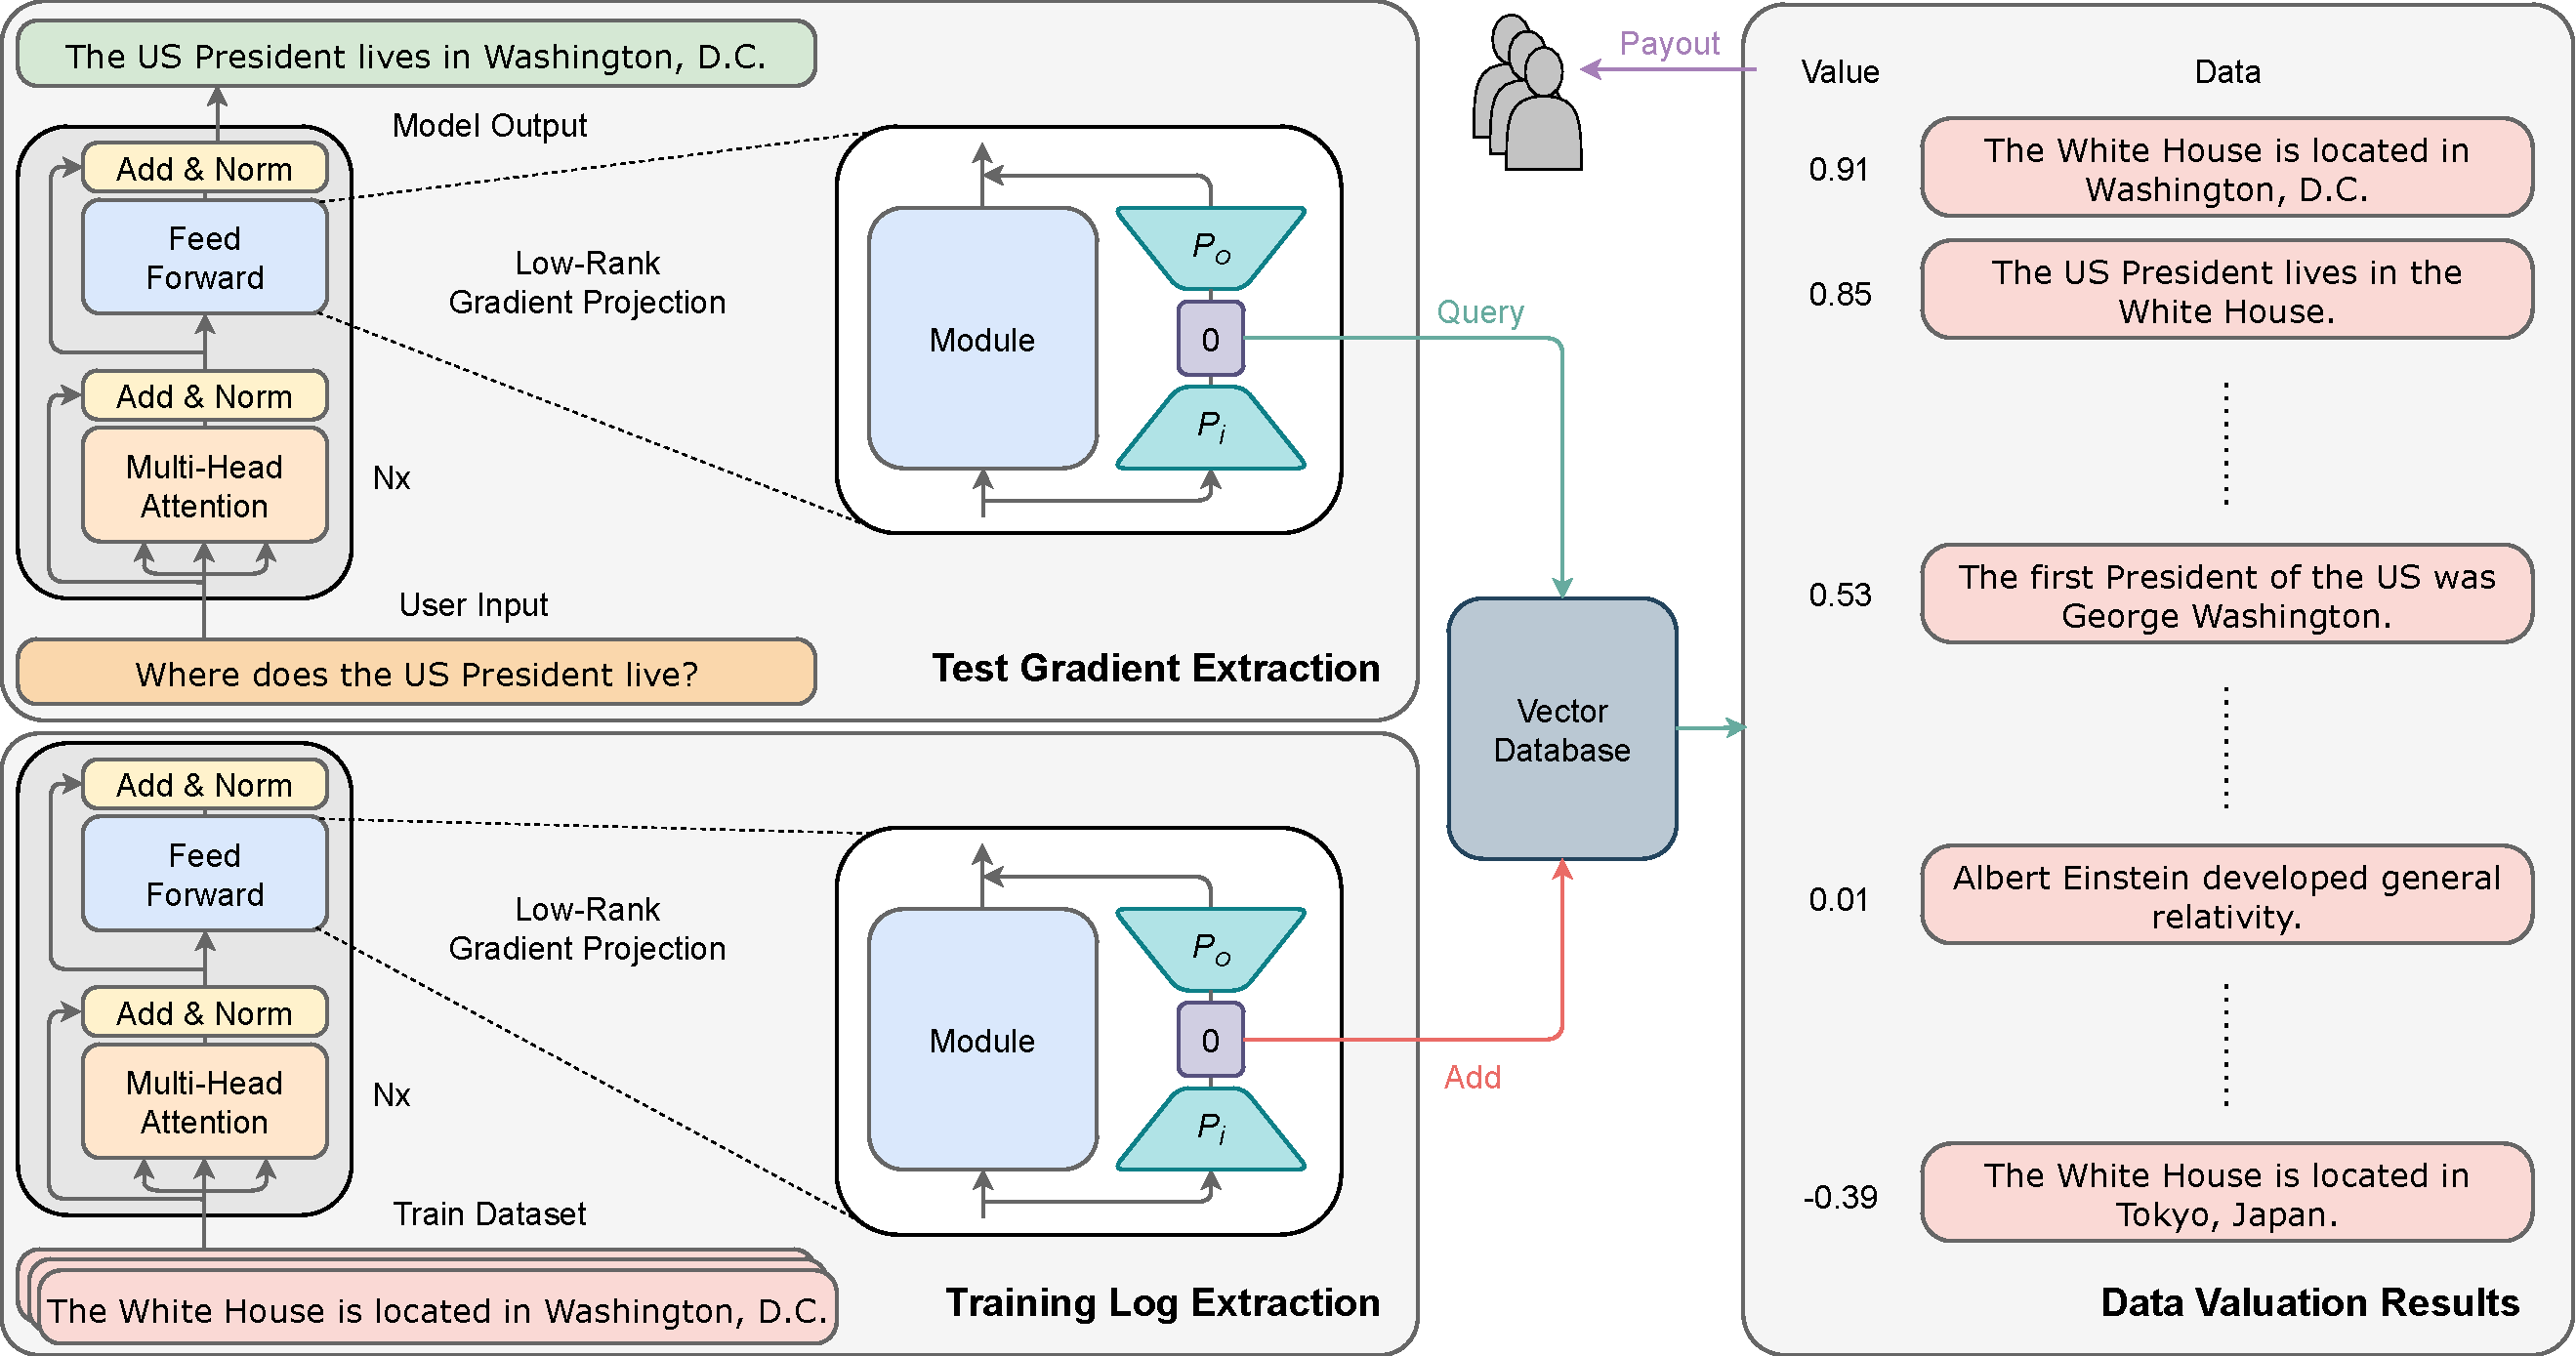
\includegraphics[width=0.94\textwidth]{figures/diagram_v7.pdf}
    \vskip -4pt
    \caption{Data valuation system architecture. \textbf{(Left Bottom)} We first extract the Hessian and gradients for all training data using efficient gradient projection \method\ and store them in a database. \textbf{(Left Top)} At test time, we similarly extract gradients and query the database. \textbf{(Right)} The database returns similarity scores with respect to training examples that can be used for data valuation/attribution.}
    \label{fig:diagram}
\end{figure}

\begin{itemize}[leftmargin=*,topsep=-2pt]
    \item Employing gradient structures in backpropagation, we develop a novel \textbf{lo}w-rank \textbf{gra}dient projection algorithm \method\ that improves space \& time complexity of gradient projection, a major scalability bottleneck in prior work~\cite{park2023trak,schioppa2022scaling}, from $O(nk)$ to $O(\sqrt{nk})$ where $n$ and $k$ are model and projection dimensions. Furthermore, \method\ directly computes projected gradients without materializing full gradients, enabling low GPU memory and high GPU utilization for improved efficiency. Lastly, we show that \method\ can be easily implemented with small add-on layers, similarly to LoRA~\cite{hu2021lora}.
    \item By interpreting a damping term in influence functions as a spectral gradient sparsification mechanism, we (1) offer a theoretical motivation of gradient projection approaches to influence functions and (2) derive a specialized PCA initialization scheme for \method.
    \item We introduce software named \software\ that (1) makes it \textit{simple} to convert existing training code into data valuation code, (2) is \textit{compatible} with various scalability tools and features in the LLM ecosystem, and (3) is \textit{extensible} to implement other data valuation or interpretability algorithms.
    \item In our data valuation experiments, \method\ demonstrates competitive accuracy against more costly baselines, while showing up to 6,500$\times$ increase in throughput and 5$\times$ reduction in GPU memory, when applied to Llama3-8B-Instruct~\cite{llama3modelcard} and the 1B-token dataset, compared to EKFAC influence \cite{grosse2023studying}, the state-of-the-art and only runnable baseline at this scale. We also observe that most valuable data identified by \method\ generally share qualitative similarities with the queried LLM output.
\end{itemize}
% Discuss preliminaries for time series modeling? 
\section{Preliminaries}
%
% Should also discuss two kinds of forecasting?  
% \begin{itemize}
%     \item Iterated multi-step forecasting (IMS): Recursive and direct multi-step forecasting: the best of both worlds, volume 19 
%     \item Direct multi-step (DMS): Direct multi-step estimation and forecasting.
% \end{itemize}
% \subsection{Problem Setting}

\header{Problem setting} We evaluate effective time series modeling with
% In this work, we evaluate effective time series modeling with accurate 
classification and forecasting tasks. For both tasks, we are given input sequences of $\ell$ ``look-back'' or ``lag'' time series samples $\boldsymbol{u}_{t - \ell: t - 1} = (u_{t - \ell}, \ldots, u_{t - 1}) \in \mathbb{R}^{\ell \times m}$ for sample feature size $m$. 
%
For classification, we aim to classify the sequence as the true class $y$ out of  possible classes $\mathcal{Y}$. 
For forecasting, we aim to correctly predict $H$ future time-steps over a ``horizon'' $\boldsymbol{y}_{t, t + h - 1} = (u_{t}, \ldots, u_{t + h - 1}) \in \mathbb{R}^{h \times m}$.
% To do so, we require methods that are both expressive and efficient.

% \subsection{State-Space Models for Time Series}
\header{State-space models for time series} 
We build on the discrete-time state-space model (SSM), which maps observed inputs $u_k$ to hidden states $x_k$, before projecting back to observed outputs $y_k$
\begin{align}
    x_{k+1} &= \zA x_k + \zB u_k  \label{eq:discrete_ssm_state} \\
    y_k &= \zC x_k + \zD u_k \label{eq:discrete_ssm_output}
\end{align}
where $\zA\in\R^{d\times d}$, $\zB\in\R^{d \times m}$, $\zC\in\R^{m' \times d}$, and $\zD\in\R^{m' \times m}$. 
% where $\zA\in\R^{d\times d}$, $\zB\in\R^{d \times m}$, $\zC\in\R^{m \times d}$, and $\zD\in\R^{m \times m}$. 
%
% The same relationship specified by $A, B, C, D$ holds for all samples in the input sequence $\boldsymbol{u}$ and output sequence $\boldsymbol{y}$. 
% To model time series in the \emph{single} SSM setting, because data is typically given as a single sequence, we treat $\boldsymbol{u}$ and $\boldsymbol{y}$ as copies of the same time series sequence. 
% To model time series in the \emph{single} SSM setting, we treat $\boldsymbol{u}$ and $\boldsymbol{y}$ as copies of the same time series sequence, such that
For now,  
% standard linear dynamical systems conventions, 
we stick to \emph{single-input single-output} conventions where $m, m' = 1$, and let $\zD = 0$. 
%
To model time series in the single SSM setting, we treat $\boldsymbol{u}$ and $\boldsymbol{y}$ as copies of the same process, such that  
% \st{}
% Matrices $A, B, C$ thus govern how the time series evolves over time as
% % We use the conventional linear dynamical systems (LDS) notation also adopted in prior work~\citep{Brogan:226422, gu2021combining}. 
\begin{equation}
    y_{k + 1} = u_{k + 1} = \zC(\zA x_k + \zB u_k)
\label{eq:input_output_ts_equal}
\end{equation}
We can thus learn a time series SSM by treating $\zA, \zB, \zC$ as black-box parameters in a neural net layer, \ie{} by updating $\zA, \zB, \zC$ via gradient descent \st{} with input $u_k$ and state $x_k$ at time-step $k$, following (\ref{eq:input_output_ts_equal}) predicts $\hat{y}_{k + 1}$ that matches the next time-step sample $y_{k + 1} = u_{k + 1}$.
%
This SSM framework and modeling setup is similar to prior works~\citep{gu2021combining, gu2021efficiently}, which adopt a similar interpretation of inputs and outputs being derived from the ``same'' process, \eg{} for language modeling. Here we study and improve this framework for time series modeling.
%
As extensions, in Sec.~\ref{sec:expressive_ssm_with_companion} we show how (\ref{eq:discrete_ssm_state}) and (\ref{eq:discrete_ssm_output}) express univariate time series with the right $\zA$ representation.
% and generalize to multivariate time series in Sec.~\ref{sec:method_architecture_overview}. 
%
In Sec.~\ref{sec:method_spacetime_layer} we discuss the multi-layer setting, where layer-specific $\boldsymbol{u}$ and $\boldsymbol{y}$ now differ, and we only model first layer inputs and last layer outputs as copies of the same time series process.
% In Sec.~\ref{todo}, we show how we learn a time series SSM by treating $\zA, B, C$ as black-box parameters in a linear neural network layer, \ie{} by updating $\zA, B, C$ via gradient descent \st{} with input $u_k$ and state $x_k$ at time-step $k$, (\ref{eq:input_output_ts_equal}) results in prediction $\hat{y}_{k + 1}$ that matches the next time-step sample $y_{k + 1} = u_{k + 1}$. 

% predicting future samples from past samples, and training the SSM with a regression objective between the predicted and ground-truth outputs.
% via supervised regression between predicted outputs $\hat{\boldsymbol{y}} = \text{SSM}(\zu)$ and $\zy$.

% While \cite{gu2021combining} also model the continuous version of (\ref{eq:discrete_ssm_state}, \ref{eq:discrete_ssm_output}), we stick with the discrete SSM due to its relative simplicity, alignment with how time series data is often a discrete sequence, and expressive power.
% %
% In the next section, we expand on this last point. We introduce our specific formulation of $\zA$ as the companion matrix, and show how this enables learning expressive SSMs for a wide range of time series processes (which are not all learnable via prior continuous SSMs). 

% \header{Expressiveness}


% \subsection{Core Challenges for Effective Time Series Modeling}

% \header{Expressiveness}
% \MZ{
% Describe how we need to be able to capture higher-order dependencies. Need large enough model dimension size to do this. For example, DLinear does lag input size times prediction size. 
% }

% \header{Efficiency}
% \MZ{
% Discuss how we want to get to $O(D + L)$, but the naive solution is $O(DL)$. Describe why this is important for time-series (in order to actually learn higher-order and long-range dependencies, we need large enough dimension size for the model, and need to be able to process long enough sequence, with reasonable time-frame and memory size.

% For example, DLinear does lag input size times prediction size. This is not great, because you end up with a very big model where model parameters scale with the size of the input sequence and the horizon.  

% It's also not very robust to different timesteps? But we are more robust? 


% }
\begin{figure}[t]
    \centering
    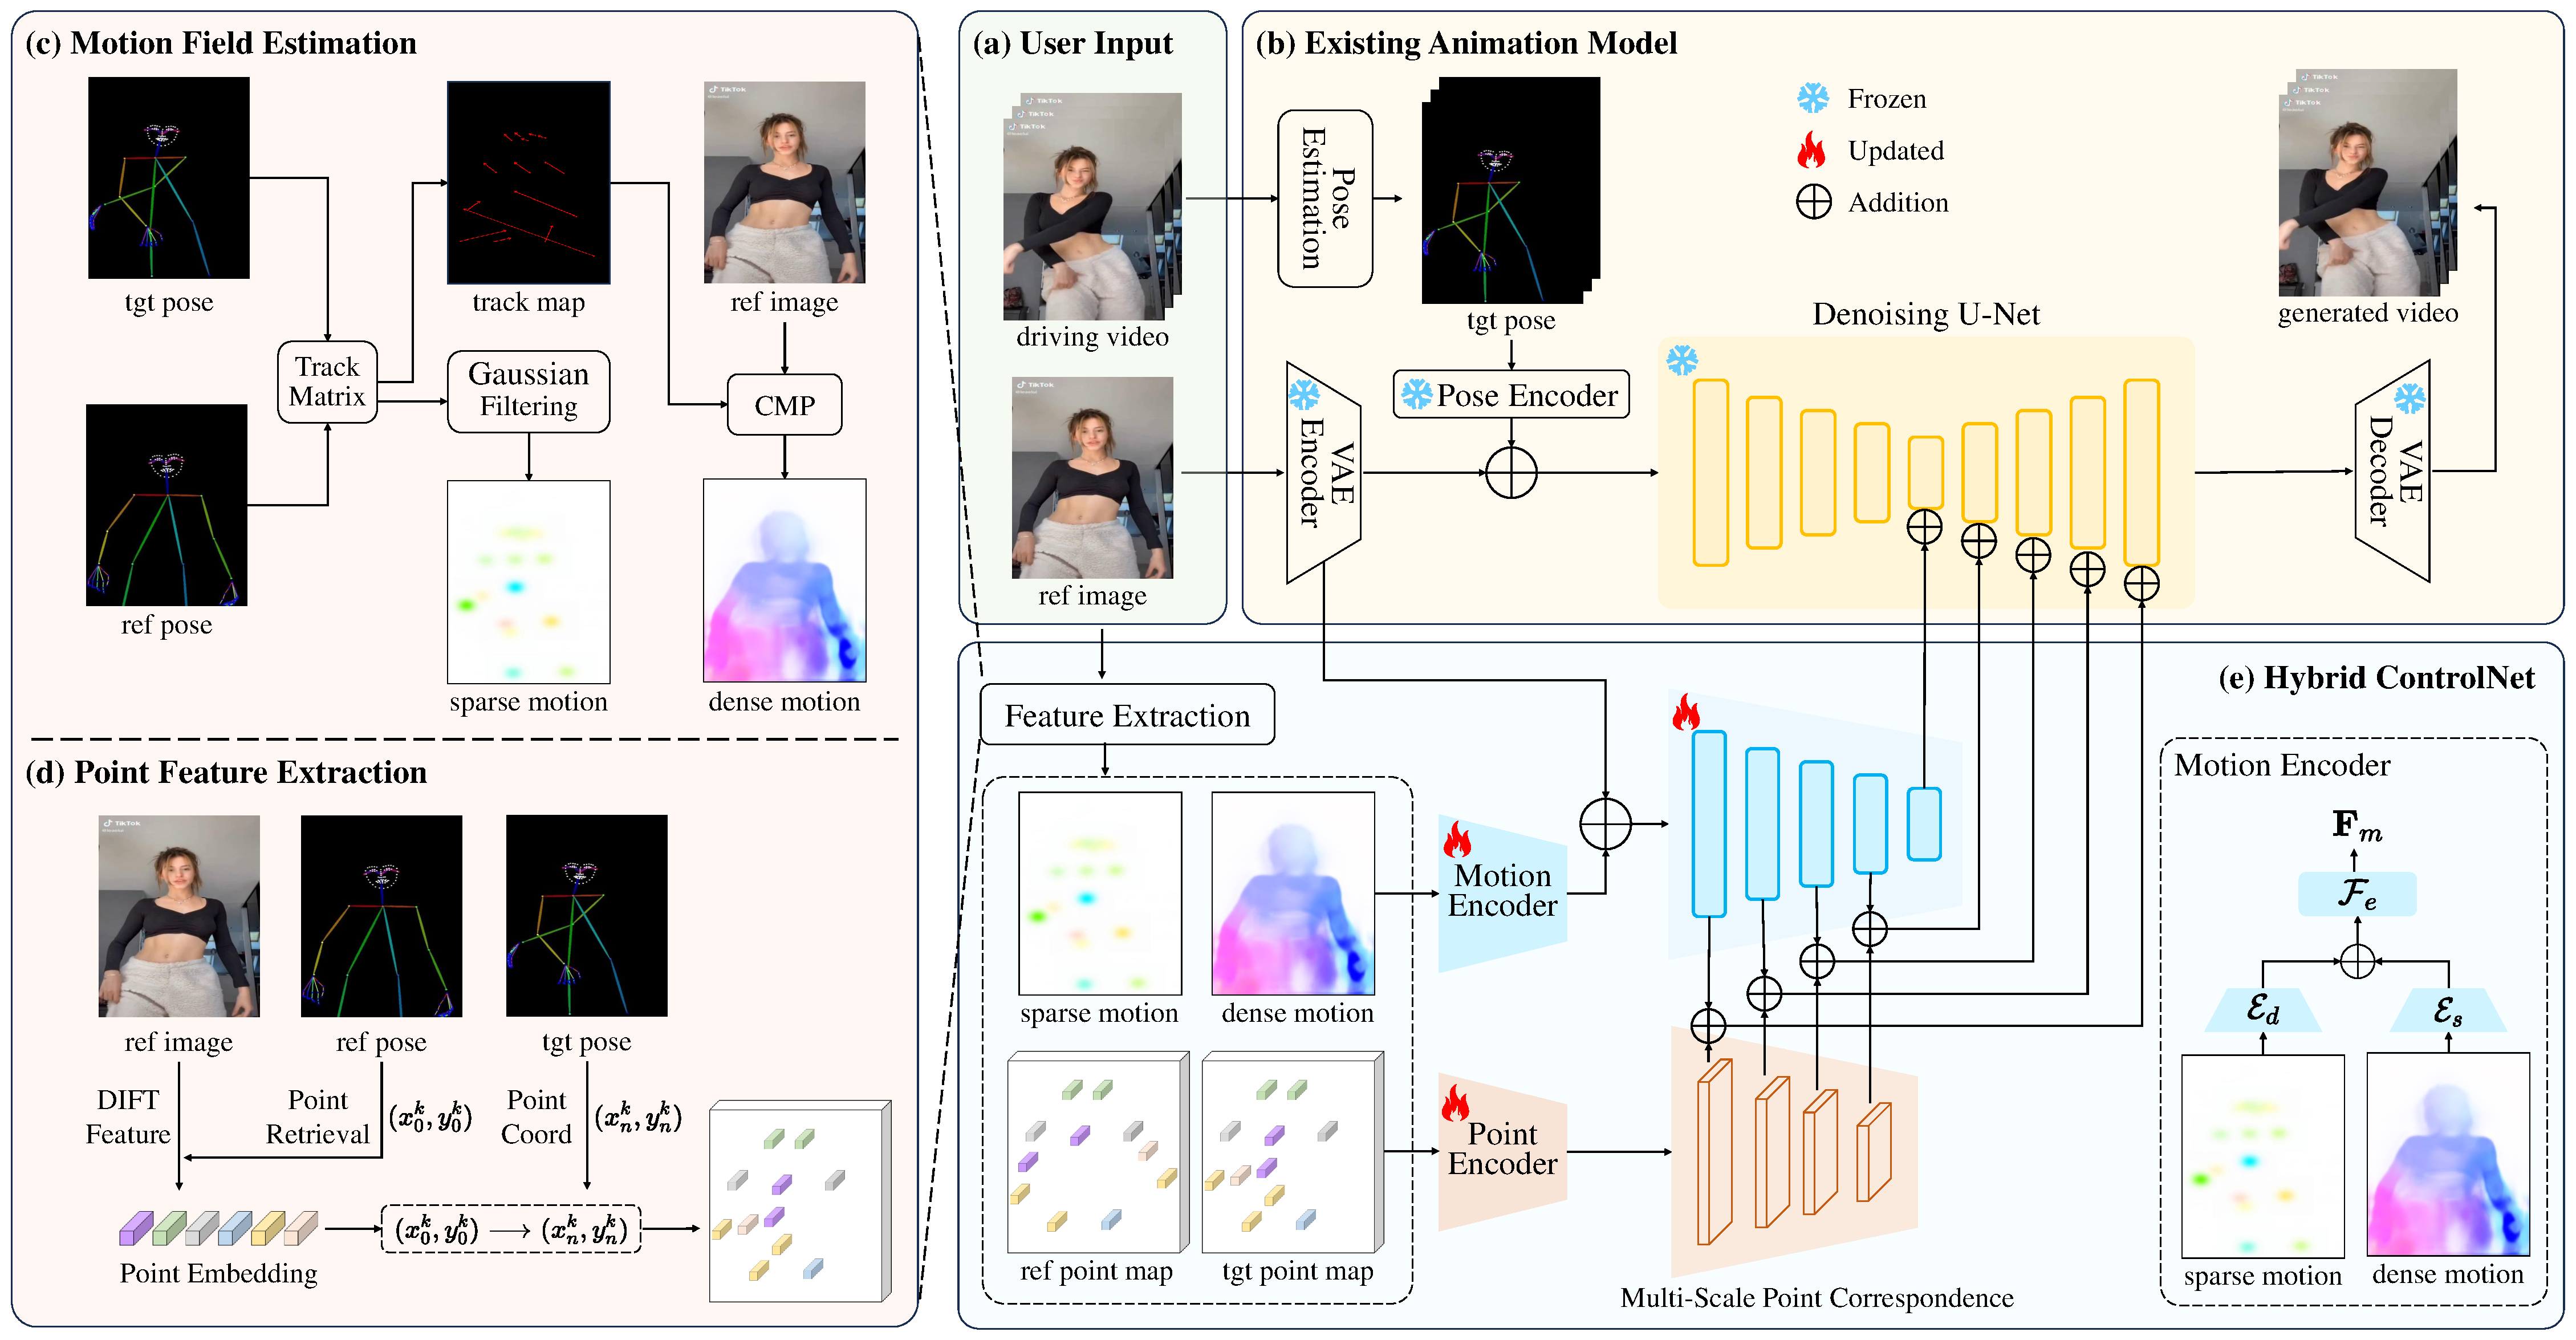
\includegraphics[width=1.0\columnwidth]{./image/pipeline.pdf}
    \vspace{-15pt}
    \caption{The overview of proposed DisPose.}
    \label{fig:pipeline}
\end{figure}
\section{DisPose}
Given a reference image $I_{\mathrm{ref}}\!\in\!\mathbb{R}^{3 \times H \times W}$ and a driving video $V\!\in\!\mathbb{R}^{N\times 3 \times H \times W}$. The core of our method is to disentangle efficient control guidance from only skeleton poses and reference images as shown in Figure~\ref{fig:pipeline}, which can be applied to existing human animation methods without additional dense inputs. We first introduce sparse and dense motion field guides in Sec.~\ref{sec: motion}. Then, we introduce reference-based keypoint correspondence in Sec.~\ref{sec: keypoint}. Finally, we introduce the pipeline of hybrid ControlNet in Sec~\ref{sec: controlnet}.
\subsection{Motion Field Guidance}
\label{sec: motion}

\textbf{Sparse Motion Field.}
We first estimate the skeleton pose by DWpose~\citep{yang2023dwpose} to obtain each frame's human key point coordinates. 
% Subsequently, the motion trajectory of all semantic points in the entire video is obtained and represented as
Subsequently, the key points of the reference image are used as starting points to track the motion displacement of all frames and represented as $P_{traj}\!=\!\{(x^k_n,y^k_n) \!\mid\! k=1\dots K, n=0\dots N\}$, where $P_{traj}$ denotes the trajectory map of the key point $k$ overall $N$ frames and $n = 0$ denotes the reference image. We calculate the track matrix $P_{s}$ as follows:
\begin{equation}
    \mathbf{P}_{s}=\{(x^k_n-x^k_{n-1}, y^k_n-y^k_{n-1}) \mid n=1\dots N\}\},
\end{equation}
% where $P_{t}$ denotes the trajectory map of the key point point $k$ over all $N$ frames, and the reference frame when $n = 0$.
where $K$ denotes the number of keypoints, $N$ denotes the number of frames, $\mathbf{P}_{s}$ denotes the trajectory map of keypoint k over all N frames, and $n = 0$ denotes the reference image.
To avoid training instability caused by overly sparse trajectory matrice, we then apply Gaussian filtering to enhance $\mathbf{P}_{s}$ to obtain the sparse motion field $\mathbf{F}_s\!\in\!\mathbb{R}^{(N-1)\times 2 \times H \times W}$ inspired by~\citep{yin2023dragnuwa, wang2024motionctrl}.

\textbf{Dense Motion Field.}
Considering that sparse control provides limited guidance and dense control is hard to obtain during inference,
% For the dense motion field, 
we transform dense guidance into the motion propagation from the reference frame to the target pose, instead of the dense signal of the target pose. Specifically, in the inference, we reconstruct the trajectory map $\mathbf{P}_{s}$ as the reference-based sparse optical flow $\mathbf{P}_{d}$ from the reference frame to each target pose as:
\begin{equation}
    \mathbf{P}_{d}=\{(x^k_n-x^k_{0}, y^k_n-y^k_{0}) \mid n=1\dots N\}\},
\end{equation}
We then predicted the reference-based dense motion filed $\mathbf{F}_d\!=\! \text{CMP}(P_{traj}, \mathbf{P}_{d}, I_{ref})\!\in\!\mathbb{R}^{(N-1)\times 2 \times H \times W}$ by condition motion propagation (CMP)~\citep{zhan2019self} based on the sparse optical flow $\mathbf{P}_{d}$ and the reference image $I_{ref}$.
CMP~\citep{zhan2019self} is a self-supervised learning-from-motion model that acquires an image and a sparse motion field and estimates the corresponding dense motion field.
Notably, the dense motion field $\mathbf{F}_d$ of each frame starts with the reference image, which avoids geometric constraints during inference.

To ensure motion estimation accuracy during training, we first extract the forward optical flow from the driving video using existing optical flow estimation models~\citep{teed2020raft, xu2023unifying}. We then use a watershed-based approach~\citep{zhan2019self} to sample the sparse optical flow $\mathbf{P}_{d}$ from the forward optical flow. See Appendix.~\ref{sec: appendix1} for details.

\textbf{Motion Encoder.} To leverage motion field as guidance, we introduce a motion encoder specifically designed for the optional flow, which includes sparse motion encoder $\mathcal{E}_s$, dense motion encoder $\mathcal{E}_d$ and feature fusion layer $\mathcal{F}_e$. $\mathcal{E}_d$ and $\mathcal{E}_s$ have the same structure and are multi-scale convolutional encoders with each stage built by \texttt{Conv-SiLU-ZeroConv}~\citep{zhang2023adding} as the basic block. The feature fusion layer $\mathcal{F}_e$ is a 2D convolution for fusing sparse motion features $\mathcal{E}_s(\mathbf{F}_s)$ and dense motion features $\mathcal{E}_d(\mathbf{F}_d)$. Finally, we compute the motion field guidance $\mathbf{F}_m$:
\begin{equation}
    \mathbf{F}_m = \mathcal{F}_e(\mathcal{E}_s(\mathbf{F}_s)+\mathcal{E}_d(\mathbf{F}_d))
\end{equation}

\subsection{Keypoint Correspondence}
\label{sec: keypoint}
\textbf{Point Feature Extraction.} 
To maintain a consistent appearance, it is crucial to correspond the content of the reference image with the motion trajectory. 
Specifically, we first extract the DIFT~\citep{tang2023emergent} features $\mathbf{D}$ of the reference image using the pre-trained image diffusion model. 

Subsequently, the keypoint embedding in the reference is obtained as $\mathbf{D}(x^k_0,y^k_0)$, where $(x^k_0,y^k_0)$ is retrieved from the reference pose.
% key point embeddings $\mathbf{D}(x^k_0,y^k_0)$ are retrieved from $\mathbf{D}$ by skeleton pose $(x^k_0, y^k_0)$.
Next, we initialize the keypoint correspondence map $\mathbf{F}_p$ with zero vectors and assign point embeddings according to the trajectory coordinates as:
\begin{equation}
\label{eq: v prob}
f^{ij}_n=\left\{\begin{array}{ll}
\mathbf{D}(x^k_0,y^k_0), & \mathrm{if} \quad i=x^k_n, j=y^k_n,  \\
0, & \mathrm{otherwise}.
\end{array}\right.
\end{equation}

Finally, we obtain the keypoint correspondence map $\mathbf{F}_p=\{f_n\!\mid\!n=1\dots N\} \!\in\!\mathbb{R}^{N\times D_p \times H \times W}$ for all frames, where $D_p$ is the feature dimension of the point embedding.

\textbf{Point Encoder.} 
To utilize the content correspondence of key points as guidance, we generate multi-scale correspondences of sparse point feature maps and make them compatible with the U-Net encoder of the {Hybrid ControlNet (Sec.4.3)}. 
% as detailed in F. 1.
We introduce the multi-scale point encoder $\mathcal{E}_p$ to maintain the key point content $\mathbf{F}_p$ from the reference image. The point encoder $\mathcal{E}_p$ consists of a series of learnable MLPs.
{
To seamlessly integrate into existing models, we extract intermediate features of the encoder of the hybrid Controlnet.
The multi-scale intermediate features of the Controlnet encoder are denoted as $\mathbf{E}^l_{enc}$, where $l$ denotes each U-Net block $l\!\in\![1, L]$.}
To match the spatial size of $\mathbf{E}^l_{enc}$, we apply downsampling to the feature map between the encoder layers. We compute the multi-scale keypoint correspondence as follows:
\begin{equation}
    \mathbf{F}_c^l = \mathcal{E}_p^l(\phi(\mathbf{F}_p, H^l, W^l)),
\end{equation}
where $(H^l, W^l)$ are denote the spatial dimension of the $l$-th U-Net block and $\phi$ means downsampling operation. Therefore, $\mathbf{F}_c^l$ shares the same size as $\mathbf{E}^l_{enc}$.
Finally, $\mathbf{F}_c$ are added elementwisely to the intermediate feature $\mathbf{E}^l_{enc}$ of the U-Net encoder as guidance: $\mathbf{E}^l_{enc}\!=\!\mathbf{E}^l_{enc}+\mathbf{F}_c^l$.


\subsection{Plug-and-play Hybrid ControlNet}
\label{sec: controlnet}
After obtaining motion field guidance and keypoint correspondence, we aim to integrate these control guidance seamlessly into the U-Net architecture of existing animation models.
Inspired by ControlNet~\citep{zhang2023adding}, We design a hybrid ControlNet $\mathcal{F}$ to provide additional control signals for the existing animation model as shown in Figure~\ref{fig:pipeline}(e).
% Specifically, we consider freeze denoising U-Net and pose encoder. 
Specifically, given an animation diffusion model based on the U-Net architecture, we freeze all its modules while allowing the motion encoder, point encoder and hybrid ControlNet to be updated during training. 
Subsequently, $\mathbf{F}_m$ is added to the noise latent before being input into the hybrid ControlNet. Considering the high sparsity of the point feature $\mathbf{F}_c$, we correspondingly add $\mathbf{F}_c$ to the input of the convolutional layer. Notably, the U-Net encoder intermediate feature $\mathbf{E}_{enc}$ in Sec.~\ref{sec: keypoint} is from hybrid ControlNet rather than denoising U-Net. Finally, 
the control condition is computed as:
\begin{equation}
    \boldsymbol{r}=\mathcal{F}(\boldsymbol{z}_{{t}} \mid \mathbf{F}_m, \mathbf{F}_c, {t})
\end{equation}
where $\boldsymbol{r}$ is a set of condition residuals added to the residuals for the middle and upsampling blocks in the denoising U-Net.
\section{Experiments}
\label{sec:experiments}

We validate our approach empirically, showing that our Monarch matrix parametrization achieves a favorable efficiency--accuracy tradeoff compared to baselines on a wide range of domains (text, images, PDEs, MRI), in three settings (E2E training, S2D training, and D2S fine-tuning):
\begin{itemize}[leftmargin=*,nosep,nolistsep,noitemsep]
\item
In \cref{subsec:benchmark_tasks}, on image classification and language modeling benchmarks, such as ViT / MLP Mixer on ImageNet and GPT-2 on Wikitext-103, Monarch is 2$\times$ faster to train than dense models, while achieving the same accuracy / perplexity. In \cref{subsec:pde_mri}, in scientific and medical domains where special transforms (Fourier) are common, Monarch outperforms Fourier transform based methods on PDE solving, with up to 40\% lower error, and on MRI reconstruction attains up to 15\% higher pSNR and 3.8\% higher SSIM.
\item In \cref{subsec:pde_mri}, we show that on the large OpenWebText dataset, reverse sparsification (training with Monarch weight matrices for most of the time, then transitioning to dense weight matrices) speeds up the pretraining of GPT-2 models by 2$\times$ compared to the dense model, with no loss in upstream or downstream quality.
Moreover, reverse sparsification speeds up BERT pretraining by 23\% even compared to the implementation from Nvidia that set the MLPerf~\citep{mattson2020mlperf} 1.1 record.
\item In \cref{subsec:finetuning}, as a proof of concept, we demonstrate that our Monarch approximation algorithm can improve fine-tuning efficiency for pretrained models. We show that compressing BERT to a Monarch matrix model performs comparably to a finetuned dense model on GLUE, with 2$\times$ fewer parameters and 1.7$\times$ faster finetuning speed.
\end{itemize}

\subsection{End-to-End Training}
\label{subsec:e2e_training}
\subsubsection{Benchmark Tasks: Image Classification, Language Modeling}
\label{subsec:benchmark_tasks}

We show that replacing dense matrices with Monarch matrices in ViT, MLP-Mixer, and
GPT-2 can speed up training by up to 2$\times$ without sacrificing model quality in~\cref{table:pretrain,table:gpt_pretrain}.

\textbf{Setup.} We use the popular vision benchmark, ImageNet~\citep{deng2009imagenet}. We choose recent popular Vision Transformer~\citep{dosovitskiy2020image}, and MLP-Mixer~\citep{tolstikhin2021mlp} as representative base dense models.
For language modeling, we evaluate GPT-2~\citep{radford2019language} on WikiText-103~\citep{merity2016pointer}.

\begin{table}[h]
  \small
  \centering
  \vspace{-2mm}
  \caption{\label{table:pretrain}The performance of Monarch matrices and ViT / MLP-Mixer on ImageNet, including the number of parameters and FLOPs. We measure the Top-1 accuracy and the training time speedup compared to the corresponding dense model. %
  \vspace{2mm}
  }
  \iftoggle{arxiv}{}{
  \resizebox{\linewidth}{!}
  }
  {
  \setlength{\tabcolsep}{3pt}
  \vspace{3em}
  \begin{tabular}{@{}c||ccccccc@{}}
  \specialrule{.15em}{.05em}{.05em}
    Model&\multicolumn{1}{c}{ImageNet acc.}&\multicolumn{1}{c}{Speedup} &\multicolumn{1}{c}{Params} & \multicolumn{1}{c}{FLOPs} \\
    \specialrule{.15em}{.05em}{.05em}
    Mixer-S/16& 74.0& - & 18.5M & 3.8G \\
    Monarch-Mixer-S/16& 73.7& 1.7$\times$ & 7.0M & 1.5G \\
    Mixer-B/16& 77.7& - & 59.9M & 12.6G \\
    Monarch-Mixer-B/16& 77.8& 1.9$\times$ & 20.9M & 5.0G \\
    \specialrule{.15em}{.05em}{.05em}
    ViT-S/16& 79.4 & - & 48.8M & 9.9G \\
    Monarch-ViT-S/16& 79.1 & 1.9$\times$ & 19.6M & 3.9G \\
    ViT-B/16& 78.5 & - & 86.6M  & 17.6G \\
    Monarch-ViT-B/16& 78.9 & 2.0$\times$ & 33.0M & 5.9G \\
    \specialrule{.15em}{.05em}{.05em}
  \end{tabular}
  }
\end{table}

\begin{table}[h]
  \small
  \centering
  \vspace{-3mm}
  \caption{\label{table:gpt_pretrain} Performance of Monarch matrices and GPT-2-Small/Medium on WikiText-103, including the \# of parameters and FLOPs. Monarch achieves similar perplexity (ppl) but 2.0$\times$ faster.}
  \vspace{1mm}
  \iftoggle{arxiv}{}{
    \resizebox{0.95\linewidth}{!}
  }
  {
\setlength{\tabcolsep}{5pt}
\begin{tabular}{c||cccc}
\specialrule{.15em}{.05em}{.05em}
\multirow{1}{*}{{ Model} } & \multicolumn{1}{c}{\multirow{1}{*}{PPL}}
                              & \multicolumn{1}{c}{\multirow{1}{*}{Speedup}}
                              & \multicolumn{1}{c}{\multirow{1}{*}{Params}}
                              & \multicolumn{1}{c}{\multirow{1}{*}{FLOPs}}\\
\specialrule{.15em}{.05em}{.05em}
GPT-2-Small &  20.6 & - & 124M& 106G\\
Monarch-GPT-2-Small& 20.7  & 1.8$\times$ &72M & 51G\\
\specialrule{.15em}{.05em}{.05em}
GPT-2-Medium &  20.9 & - & 355M& 361G\\
Monarch-GPT-2-Medium& 20.3  & 2.0$\times$ &165M & 166G\\
\specialrule{.15em}{.05em}{.05em}
\end{tabular}
}
\vspace{-2mm}
\end{table}


\subsubsection{PDE solving and multi-coil MRI reconstruction}
\label{subsec:pde_mri}

Many scientific or medical imaging tasks rely on specialized transforms such as the
Fourier transform.
We show that replacing the fixed Fourier transform with the more expressive
Monarch matrices yields higher model quality (lower reconstruction error) with
comparable model speed.

\textbf{Solving PDEs with Monarch Neural Operators.}
We follow the experimental setting in FNO~\citep{li2020fourier} and apply a Monarch--based neural operator to the task of solving the Navier--Stokes PDE. Compared to baseline U-Nets~\citep{ronneberger2015u}, TF-Nets~\citep{wang2020towards}, ResNets~\citep{he2016deep} and FNOs~\cite{li2020fourier}, neural operators based on Monarch improve solution accuracy across spatial resolutions by up to $40\%$ (Table \ref{table:pde}).  





\paragraph{Non-periodic boundary conditions.} Traditional spectral methods based on Fourier transform work best with periodic boundary conditions and forcing terms. However, PDEs of practical interest often exhibit non--periodic or even unknown boundary conditions. Monarch operators are not constrained to the Fourier transform and can thus still learn the solution operator with excellent accuracy.

\begin{table}[h!] 
\scriptsize
\vspace{-4mm}
\caption{\label{table:pde}Benchmarks on Navier-Stokes (fixing resolution 64 × 64 for both training and testing).
Decreasing the viscosity coefficient $\nu$ makes the dynamics more chaotic.
}
\vspace{1mm}
\centering
\iftoggle{arxiv}{}{
  \resizebox{0.9\linewidth}{!}
}
{
\renewcommand{\arraystretch}{1}
\begin{tabular}{ c||ccc }
\specialrule{.15em}{.05em}{.05em}
Model & $v = 10^{-3}$  &  $v = 10^{-4}$ & $v = 10^{-5}$\\
\specialrule{.15em}{.05em}{.05em}
U-Net & 0.025  & 0.205  &   0.198\\
TF-Net  & 0.023  & 0.225 &  0.227 \\
ResNet & 0.070 &  0.287 &  0.275 \\
FNO & 0.017  & 0.178 & 0.155\\
Monarch-NO & \textbf{0.010} & \textbf{0.145} & \textbf{0.136} \\
\specialrule{.15em}{.05em}{.05em}
\end{tabular}
}
\textbf{\vspace{-3mm}}
\end{table}

\textbf{Accelerated MRI Reconstruction.} We characterize the utility of Monarch-based FFT operations for accelerated MRI reconstruction, a task which requires methods with both structured Fourier operators and dealiasing properties to recover high quality images. On the clinically-acquired 3D MRI SKM-TEA dataset \citep{desai2021skm}, Monarch-SENSE (mSENSE) enhances image quality by over 1.5dB pSNR and 2.5\% SSIM compared to zero-filled SENSE and up to 4.4dB and 3.8\% SSIM compared to U-Net baselines in data-limited settings. Setup details are available in~\cref{sec:experiment_details_mri}.

\paragraph{Expressive FFT.} By definition, standard IFFT in zero-filled SENSE cannot dealias the signal, resulting in artifacts in the reconstructed image. mSENSE replaces the inverse FFT (IFFT) operation in standard SENSE with learnable Monarch matrices. Thus, mSENSE preserves the structure of the Fourier transform while learning to reweight frequencies to suppress aliasing artifacts. Across multiple accelerations, mSENSE achieved up to +1.5dB and 2.5\% improvement in peak signal-to-noise ratio (pSNR) and structural similarity (SSIM), respectively (Table~\ref{table:mri}).

\paragraph{Data Efficiency.} While CNNs have shown promise for MRI reconstruction tasks, training these networks requires extensive amounts of labeled data to avoid overfitting. However, large data corpora are difficult to acquire in practice. mSENSE can be trained efficiently with limited supervised examples. In few shot settings, mSENSE can outperform U-Net by +4.4dB ($\approx$15\%) and 3.8\% SSIM (Table~\ref{table:mri-data-limited}). 







\begin{table}[h!] 
\scriptsize
\vspace{-3mm}
\caption{\label{table:mri}Mean $\pm$ standard error of the mean of conventional and Monarch-SENSE (mSENSE) on dual-echo (E1,E2) MRI reconstruction at multiple acceleration factors (Acc.).
}
\vspace{1mm}
\centering
\iftoggle{arxiv}{}{
  \resizebox{\linewidth}{!}
}
{
\renewcommand{\arraystretch}{1.2}
\begin{tabular}{c||ccccc}
\specialrule{.15em}{.05em}{.05em}
  & & \multicolumn{2}{c}{pSNR (dB) ($\uparrow$)} & \multicolumn{2}{c}{SSIM ($\uparrow$)} \\
  Acc. & Model &             E1 &             E2 &                E1 &                E2 \\
\specialrule{.15em}{.05em}{.05em}
\multirow{2}{*}{2} & SENSE &  32.8$\pm$0.2 &  35.4$\pm$0.2 &  0.871$\pm$0.003 &  0.865$\pm$0.003 \\
  & mSENSE &  \textbf{34.3$\pm$0.2} &  \textbf{36.6$\pm$0.2} &  \textbf{0.886$\pm$0.002} &  \textbf{0.882$\pm$0.003} \\
\specialrule{.15em}{.05em}{.05em}
\multirow{2}{*}{3} & SENSE &  30.9$\pm$0.2 &  33.5$\pm$0.2 &  0.819$\pm$0.004 &  0.795$\pm$0.004 \\
  & mSENSE &  \textbf{32.3$\pm$0.2} &  \textbf{34.6$\pm$0.2} &  \textbf{0.843$\pm$0.003} &  \textbf{0.820$\pm$0.004} \\
\specialrule{.15em}{.05em}{.05em}
\multirow{2}{*}{4} & SENSE &  30.1$\pm$0.2 &  32.8$\pm$0.2 &  0.789$\pm$0.004 &  0.753$\pm$0.005 \\
  & mSENSE &  \textbf{31.2$\pm$0.2} &  \textbf{33.5$\pm$0.2} &  \textbf{0.812$\pm$0.003} &  \textbf{0.767$\pm$0.005} \\
\specialrule{.15em}{.05em}{.05em}
\end{tabular}
}
\end{table}

\begin{table}[h!] 
\scriptsize
\vspace{-5mm}
\caption{\label{table:mri-data-limited}Impact of number of training examples ($N$) on dual-echo MRI reconstruction at 2x acceleration.
}
\vspace{1mm}
\centering
\iftoggle{arxiv}{}{
  \resizebox{\linewidth}{!}
}
{
\renewcommand{\arraystretch}{1.2}
\begin{tabular}{c||ccccc}
\specialrule{.15em}{.05em}{.05em}
  &  & \multicolumn{2}{c}{pSNR (dB) ($\uparrow$)} & \multicolumn{2}{c}{SSIM ($\uparrow$)} \\
  $N$ & Model &            E1 &            E2 &               E1 &               E2 \\
\specialrule{.15em}{.05em}{.05em}
N/A & SENSE &  32.8$\pm$0.2 &  35.4$\pm$0.2 &  0.871$\pm$0.003 &  0.865$\pm$0.003 \\
\specialrule{.15em}{.05em}{.05em}
\multirow{2}{*}{1} & U-Net &  29.4$\pm$0.2 &  34.4$\pm$0.3 &  0.848$\pm$0.004 &  0.857$\pm$0.004 \\
  & mSENSE &  \textbf{33.8$\pm$0.2} &  \textbf{36.0$\pm$0.2} &  \textbf{0.886$\pm$0.003} &  \textbf{0.867$\pm$0.003} \\
\specialrule{.15em}{.05em}{.05em}
\multirow{2}{*}{2} & U-Net &  29.9$\pm$0.3 &  35.1$\pm$0.3 &  0.858$\pm$0.003 &  0.871$\pm$0.003 \\
  & mSENSE &  \textbf{34.0$\pm$0.2} &  \textbf{36.4$\pm$0.2} &  \textbf{0.883$\pm$0.002} &  \textbf{0.877$\pm$0.003} \\
\specialrule{.15em}{.05em}{.05em}
\multirow{2}{*}{3} & U-Net &  31.0$\pm$0.3 &  35.2$\pm$0.3 &  0.866$\pm$0.003 &  0.867$\pm$0.004 \\
  & mSENSE &  \textbf{33.9$\pm$0.2} & \textbf{ 36.5$\pm$0.2} &  \textbf{0.882$\pm$0.002} & \textbf{0.878$\pm$0.003} \\
\specialrule{.15em}{.05em}{.05em}
\multirow{2}{*}{5} & U-Net &  31.4$\pm$0.3 &  35.6$\pm$0.2 &  0.877$\pm$0.002 &  0.870$\pm$0.003 \\
  & mSENSE &  \textbf{33.9$\pm$0.2} &  \textbf{36.5$\pm$0.2} &  \textbf{0.881$\pm$0.002} &  \textbf{0.877$\pm$0.003} \\
\specialrule{.15em}{.05em}{.05em}
\end{tabular}
}
\end{table}




\subsection{Sparse-to-Dense Training (reverse sparsification)}
\label{subsec:s2d_training}
\paragraph{GPT-2 pretraining.}
On the large OpenWebtext dataset~\citep{Gokaslan2019OpenWeb}, we train a GPT-2 model with Monarch weight
matrices for 90\% of the training iterations, then relax the constraint on the
weight matrices and train them as dense matrices for the remaining 10\% of the
iterations.
We call this technique ``reverse sparsification.''
Previous sparse training techniques often don't speed up training, whereas our
hardware-efficient Monarch matrices do.
Therefore we can use them as an intermediate step to pretrain a large language
model (GPT-2) in 2$\times$ less time. We also evaluate its downstream quality on zero-shot generation from~\citep{eval-harness} and classification tasks from~\citep{zhao2021calibrate}, achieving comparable performance to the dense counterparts (\cref{table:gpt_finetune}). 

\begin{table}[h]
  \small
  \centering
  \vspace{-3mm}
  \caption{\label{table:gpt_finetune}The performance (accuracy) of GPT-2-medium trained with Monarch reverse sparsification and with conventional dense training on text classification benchmarks.}
  \setlength{\tabcolsep}{5pt}
  \vspace{1em}
  \iftoggle{arxiv}{}{
    \resizebox{\linewidth}{!}
  }
  {
  \begin{tabular}{@{}c||ccc@{}}
    \specialrule{.15em}{.05em}{.05em}
    Model&\multicolumn{1}{c}{OpenWebText (ppl)}&\multicolumn{1}{c}{Speedup}& \multicolumn{1}{c}{Classification (avg acc)} \\
    \specialrule{.15em}{.05em}{.05em}
    GPT-2m& 18.0 & - & 38.9 \\
    Monarch-GPT-2m& 18.0 & 2$\times$ & 38.8 \\
    \specialrule{.15em}{.05em}{.05em}
  \end{tabular}
  }
  \vspace{-3mm}
\end{table}


In \cref{fig:reverse_sparsification_bar}, we show the training time of the dense GPT-2 model, along with
the Monarch GPT-2 model.
After training the Monarch model for 90\% of the time, in the
last 10\% of the training steps, by transitioning to dense weight matrices, the model is able to reach the same 
performance of another model that was trained with dense weight matrices from
scratch.
By training with Monarch matrices for 90\% of the time, we reduce the total training time by 2$\times$.

\paragraph{BERT pretraining.}
On the Wikipedia + BookCorpus datasets~\citep{zhu2015aligning}, we train a BERT-large model with Monarch weight matrices for 70\% of the time and transition to dense weight matrices for the remaining 30\% of the time, which yields the same pretraining loss as conventional dense training.
In \cref{table:bert_speed}, we compare the total training time to several baseline implementations: the widely-used implementation from HuggingFace~\citep{wolf-etal-2020-transformers}, the more optimized implementation from Megatron~\citep{shoeybi2019megatron}, and the most optimized implementation we know of from Nvidia that was used to set MLPerf 1.1 training speed record. Our method is 3.5x faster than HuggingFace and 23\% faster than Nvidia's MLPerf 1.1 implementation\footnote{Our result is not an official MLPerf submission. We train BERT for both phase 1 (sequence length 128) and phase 2 (sequence length 512) according to the standard BERT training recipe\cite{devlin2018bert}, while MLPerf only measures training time for phase 2.}.
Experiment details are in~\cref{subsec:bert_details}.

\begin{table}[h]
  \small
  \centering
  \caption{\label{table:bert_speed}The total training time of BERT-large trained with Monarch reverse sparsification and with conventional dense training on 8 A100-40GB GPUs (DGX A100). Training consists of two phases, phase 1 with sequence length 128 and phase 2 with sequence length 512. Monarch training is 3.5x faster than HuggingFace and 23\% faster than Nvidia's MLPerf 1.1 implementation.}
  \vspace{1em}
  \iftoggle{arxiv}{}{
    \resizebox{\linewidth}{!}
  }
  {
    \begin{tabular}{@{}c||c@{}}
      Implementation & Training time (h)  \\ \hline
      HuggingFace &  84.5 \\
      MegaTron & 52.5 \\
      Nvidia MLPerf 1.1 & 30.2 \\
      Nvidia MLPerf 1.1 + DeepSpeed & 29.3 \\
      Monarch (ours) & \textbf{23.8} \\
    \end{tabular}
  }
  \vspace{-3mm}
\end{table}

\subsection{Dense-to-Sparse Fine-tuning}
\label{subsec:finetuning}

\begin{figure}[t]
  \centering
  \vspace{-3mm}
  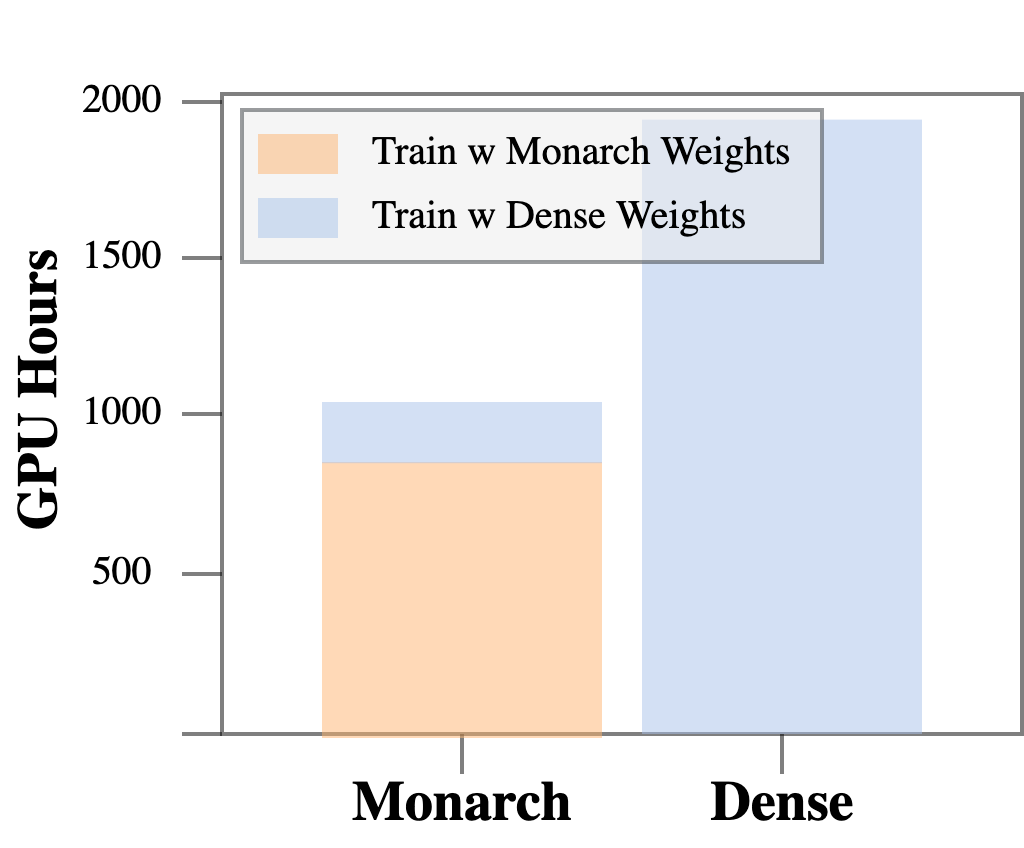
\includegraphics[width=.3\textwidth]{figures/rv_bar_temp.png}
  \vspace{-3mm}
  \caption{\label{fig:reverse_sparsification_bar}Time required (in A100 GPU hours) to reach the same perplexity (18.0)
    for GPT-2-small on OpenWebText.
    With ``reverse sparsification'', Monarch can speed up
    GPT-2 training by 2$\times$.\vspace{-1em}}
\end{figure}

We show that our Monarch approximation algorithm allows us to efficiently use
pretrained models, such as speeding up BERT finetuning on GLUE.

\paragraph{BERT finetuning.}
We take the BERT pretrained weights, approximate them with Monarch matrices,
and finetune the resulting model on the 9 GLUE tasks.
The results in \cref{table:bert_glue} shows that we obtain a Monarch finetuned
model with similar quality to the dense BERT model, but with 1.7$\times$ faster
finetuning speed.
This serves as a proof of concept, and we expect further speedup if additional model compression techniques are applied (e.g., quantization, kernel fusion).




\begin{table}[h]
  \small
  \centering
  \vspace{-5mm}
  \caption{\label{table:bert_glue}The performance of Monarch matrices in
    finetuning BERT on GLUE.}
  \setlength{\tabcolsep}{5pt}
  \vspace{1em}
  \iftoggle{arxiv}{}{
    \resizebox{\linewidth}{!}
  }
  {
  \begin{tabular}{@{}c||ccccccc@{}}
  \specialrule{.15em}{.05em}{.05em}
    Model&\multicolumn{1}{c}{GLUE (avg)}&\multicolumn{1}{c}{Speedup} &\multicolumn{1}{c}{Params} & \multicolumn{1}{c}{FLOPs} \\
    \specialrule{.15em}{.05em}{.05em}
    BERT-base & 78.6& - & 109M & 11.2G \\
    Monarch-BERT-base& 78.3& 1.5$\times$ & 55M & 6.2G  \\
    BERT-large & 80.4 & - & 335M & 39.5G \\
    Monarch-BERT-large & 79.6 & 1.7$\times$ & 144M & 14.6G  \\
    \specialrule{.15em}{.05em}{.05em}
  \end{tabular}
  }
  \vspace{-3mm}
\end{table}




Hyperbolic embeddings embed hierarchical information with high
fidelity and few dimensions. We explored the limits of this approach
by describing scalable, high quality algorithms. We hope the
techniques here encourage more follow-on work on the exciting
techniques of \citet{fb, ucl}. As future work, we hope to explore how
hyperbolic embeddings can be most effectively incorporated into downstream
tasks and applications.


\newpage

\section{Ethics Statement}
A main objective of our work is to improve the ability to classify and forecast time series, which has real-world applications in many fields. These applications may have high stakes, such as classifying abnormalities in medical time series. In these situations, incorrect predictions may lead to harmful patient outcomes. It is thus critical to understand that while we aim to improve time series modeling towards these applications, we do not solve these problems. Further analysis and development into where models fail in time series modeling is necessary, including potentials intersections with research directions such as robustness and model biases when aiming to deploy machine learning models in real world applications.  
% 
% In many applications, such as classifying abnormal medical time series, incorrect predictions may lead to harmful patient outcomes. For many such applications, it is critical to carry out a deeper analysis and understanding of model failures, including an investigation into potential model biases, where the model may perform well on average but underperform on certain subpopulations. 
\section{Reproducibility}
We include code for the main results in Table~\ref{tab:informer-s-long} at \href{https://github.com/HazyResearch/spacetime}{https://github.com/HazyResearch/spacetime}. We provide training hyperparameters and dataset details for each benchmark in Appendix~\ref{app:exp_details}, discussing the Informer forecasting benchmark in Appendix~\ref{app:informer_details}, the Monash forecasting benchmark in Appendix~\ref{app:monash_details}, and the ECG and speech audio classification benchmarks in Appendix~\ref{app:classification_exps}.
%
We provide proofs for all propositions and algorithm complexities in  Appendix~\ref{appendix:theory}. 

\section{Acknowledgements}
We thank Albert Gu, Yining Chen, Dan Fu, Ke Alexander Wang, and Rose Wang for helpful discussions and feedback. We also gratefully acknowledge the support of NIH under No. U54EB020405 (Mobilize), NSF under Nos. CCF1763315 (Beyond Sparsity), CCF1563078 (Volume to Velocity), and 1937301 (RTML); US DEVCOM ARL under No. W911NF-21-2-0251 (Interactive Human-AI Teaming); ONR under No. N000141712266 (Unifying Weak Supervision); ONR N00014-20-1-2480: Understanding and Applying Non-Euclidean Geometry in Machine Learning; N000142012275 (NEPTUNE); NXP, Xilinx, LETI-CEA, Intel, IBM, Microsoft, NEC, Toshiba, TSMC, ARM, Hitachi, BASF, Accenture, Ericsson, Qualcomm, Analog Devices, Google Cloud, Salesforce, Total, the HAI-GCP Cloud Credits for Research program,  the Stanford Data Science Initiative (SDSI), and members of the Stanford DAWN project: Facebook, Google, and VMWare. The U.S. Government is authorized to reproduce and distribute reprints for Governmental purposes notwithstanding any copyright notation thereon. Any opinions, findings, and conclusions or recommendations expressed in this material are those of the authors and do not necessarily reflect the views, policies, or endorsements, either expressed or implied, of NIH, ONR, or the U.S. Government.



%
\bibliographystyle{abbrvnat}
\bibliography{main.bib}
%
\newpage
%
\begin{center}
    \huge\bf{Appendix:\\ Effectively Modeling Time Series with \\Simple Discrete State Spaces}
\end{center}

\appendix
\addcontentsline{toc}{section}{}
\part{}
\parttoc
%
\section{Related Work}
\label{section:related_work}
The development of Llama 3 builds on a large body of prior work studying foundation models for language, images, videos, and speech.
A comprehensive overview of that work is outside the scope of this paper; we refer the reader to \citet{bordes2024vlm,madan2024foundation,LLMSurvey} for such overviews.
Below, we briefly outline seminal works that directly influenced the development of Llama 3.

\subsection{Language}
\label{section:related_work_language}

\textbf{Scale.}
Llama 3 follows the enduring trend of applying straightforward methods at ever increasing scales in foundation models. Improvements are driven by increased compute and improved data, with the 405B model using almost fifty times the pre-training compute budget of Llama 2 70B. Despite containing 405B parameters, our largest Llama 3 in fact contains fewer parameters than earlier and much less performant models such as PALM~\citep{chowdhery2023palm}, due to better understanding of scaling laws~\citep{kaplan2020scaling,hoffmann2022chinchilla}. Little is publicly known about the size of other frontier models, such as Claude 3 or GPT 4~\citep{openai2023gpt4}, but overall performance is compareable. 

\textbf{Small models.}
Developments in smaller models have paralleled those in large models. 
Models with fewer parameters can dramatically improve inference cost and simplify deployment~\citep{mehta2024openelm,team2024gemma}.
The smaller Llama 3 models achieve this by training far beyond the point of compute optimal training, effectively trading training compute for inference efficiency.
An alternative path is to distill larger models into smaller ones, as in Phi~\citep{abdin2024phi}.

\textbf{Architectures.}
While Llama 3 makes minimal architectural modifiations to compared to Llama 2, other recent foundation models have explored other designs. Most notably, mixture of experts architectures~\citep{shazeer2017moe,lewis2021base,fedus2022switch,zhou2022mixture} can be used as an efficient way to increase the capacity of a models, such as in Mixtral~\citep{jiang2024mixtral} and Arctic~\citep{snowflakearctic}. Llama 3 outperforms these models, suggesting that dense architectures are not the limiting factor, but there remain numerous trade offs in terms of training and inference efficiency, and model stability at scale.

\textbf{Open source.}
Open weights foundation models have rapidly improved over the last year, with Llama3-405B now competitive with the current closed weight state-of-the-art. 
Numerous model families have recently been developed, including Mistral~\citep{jiang2023mistral}, Falcon~\citep{almazrouei2023falcon}, MPT~\citep{databricksmpt}, Pythia~\citep{biderman2023pythia}, Arctic~\citep{snowflakearctic}, OpenELM~\citep{mehta2024openelm}, OLMo~\citep{groeneveld2024olmoacceleratingsciencelanguage}, StableLM~\citep{bellagente2024stable}, OpenLLaMA~\citep{openlm2023openllama}, Qwen~\citep{bai2023qwen}, Gemma~\citep{team2024gemma}, Grok~\citep{xaigrok}, and Phi~\citep{abdin2024phi}.

\textbf{Post-training.}
Post-training \llamathree follows the established strategy of instruction tuning~\citep{chung2022scalinginstruction,ouyang2022instructgpt} followed by alignment with human feedback~\citep{kaufmann2023survey}. While some studies have shown the surprising effectiveness of lightweight alignment procedures~\citep{zhou2024lima}, \llamathree uses millions of human instructions and preference judgments to improve the pre-trained model, including techniques such as rejection sampling~\citep{constitutional-ai-bai}, supervised finetuning~\citep{sanh2022multitask}, and Direct Preference Optimization~\citep{rafailov2023dpo}. In order to curate these instruction and preference examples, we deploy earlier versions of \llamathree to filter~\citep{liu2024makesgooddataalignment}, re-write~\citep{pan2024selfcorrection}, or generate prompts and responses~\citep{liu2024bestpractices} and apply these techniques through multiple rounds of post-training.


\subsection{Multimodality}
\label{section:related_work_multimodality}
Our experiments with multimodal capabilities for Llama 3 are part of a long line of work on foundation models that jointly model multiple modalities.

\textbf{Images.} 
A substantial body of work has trained image-recognition models on large amounts of image-text pairs, for example, \citet{Mahajan_2018_ECCV,xiao2024florence,chameleon2024,openai2023gpt4blog}.
\citet{radford2021learning} presented one of the first models to jointly embed images and text via contrastive learning. 
More recently, a series of models has studied approaches similar to the one used in Llama 3, for example, \citet{alayrac2022flamingo,dai2023instructblip,liu2023llava,liu2023improvedllava,yang2023mmreact,ye2023mplug,zhu2023minigpt}.
Our approach in Llama 3 combines ideas from many of these papers to achieve results that are comparable with Gemini 1.0 Ultra \citep{gemini2023gemini} and GPT-4 Vision \citep{openai2023gpt4blog}; see Section~\ref{section:results_image_recognition}.


\textbf{Video.}
Although video inputs are supported by an increasing number of foundation models \citep{gemini2023gemini,openai2023gpt4blog}, the body of work on joint modeling of videos and language is not that large.
Akin to Llama 3, most current studies adopt an adapter approach to align video and language representations and unlock question-answering and reasoning about videos \citep{lin2023video,li2023videochat,Maaz2023VideoChatGPT,zhang2023videollama,zhao2022lavila}.
We find that such approaches produce results that are competitive with the state-of-the-art; see Section~\ref{section:results_video_recognition}.

\textbf{Speech.}
Our work also fits in a larger body of work combining language and speech modeling.
Earlier joint models of text and speech include AudioPaLM \citep{rubenstein2023audiopalm}, VioLA \citep{wang2023viola}, VoxtLM \cite{maiti2023voxtlm}, SUTLM \citep{chou2023sutlm}, and Spirit-LM \citep{nguyen2024spirit}.
Our work builds on prior compositional approaches to combining speech and language like \citet{fathullah2024audiochatllama}.
Unlike most prior work, we opt to not finetune the language model itself for speech tasks as doing so may lead to contention on non-speech tasks.
We find that at larger model scales, strong performances are attainable even without such finetuning; see Section~\ref{section:results_speech}.


\section{Theoretical Properties of Sigmoid Attention}
\label{sec:theory}
We analyze $\sigmoidattn$, with two objectives: (1) showing that a transformer architecture remains a universal function approximator when $\sigmoidattn$ replaces $\softmaxattn$, and (2) recovering a measure of regularity of $\sigmoidattn$ by computing its Lipschitz constant.

\subsection{Are Transformers with Sigmoid Attention Universal Approximators?}
\label{sec:ufa}
\cite{Yun_UAP} demonstrate that classical transformers can approximate continuous sequence-to-sequence functions to arbitrary precision, a property known as the \emph{Universal Approximation Property} (UAP). UAP is highly desirable as it provides proof of an architecture's generalizability and representation capability.
As $\sigmoidattn$ modifies the transformer architecture, it is crucial to theoretically guarantee that this modification does not impact the representation capability and that UAP is retained. We provide this guarantee with the following theorem.
\begin{theorem}[UAP for $\sigmoidattn$]
    \label{thm::UAP}
    We denote with $\mathcal{T}^{h,d_v,r}_{\sigma}$ the class of transformer networks obtainable by combining an arbitrary number of $\sigmoidattn$ layers (each of $h$ heads of dimension $d_v$) followed by FFN layers of hidden dimension $r$.
    For any given continuous, permutation-equivariant function $f:\Omega\subset\mathbb{R}^{n\times d}\to\mathbb{R}^{n\times d}$ with compact support $\Omega$, and for any arbitrarily small error $\varepsilon$, there exists a transformer network $g\in\mathcal{T}_\sigma^{4,1,4}$ such that
    \begin{equation}
        \left(\int_{\Omega}\|f(\bb{X})-g(\bb{X})\|^p_p d\bb{X}\right)\leq\varepsilon,\qquad\text{for}\quad 1\leq p<\infty.
    \end{equation}
\end{theorem}
\Cref{thm::UAP} is the exact counterpart of \cite[Thm.~2]{Yun_UAP}, which shows UAP for classical transformers. Our proof largely follows the same path, an outline of the original proof provided in \cref{app:UAP_proof}. Here, we present an overview of the main adaptations required to prove \cref{thm::UAP} for $\sigmoidattn$, with further details in \cref{sec::proof_modified_sigmoid,sec::proof_contextual_mapping_top}.

\paragraph{Sigmoid Attention layers can implement contextual mappings:} A key step in proving \cref{thm::UAP} is showing that, even with $\sigmoidattn$, a sequence of transformer blocks can implement a \emph{Contextual Mapping} \cite[Def.~3.1]{Yun_UAP}. A contextual mapping characterizes a function that maps each input sequence element to an output \emph{uniquely} dependent on the \emph{whole} sequence. This property allows a transformer to capture and store global context within each token, even if each layer only performs pairwise comparisons. Subsequent layers can then use this global information to map individual tokens to the correct output, ultimately approximating any arbitrary sequence-to-sequence function.

In \cite{Yun_UAP}, the contextual mapping is assembled by modifying individual transformer blocks: each block is tuned to react to a specific input token. By stacking a sequence of these blocks, a transformer can be turned into an accumulator, mapping a given input token sequence to a unique global index. This outcome is achieved via a \emph{selective shift layer} \cite[App.~B.5]{Yun_UAP}:
\begin{equation}
    \Psi(\bb{X};b,b')_{i,1}\coloneqq \begin{cases}
        \max_k \bb{X}_{k,1}-\min_k\bb{X}_{k,1}&\text{if}\quad b<\bb{X}_{i,1}<b'\\
        0&\text{otherwise},
    \end{cases}
    \label{eqn::shift_operation_original}
\end{equation}
and can be approximated using classic attention.
Although $\sigmoidattn$ cannot directly approximate~\cref{eqn::shift_operation_original}, our accumulator definition relies on an equivalent selective shift operation:
\begin{equation}
    \Psi_\sigma(\bb{X};b,b')_{i,1}\coloneqq\begin{cases}
        \sum_{k:\bb{X}_{k,1}> b'} \bb{X}_{k,1} &\text{if}\quad b<\bb{X}_{i,1}<b' \\
        0 &\text{otherwise},
    \end{cases}
    \label{eqn::shift_operation_ours}
\end{equation}
which can be approximated by $\sigmoidattn$ (described in \cref{sec::proof_modified_sigmoid}). In~\cref{sec::proof_contextual_mapping}, we show that~\cref{eqn::shift_operation_ours} shares similar properties with~\cref{eqn::shift_operation_original}, allowing us to use the original proof framework in \cite{Yun_UAP} and demonstrate that UAP holds in our case as well.

Our proof is largely equivalent to that in \cite{Yun_UAP}, with two relevant differences: to approximate \cref{eqn::shift_operation_ours}, we require $\sigmoidattn$ with \textit{at least four heads} and shifts included in both query and key definitions. In contrast, $\softmaxattn$ requires \textit{at least two heads} to approximate~\cref{eqn::shift_operation_original}, with shifts only in the query definition. However, this is primarily a theoretical requirement for the proof and does not affect performance. Notably, the total number of parameters required by both architectures for the approximation follows the same tight scaling of \cite{Yun_UAP}.






\subsection{Regularity of Sigmoid Attention}
\label{sec:regularity}
As with any layer in a neural network, the regularity of $\sigmoidattn$ is important to study, as it gives insights into the robustness of the corresponding network and the ease of optimizing it.
The most standard way to quantify the regularity of a layer function $\phi$ is to compute its \emph{Lipschitz constant} over a set $\mathcal{X}$, that is a constant $C>0$ such that for all $\mX, \mY\in \mathcal{X}$, it holds $\|\phi(\mX) - \phi(\mY)\|\leq C \|\mX - \mY\|$, where $\|\cdot\|$ is the standard Frobenius norm.
The \emph{local} Lipschitz constant is the spectral norm of the Jacobian of $\phi$ at $\mX$.
The two are related: the Lipschitz constant of $\phi$ over $\mathcal{X}$ is the greatest local Lipschitz constant for all $\mX\in \mathcal{X}$.
We turn to the theorem giving the regularity of $\sigmoidattn$:
\begin{theorem}
\label{thm:regularity}
    Define $A = \{\langle \mW_q \vx_i \mW_k \vx_j\rangle|,\enspace i, j\in \{1,\dots,n\}\}\subset\mathbb{R}$ the set of attention weights,  and the scaled activation norms $\sigma_{\infty} = n\times\sup_{u\in A} |\sigma(u)|$ and $\sigma'_{\infty} = n\times \sup_{u\in A} |\sigma'(u)|$.
    Then, the Jacobian of $\sigmoidattn$ at $\mX = (\vx_1, \dots, \vx_n)$ has a spectral norm of at most:
    \begin{equation}
        \|\mW_v\|_2\left(\sigma_{\infty} + 2\sigma'_{\infty} \|\mW_q^T \mW_k\|_2\left(\frac1n\sum_{i=1}^n\|\vx_i\|_2^2\right)\right).
    \end{equation}
\end{theorem}
The proof is found in \cref{app:lipschitz_proof}.
In $\sigmoidattn$, if we assume that the attention weights $\langle \mW_q \vx_i, \mW_k \vx_j\rangle$ are all bounded by a constant $\mu$ --- this is true, e.g., if the activations are bounded --- we get $\sigma_{\infty}\leq \exp(\mu)$ and $\sigma'_{\infty}\leq\exp(\mu)$ thanks to the choice of $b = -\log(n)$.
The bound in \cref{thm:regularity} depends only on the \emph{average} squared-norm of the input sequence $\vx_i$, while classical results for the study of attention all rely on the largest value of $\|\vx_i\|^2_2$~\citep{kim2021lipschitz,castin2023understanding}. 
This is another consequence of the simplicity of sigmoid attention and is due to the removal of the normalizing constant in $\softmaxattn$.
Our result implies that if all $\vx_i$ are within a ball of radius $R$ then the Lipschitz constant of $\sigmoidattn$ grows at most like $R^2$, but it is stronger since we can apply this to unbounded distributions $\vx_i$; it matters only that the second moment is bounded.
This result contrasts sharply with the bounds obtained for $\softmaxattn$: \citet[Thm.~3.4.]{castin2023understanding} show that there exists a sequence $\mX = (\vx_1, \dots, \vx_n)$ with $\|\vx_i\|_2\leq R$ for all $i$ such that the spectral norm of the Jacobian of $\attn$ at $\mX$ is at least $cR^2\exp(cR^2)$ for some constant $c>0$.
On the other hand, our bound scales in $R^2$: this means that the local Lipschitz constant of $\sigmoidattn$ is much lower than the worst local Lipschitz constant of $\softmaxattn$.

% \section{Additional Details and Experiments}
% %

% \subsection{\ourmethod{} can approximate the frequency response of digital filters}

% We experimentally verify whether \ourmethod{} can approximate the input--output map of digital filter admitting a state--space representation, with improved generalization over baseline models given test inputs of unseen frequencies.

% We generate a dataset of $1028$ sinusoidal signals of length $200$
% \[
% x(t) = \sin{(2\pi \omega t})
% \]
% where $\omega \in [2, 40]~\bigcup~[50, 100]$ in the training set and $\omega \in (40, 50)$ in the test set. The outputs are obtained by filtering $x$, i.e., $y = \mathcal{F}(x)$  where $\mathcal{F}$ is in the family of digital filters. 

% We introduce common various sequence-to-sequence layers or models as baselines: the original S4 diagonal plus low--rank \citep{gu2021efficiently}, a single layer LSTM, a single 1d convolution (Conv1d), a dense linear layer (NLinear), a single self--attention layer. All models are trained for $800$ epochs with batch size $256$, learning rate $10^{-3}$ and Adam. We repeat this experiment for digital filters of different orders \citep{oppenheim1999discrete}. The results are shown in Figure \ref{fig:dsp_synthetic}. \ourmethod{} learns to match the frequency response of the target filter, producing the correct output for inputs at test frequencies. 

% %
% \paragraph{State as memory}
% %
% In deep state space models, $x\in\R^n$ is the state of a system with a recurrence defined as some matrix $\zA$ (not necessarily in companion form). Given an initial state $x$, for how many recurrence steps can the system \textit{remember} it? We reason about $x$ as model memory to highlight its role as a latent vector of sufficient information to predict an output as $y = cx$.
% %

% If the recurrence is defined as a forward shift $\zS$, $\zS^n = \0$ and thus the model contains information about the initial condition only for for $n$ steps. This notion can be made formal by noting that if the recurrence is defined as contractive operator i.e. eigenvalue $|\lambda(\zA)_{\text{max}}| < 1$, \textbf{or} $\zA$ is nilpotent, after convergence to the fixed--point $x^* = \zA x^*$ (which exists by Banach's fixed--point theorem) there is no information left about the initial condition: all inputs eventually converge to the same fixed--point. If the recurrence is full--rank and not a contraction, the state will never reach a fixed--point and less can be said about the state as a latent vector of fading memory.
% %

% Keeping the recurrence at the edge of stability (maximum eigenvalue close to $1$) ensures a longer transient phase and thus a longer effective memory. 
% %

% \subsection{{\color{red!70}Initialization for Long--Range Memory}}
% %
% A crucial ingredient for the success of deep SSMs for long--range sequences is an initialization that promotes diversity in the temporal scales of the input signals attended to by different heads of the model. 

% For example, ${\tt S4D}$ 


% \[
% x^*: x^* = {\tt shift}(x) + px[-1]    
% \]

%




% In example, it can be verified (setting the initial condition $x[0] = \0$ for notational convenience) using basic properties of the Z--transform.

% [CIT some ref textbook]:
%
% \begin{center}
%     \begin{tabular}{cc}
%     State--Space Recurrence & Readout \\[4pt]
%     %
%     $z X[z] = \zA X[z] + B U[z]$ & $Y[z] = C X[z] + D U[z]$ \\[4pt]
%     $X[z] = (z\zI - \zA)^{-1} + B U[z]$ & $Y[z] = C (z\zI - \zA)^{-1} B U[z] + DU[z]$ \\[3pt]
%     \end{tabular}
% \end{center}
% %
% leading to the transfer function
% %
% \[
% \frac{Y[z]}{U[z]} = C (z\zI - \zA)^{-1} B + D
% \]
% %

% \begin{itemize}
%     \item Discuss approximation of filters
%     \item Discuss numerical considerations
% \end{itemize}

% \begin{prop}[Stable Companion]
% %
% \end{prop}
% %
% \paragraph{Companions and diagonals}
% %
% \section{Numerical Implementation}
% %
% \paragraph{Kernel}
% %
% \section{Approximating Digital Filters}
%


% \begin{table}[t]
%     \centering
%     \begin{tabular}{cc|ccccccc}
%     \toprule
%     %
%     Filter & Order & \ourmethod & S4 & Conv1D & LSTM & NLinear & Transformer \\
%     %
%     \midrule
%     Butterworth & $2$ & $0.0055$ & $0.0118$ & $0.0112$ & $0.0115$ & $1.8420$ & $0.5535$ \\
%     & $3$ & $0.0057$ & $0.3499$ & $0.0449$ & $0.0231$ & $1.7085$ & $0.6639$ \\
%     & $10$ & $0.0039$ & $0.8077$ & $0.4747$ & $0.2753$  & $1.5162$ & $0.7191$ \\
%     \midrule
%     Chebyshev $1$ & $2$ & $0.0187$ & $0.0480$ & $0.0558$ & $0.0285$ & $1.9313$ & $0.2452$ \\
%     & $3$ & $0.0055$ & $0.0467$ & $0.0615$ & $0.0178$ & $1.8077$ & $0.4028$ \\
%     & $10$ & $0.0620$ & $0.6670$ & $0.1961$ & $0.1463$ & $1.5069$ & $0.7925$ \\
%     \midrule
%     Chebyshev $2$ & $2$ & $0.0112$ & $0.0121$ & $0.0067$ & $0.0019$ & $0.4101$ & $0.0030$ \\
%     & $3$ & $0.0201$ & $0.0110$ & $0.0771$ & $0.0102$ & $0.4261$ & $0.0088$\\
%     & $10$ & $0.0063$ &  $0.6209$ & $0.3361$ & $0.1911$ & $1.5584$ & $0.7936$\\
%     \midrule
%     Elliptic & $2$ & $0.0001$ & $0.0300$ & $0.0565$ & $0.0236$ & $1.9150$ & $0.2445$ \\
%     & $3$ & $0.0671$ & $0.0868$ & $0.0551$ & $0.0171$ & $1.8782$  & $0.4198$ \\
%     & $10$ & $0.0622$ & $0.0909$ & $0.1352$ & $0.1344$ & $1.4901$ & $0.7368$ \\
%     %
%     \bottomrule
%     %
%     \end{tabular}
%     \caption{Comparing sequence models on the task of approximating the input--output map defined by digital filters of different orders. Test RMSE on held-out inputs at unseen frequencies.}
%     \label{tab:my_label}
% \end{table}
% %
% \begin{figure}
%     \centering
%     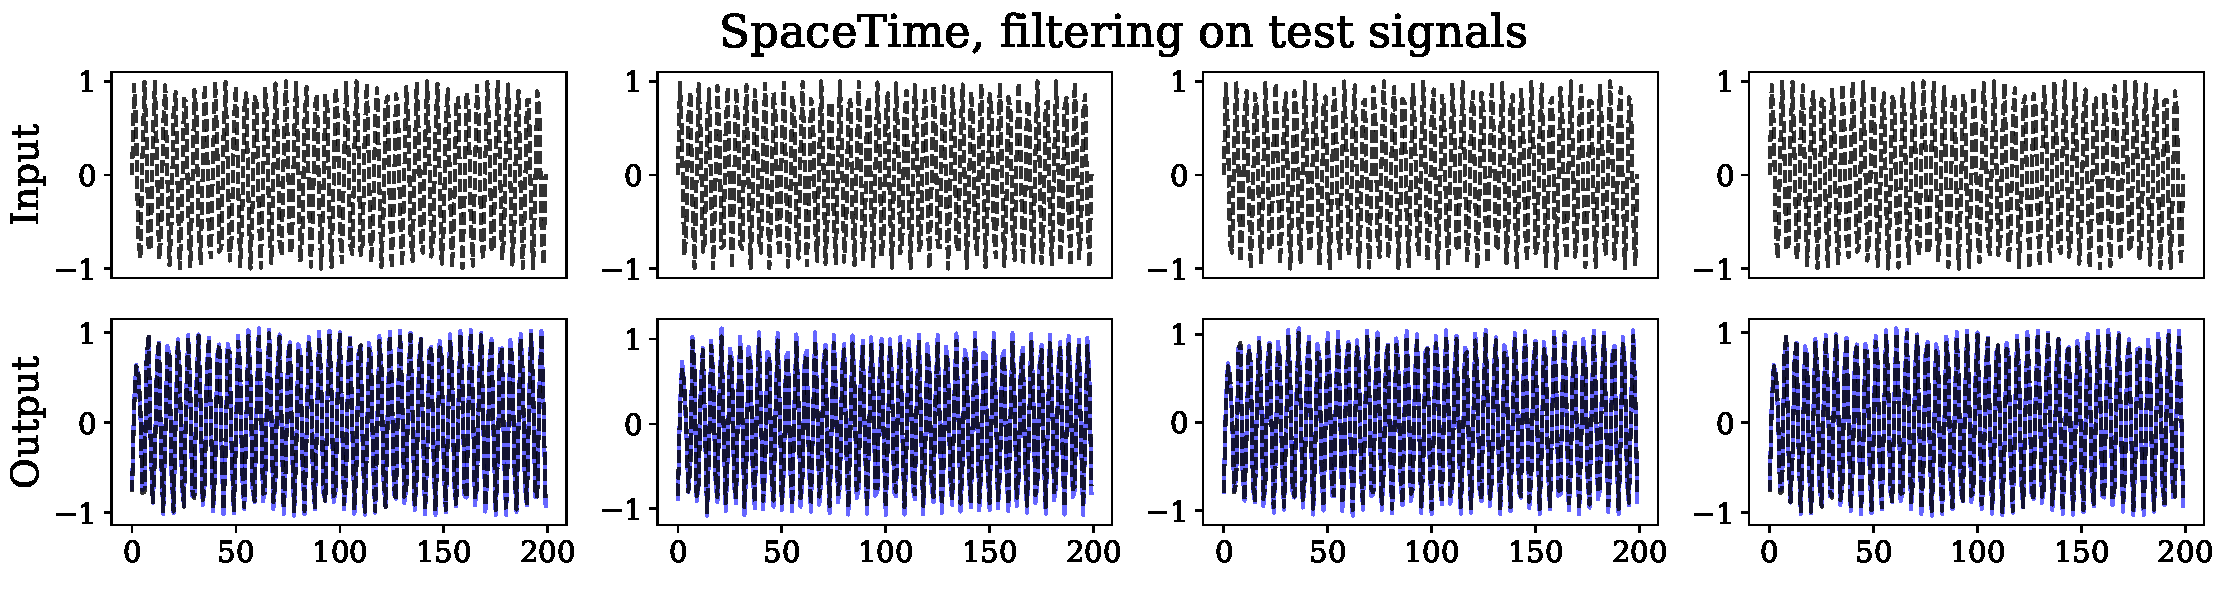
\includegraphics[width=0.99\columnwidth]{_ICLR2023_paper/figures/dsp_SpaceTime.pdf}
%     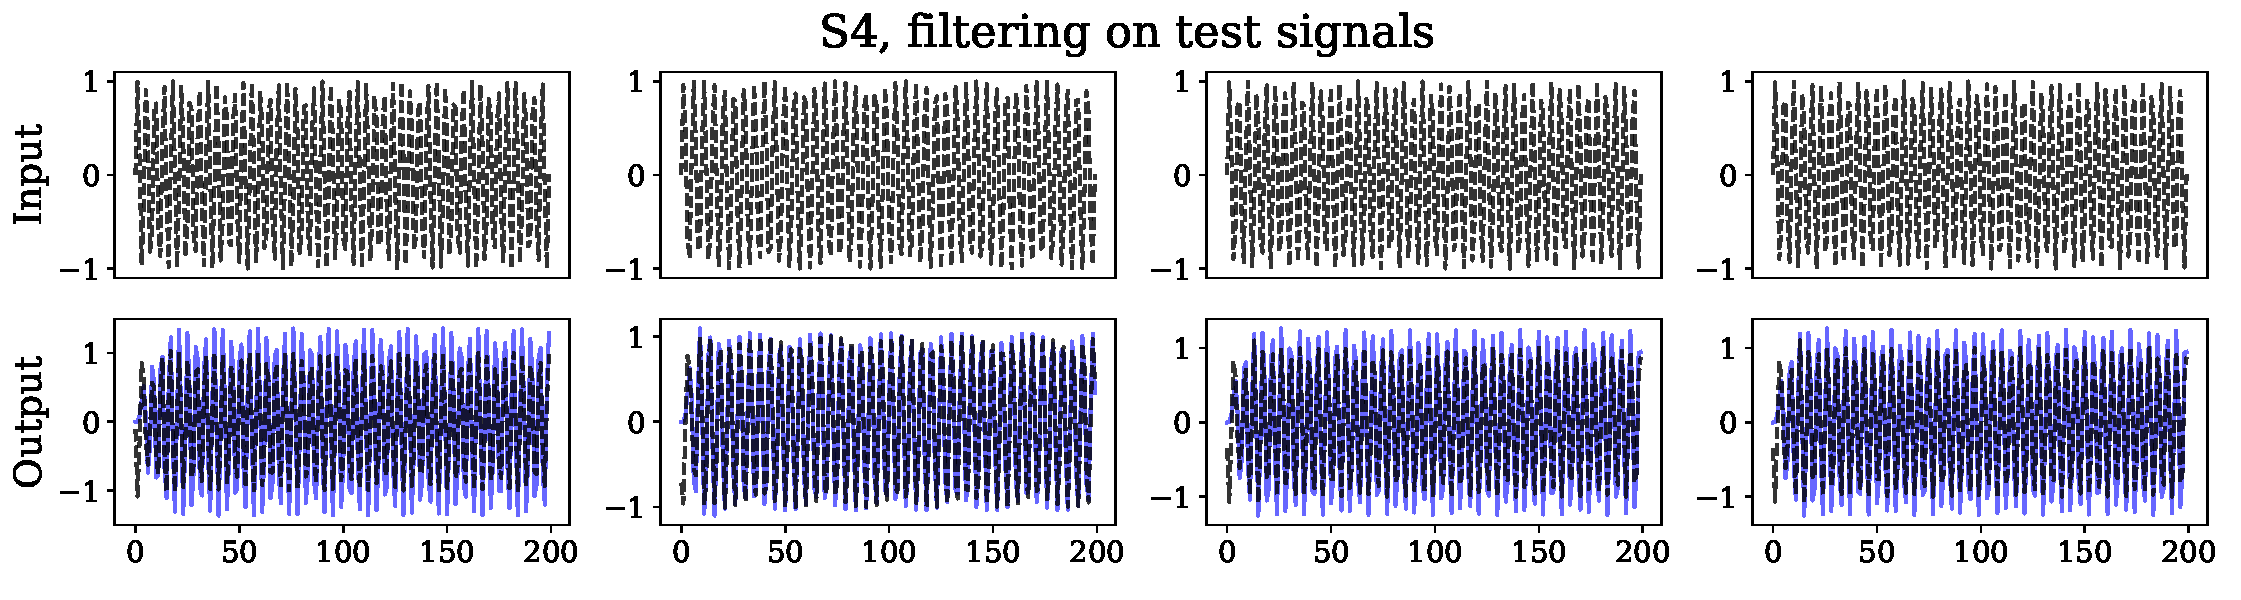
\includegraphics[width=0.99\columnwidth]{_ICLR2023_paper/figures/dsp_S4.pdf}
%     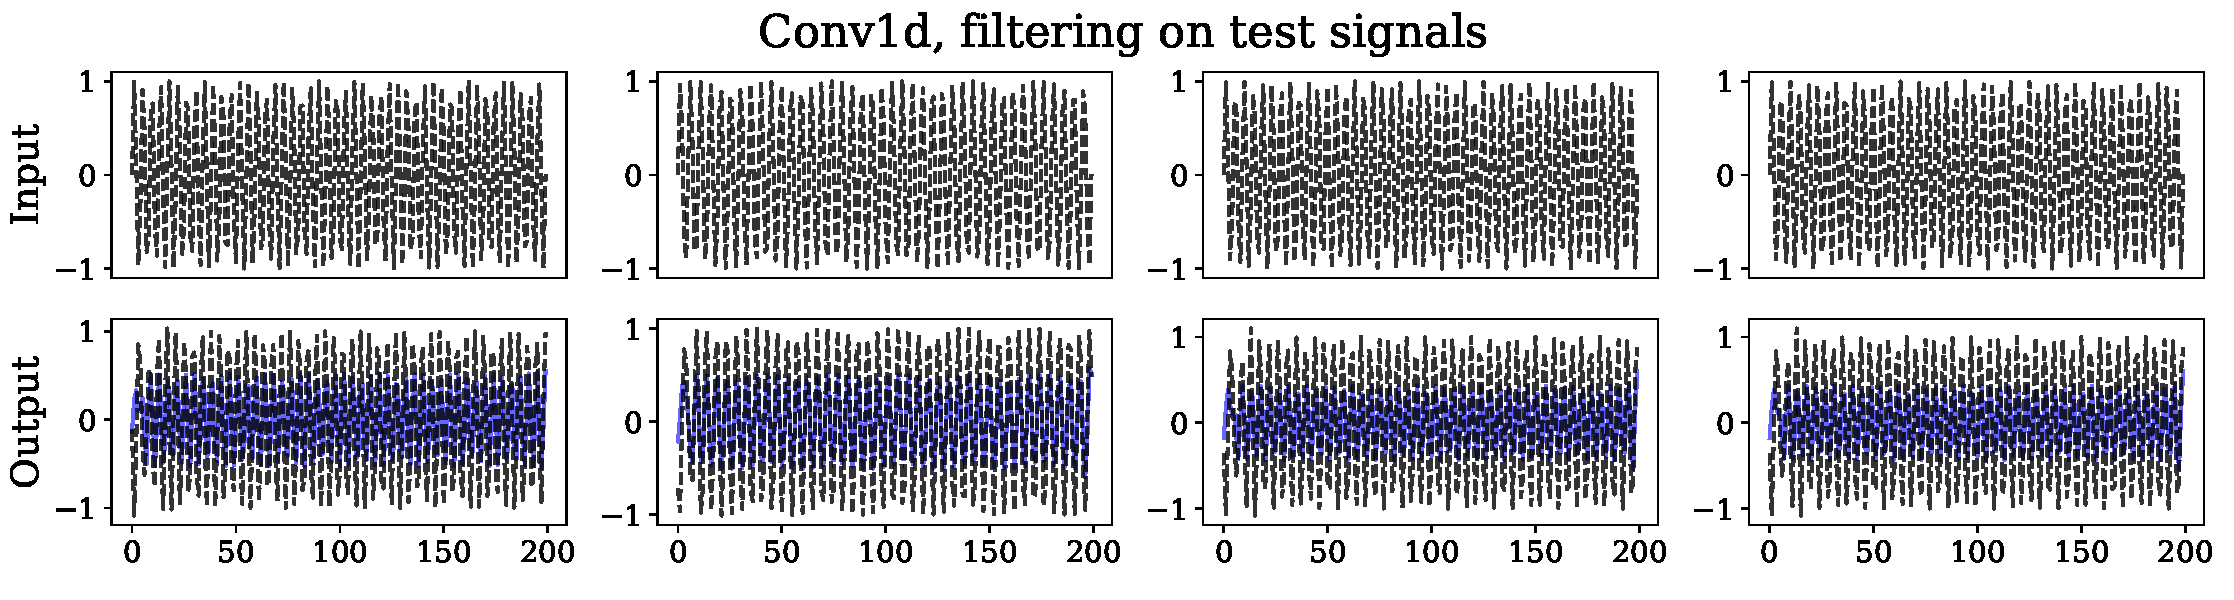
\includegraphics[width=0.99\columnwidth]{_ICLR2023_paper/figures/dsp_Conv1d.pdf}
%     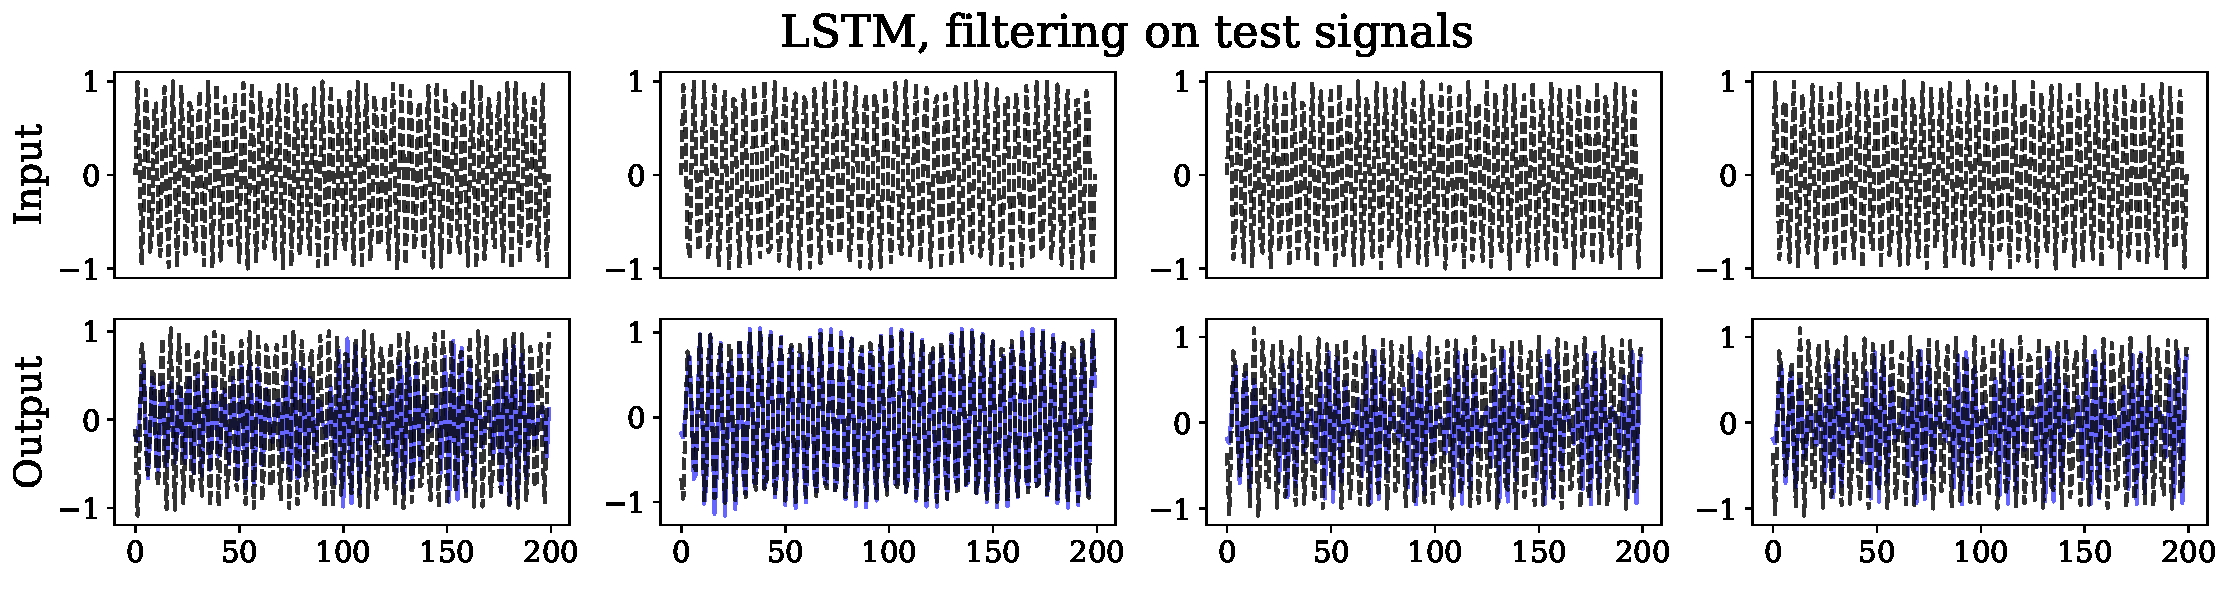
\includegraphics[width=0.99\columnwidth]{_ICLR2023_paper/figures/dsp_LSTM.pdf}
%     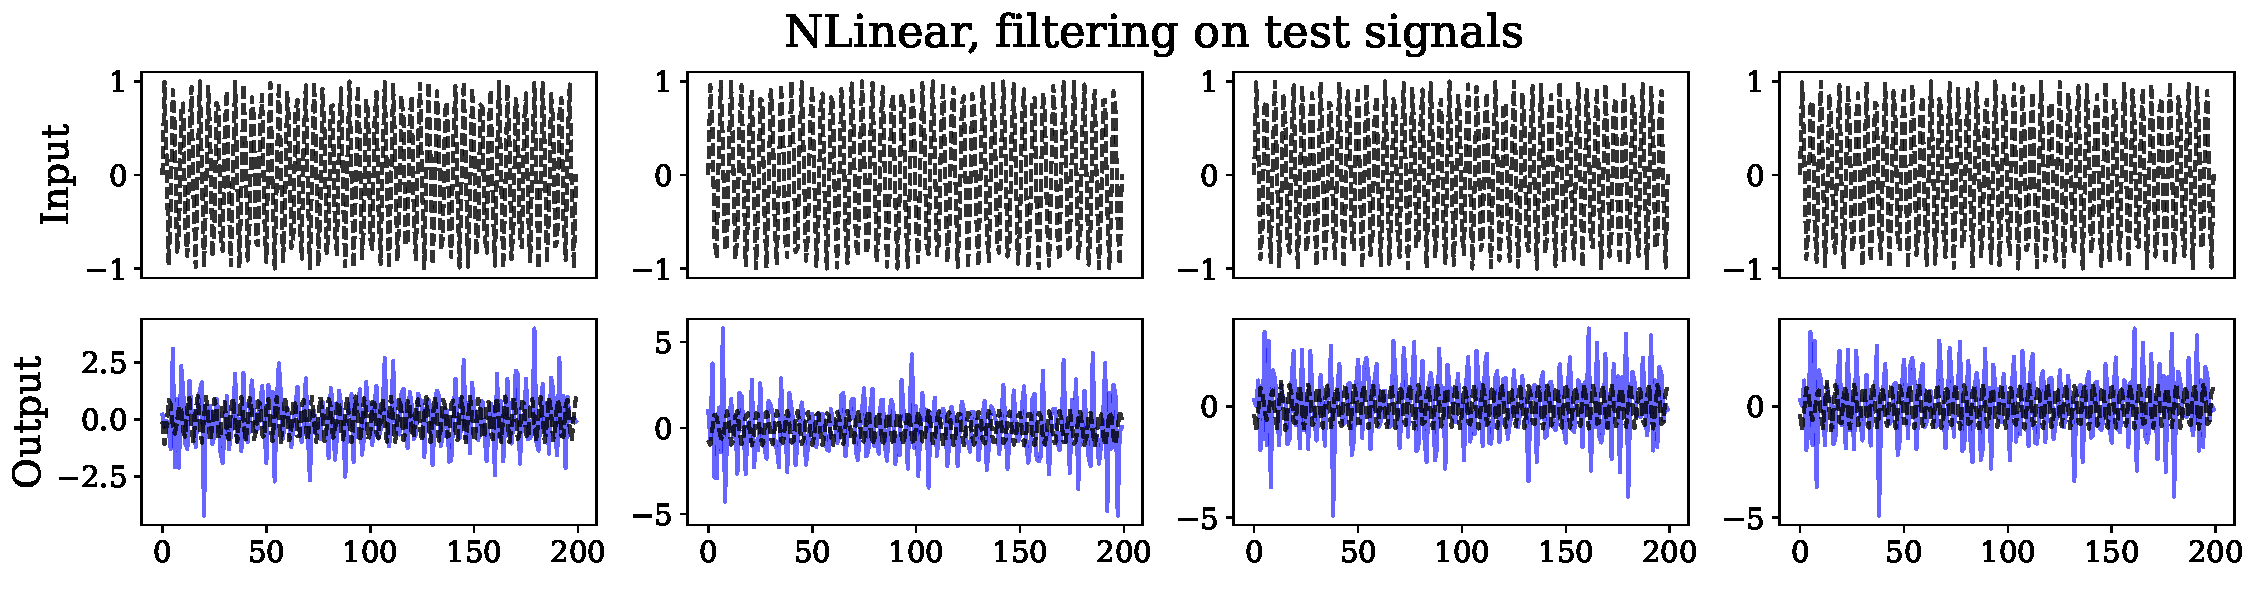
\includegraphics[width=0.99\columnwidth]{_ICLR2023_paper/figures/dsp_NLinear.pdf}
%     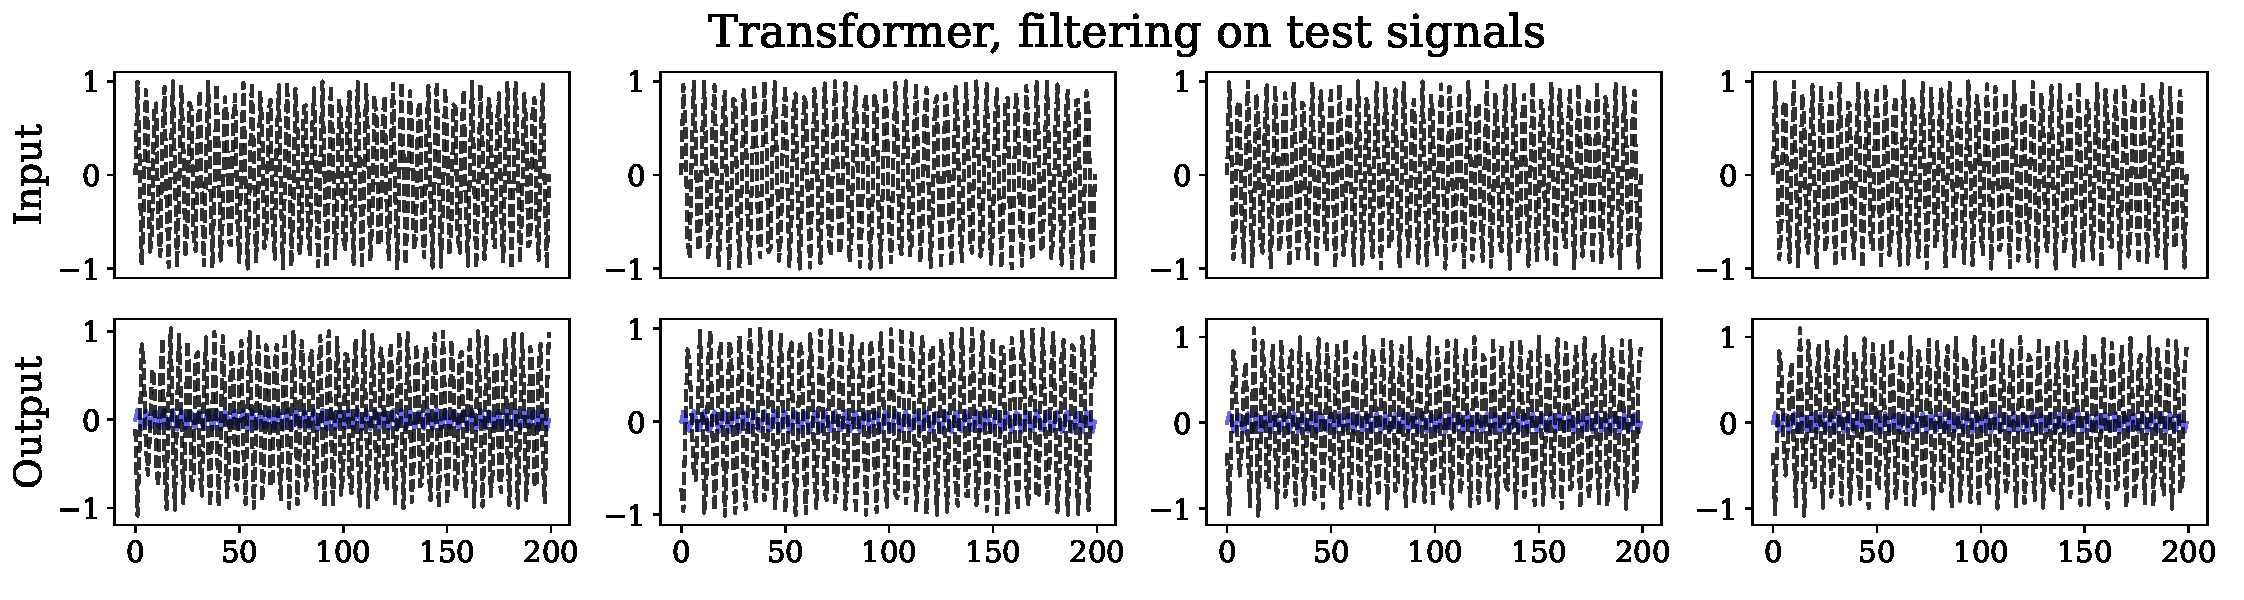
\includegraphics[width=0.99\columnwidth]{_ICLR2023_paper/figures/dsp_Transformer.pdf}
%     \vspace{-2mm}
%     \caption{Testing the capability of different sequence--to--sequence models to approximate the input--output map of digital filters. In blue, we show the output signal filtered by each model. The ground--truth digital filter is a Butterworth of order $10$.}
%     \label{fig:dsp_synthetic}
% \end{figure}
% %


% \begin{sidewaystable}[t]
%     \small
%     \centering
%     \begin{tabular}{c|c|cccccc|ccccc}
%     \toprule
%     %
%     Dataset  & \ourmethod & SES & Theta & TBATS & ETS & (DHR-)ARIMA & PR & CatBoost & DeepAR & N-BEATS & WaveNet & Transformer \\
%     %
%     \midrule
%     M1 Yearly & \underline{135508.3} & 193829.5 & 171458.1 & \textbf{116850.9} & 167739.0 & 175343.8 & 152038.7 & 237644.5 & 173075.1 & 192489.8 & 312821.8 & 182850.6 \\
    
%     M1 Quarterly & \underline{2200.3} & 2545.7&	2282.7	&2673.9&	2408.5&	2538.5&	1909.3&	2161.0& 2313.3&	2267.3&	2271.7&	2231.5  \\    
    
%     M1 Monthly & 2601.1 & 2725.8 & 2564.9 & 2594.5 & 2264.0 & 2450.6 & 2478.8 & 2461.7 & 2202.2 & \textbf{2183.4} & 2578.9 & 3129.8  \\

%     M3 Yearly & 1412.4 & 1172.9&	1106.1&	1386.3	&1189.2	&1662.2	&1181.8&	1341.7&		1157.9&	1117.4&	1147.6&	1084.8 \\
    
%     M3 Quarterly & 676.1 & 670.6&	567.7&	653.6&	598.7&	650.8&	605.5&	698.0&	606.6&	582.8&	606.8&	819.2\\ 
    
%     M3 Monthly & 897.12 & 893.9	&754.0&	765.2	&755.3&	790.8&	830.0&	874.2&	873.7&	796.9&	845.3&	948.4 \\
    
%     M3 Other & 265.56 & 309.7	&242.1&	217.0&	224.1	&220.8	&262.3&	349.9&	277.7&	248.5&	277.0	&271.0 \\
    
%     M4 Quarterly & 718.2 & 732.8&	673.2&	672.7&	674.3&	710.0&	711.9&	714.2&	700.3&	684.7&	697.0&	739.1 \\
    
%     M4 Monthly & 1092.2 & 755.5	&683.7&	743.4&	705.7&	702.1&	720.5&	734.8&	740.3&	705.2&	787.9&	902.4\\ 
    
%     M4 Weekly & \textbf{348.3}& 412.6	&405.2&	356.7&	408.5	&386.3&	350.3&	420.8&	422.2&	330.8&	437.3&	456.9\\ 
    
%     M4 Daily &\textbf{183.2}& 209.8&	210.4&	\underline{208.4}&	230.0	&212.6&	213.0&	263.1	&343.5&	221.7&	220.5&	233.6\\ 
    
%     M4 Hourly & \textbf{255.2} & 1476.8	&1483.7	&469.9&	3830.4&	1563.1&	\underline{313.0} &	344.6&	1095.1&	501.2&	468.1&	391.2\\
    
%     Tourism Yearly & \textbf{74799.2}& 106665.2&	99914.2&	105799.4&	104700.5&	106082.6&	89645.6	&87489.0&	78470.7&	78241.7	&77581.3&	80089.3\\
    
%     Tourism Quarterly & 11608.32& 15000.0&	9254.6&	12001.5	&10812.3	&12564.8	&11746.9	&12788.0	&11762.0&	11306.0	&11546.6	&11724.1 \\
    
%     Tourism Monthly & 3181.2& 7039.4&	2702.0	&3661.5	&2543.0	&3132.4&	2739.4&	3102.8&	2359.9&	2596.2&	2694.2&	2660.1\\
    
%     Pedestrian & 69.6& 228.1&	228.2	&261.3&	278.3&	820.3&	61.8&	60.8&	65.8&	99.3&	68.0&	70.2\\
    
%     Weather & \textbf{2.7}& 2.9	&3.3&	2.9&	3.0&	3.1	&9.1&	3.1&	\textbf{2.7}	&3.1&	3.0	&2.8\\
    
%     NN5 Weekly & \textbf{16.9}& 18.8&	18.7&	18.5&	18.8&	18.6&	18.6&	18.7&	18.5&	17.4&	24.2&	24.0 \\
    
%     Solar $10$ min &7.4& 7.2&	7.2	&10.7&	7.2	&5.6&	7.2	&8.7&	7.2	&6.6&	8.0&	7.2\\
    
%     Solar Weekly &1423.7& 1331.3&	1341.6&	1049.0&	1264.4&	967.9&	1168.2&	1754.2&	873.6&	1307.8&	2569.3&	693.8\\
    
%     Electricity Hourly & \textbf{475.1} & 1026.3&	1026.4&	743.4&	1524.9&	1082.4&	689.9&	582.7&	\underline{478.0} &	510.9&	489.9&	514.7\\
    
%     Electricity Weekly &37802.2& 77067.9&	76935.6&	28039.7	&70369.0&	32594.8&	47802.1&	37289.7	&53100.3&	35576.8	&63916.9&	78894.7\\
    
%     Fred-MD &3743.6& 3103.0&	3898.7&	2295.7&	2341.7	&3312.5&	9736.9&	2679.4&	4638.7&	2813.0&	2779.5&	5098.9\\
    
%     Traffic Hourly &0.03& 0.04&	0.04	&0.05&	0.04	&0.04&	0.03	&0.03&	0.02&	0.02	&0.03&	0.02\\
    
%     Traffic Weekly &\textbf{1.3}& 1.5&	1.5	&1.5&	1.5	&1.5&	1.5&	1.5	&1.5&	1.4	&1.6&	1.9\\
    
%     Hospital &40.1& 26.6&	22.6&	21.3&	22.0	&23.7&	23.5&	23.5&	22.0&	24.2&	23.4&	40.5\\
    
%     Covid &490.1& 403.4&	370.1&	113.0&	102.1&	100.5&	394.1&	607.9&	230.5&	186.5&	1135.4&	480.0\\
    
%     Saugeen & \textbf{24.0} & 39.8	&39.8	&42.6&	50.4&	43.2&	47.7&	\underline{39.3} &	45.3&	48.9&	43.0&	49.1\\
    
%     US Births &630.2& 1369.5&	735.5&	606.5&	607.2&	705.5&	732.1&	618.4&	684.0&	627.7&	768.8&	686.5\\
    
%     Sunspot &3.1& 5.0	&5.0&	3.0	&5.0&	3.0	&4.0&	2.4	&1.1&	14.5&	0.7	&0.5\\
    
%     Car Parts & 0.64 & 0.71&	0.65	&0.71&	0.71&	0.71&	\underline{0.58}&	0.71&	\textbf{0.50}&	1.0&	\underline{0.58}&	0.5\\
    
%     Vehicle Trips &30.4& 36.5&	37.4&	25.7&	37.6&	35.0&	31.7&	27.3&	26.5&	33.6&	29.0&	33.0\\
%     \bottomrule
%     %
%     \end{tabular}
%     \caption{Monash forecasting. We report test RMSE of \ourmethod for each dataset (best result selected via validation RMSE, average of $3$ runs).}
%     \label{tab:monash}
% \end{sidewaystable}


% \begin{table}[t]
%     \small
%     \centering
%     \begin{tabular}{c|cccc}
%     \toprule
%     %
%     Dataset  & Ours & S4S & S4D & S4DPLR  \\
%     %
%     \midrule
%     M1 Yearly & {\color{red!50}$154770.78$} & {\color{red!50}$177978.63$} & $161463.53$ &  \\
%     M1 Quarterly \\
%     M1 Monthly \\
%     M3 Yearly \\
%     M3 Quarterly \\ 
%     M3 Other \\ 
%     M4 Monthly \\ 
%     M4 Weekly \\ 
%     M4 Daily \\ 
%     Tourism Yearly \\
%     Tourism Monthly \\
%     Dominick \\
%     Pedestrian \\
%     Weather
%     NN5 \\
%     Solar $10$ min & $6.72$ &\\
%     Solar Weekly \\
%     Electricity Hourly \\
%     Electricity Weekly \\
%     Fred-MD \\
%     Traffic Hourly \\
%     Traffic Weekly \\
%     Hospital \\
%     Covid \\
%     Saugeen \\
%     US Births \\
%     \bottomrule
%     %
%     \end{tabular}
%     \caption{Monash forecasting. We report average test RMSE of \ourmethod for each dataset ($5$ runs each).}
%     \label{tab:my_label}
% \end{table}


% \begin{sidewaystable}[t]
%     \small
%     \centering
%     \begin{tabular}{c|c|cccccc|ccccc}
%     \toprule
%     %
%     Dataset  & Ours & SES & Theta & TBATS & ETS & (DHR-)ARIMA & PR & CatBoost & FFNN & DeepAR & N-BEATS & WaveNet & Transformer \\
%     %
%     \midrule
%     M1 Yearly & $2$ & $11$ & $6$ & $1$ & $5$ & $8$ & $3$ & $12$ & $4$ & $7$ & $10$ & $13$ & $9$ \\
%     M1 Quarterly \\
%     M1 Monthly \\
%     M3 Yearly \\
%     M3 Quarterly \\ 
%     M3 Other \\ 
%     M4 Monthly \\ 
%     M4 Weekly \\ 
%     M4 Daily \\ 
%     Tourism Yearly \\
%     Tourism Monthly \\
%     Dominick \\
%     Pedestrian \\
%     Weather
%     NN5 \\
%     Solar $10$ min & $6.72$ &\\
%     Solar Weekly \\
%     Electricity Hourly \\
%     Electricity Weekly \\
%     Fred-MD \\
%     Traffic Hourly \\
%     Traffic Weekly \\
%     Hospital \\
%     Covid \\
%     Saugeen \\
%     US Births \\
%     \bottomrule
%     %
%     \end{tabular}
%     \caption{Monash foreacasting. Model rankings (based on test RMSE).}
%     \label{tab:my_label}
% \end{sidewaystable}
\section{Experiment Details}
\label{sec:experiment_details}

\subsection{Model Configurations and Hyperparameters}

We summarize the details required to replicate our experiments below.

\subsubsection{Image Classification}

\textbf{Baseline Model:} For dense models, we use standard implementations of
ViT~\citep{dosovitskiy2020image}, MLP-Mixer{tolstikhin2021mlp} from the
\texttt{timm} library and from the T2T-ViT codebase~\citep{yuan2021tokens}.

The Monarch version of these models simply swap out the dense weight matrices in the attention blocks (projection matrices) and in the FFN block (linear layers) with Monarch matrices.
We set the number of blocks in the block-diagonal matrices to 4.
We also reduce the amount of regularization (stochastic depth) as our Monarch models are smaller than the dense models.

We adopt the hyperparameters (optimizer, learning rate, learning rate
scheduler) from~\citet{yuan2021tokens}.
Details are in~\cref{table:imagenet_hparams}.

We measure the wall-clock training time on V100 GPUs.

\begin{table}[!htbp]
 \caption{Configuration of the ImageNet experiment}   
\centering
\resizebox{0.8\linewidth}{!}{
\noindent\begin{tabular}{@{}c||ccccccc@{}}
  \specialrule{.15em}{.05em}{.05em}
Model&\multicolumn{1}{c}{Optimizer}&\multicolumn{1}{c}{Weight Decay}&\multicolumn{1}{c}{Learning Rate}&\multicolumn{1}{c}{Drop Path}&\multicolumn{1}{c}{Warmup/Epoch}\\
  \specialrule{.15em}{.05em}{.05em}
ViT-Small& AdamW & 0.05 & 0.001 & 0.1& 5/300 \\
Monarch-ViT-Small& AdamW & 0.05 & 0.001 &0& 5/300 \\
ViT-Base& AdamW & 0.05 & 0.001 &0.1& 5/300 \\
Monarch-ViT-Base& AdamW & 0.05 & 0.001 &0& 5/300 \\
  \specialrule{.15em}{.05em}{.05em}
Mixer-Small &AdamW& 0.1 &0.001&0.1& 5/300 \\
Monarch-Mixer-Small &AdamW&0.1 &0.001& 0 & 5/300 \\
Mixer-Base &AdamW& 0.1 &0.001&0.1& 5/300 \\
Monarch-Mixer-Base &AdamW &0.1 &0.001& 0 & 5/300 \\
  \specialrule{.15em}{.05em}{.05em}
\end{tabular}
}
\label{table:imagenet_hparams}
\end{table}

We follow the naming convention in the Vision Transformer paper and MLP-Mixer paper. In particular, ViT-S and ViT-B refers to the small and base ViT models respectively, and 16 refers to the patch size of 16x16. The MLP-Mixer models follow the same convention.

\subsubsection{Language Modeling}
For dense models, we use standard implementations of
GPT-2~\citep{radford2019language} from Huggingface \texttt{transformers} library and from Nvidia's Megatron-LM repo. 
We follow the training recipe of the Megatron-LM repo.

The Monarch version of these models simply swap out the dense weight matrices in the attention blocks (projection matrices) and in the FFN block (linear layers) with Monarch matrices.
We set the number of blocks in the block-diagonal matrices to 4.
We also reduce the regularization strength (dropout) as our model is smaller.

We report the hyperparameters used in~\cref{table:wt103} and~\cref{table:owt}.
We use an effective batch size of 512, and use gradient accumulation to fit into available GPU memory.

We measure the wall-clock training time on V100 GPUs.
\begin{table}[!h]
    \vspace{-0.5cm}
\centering
\caption{Configuration of the WikiText-103 experiments}
\resizebox{0.8\linewidth}{!}{
\noindent\begin{tabular}{@{}c||ccccccc@{}}
  \specialrule{.15em}{.05em}{.05em}
Model&\multicolumn{1}{c}{Optimizer}&\multicolumn{1}{c}{Weight Decay}&\multicolumn{1}{c}{Learning Rate}&\multicolumn{1}{c}{Dropout}&\multicolumn{1}{c}{Warmup/Epoch}\\
  \specialrule{.15em}{.05em}{.05em}
GPT-2-small& AdamW & 0.1 & 6e-4 & 0.1& 10/100 \\
Monarch-GPT-2-small& AdamW & 0.1 & 6e-4 & 0.0 & 10/100 \\
GPT-2-medium& AdamW & 0.1 & 1.5e-4 & 0.1& 10/100 \\
Monarch-GPT-2-medium & AdamW & 0.1 & 1.5e-4 & 0.0 & 10/100 \\
  \specialrule{.15em}{.05em}{.05em}
\end{tabular}
}
\label{table:wt103}
\end{table}

\begin{table}[!h]
\vspace{-0.5cm}
\centering
\caption{Configuration of the OpenWebText experiments}
\resizebox{0.8\linewidth}{!}{
\noindent\begin{tabular}{@{}c||ccccccc@{}}
  \specialrule{.15em}{.05em}{.05em}
Model&\multicolumn{1}{c}{Optimizer}&\multicolumn{1}{c}{Weight Decay}&\multicolumn{1}{c}{Learning Rate}&\multicolumn{1}{c}{Dropout}&\multicolumn{1}{c}{Warmup/Total iterations}\\
  \specialrule{.15em}{.05em}{.05em}
GPT-2-Small& AdamW & 0.1 & 6e-4 & 0.1& 4k/400k \\
Monarch-GPT-2-Small & AdamW & 0.1 & 6e-4 & 0.0 & 4k/400k \\
GPT-2-Medium& AdamW & 0.1 & 1.5e-4 & 0.1& 4k/400k \\
Monarch-GPT-2-Medium & AdamW & 0.1 & 1.5e-4 & 0.0 & 4k/400k \\
  \specialrule{.15em}{.05em}{.05em}
\end{tabular}
}
\label{table:owt}
\end{table}


\subsection{Details for PDE Solving}
We adopt the experiment setting and data generation of Navier-Stokes Equation from FNO~\citep{li2020fourier}. It considers the 2-d Navier-Stokes equation for a viscous, incompressible fliud in vorticity form on the unit tortus:
\begin{align}
    \partial_{t} w(x, t) + u(x, t) \cdot \nabla w(x, t) & = v \Delta w(x, t) + f(x), & x \in (0, 1)^2, t \in (0, T] \\
    \nabla w(x, t) & = 0, & x \in (0, 1)^2, t \in (0, T] \\
    w(x, 0) & = w_0(x), & x \in (0, 1)^2 \\
\end{align}
where $u \in C([, T0])$;$H_{per}((0, 1)^2; \mathbb{R}^2))$ for any $r>0$ is the velocity field, $w=\nabla \times u$ is the vorticity, $w_0 \in L^2_{per}((0, 1)^2; \mathbb{R})$ is the initial vorticity, $v \in \mathbb{R_{+}}$ is the viscosity coefficient, and $f \in L_{per}^2((0, 1)^2; \mathbb{R})$ is the forcing function. 
$T$ represents the time interval since it is time-dependent equation. $v$ represents the viscosity. N represents the number of training pairs or data. \cref{table:pde} shows the results for viscosities $v=1e-3, 1e-4, 1e-5$, $T=50, 30, 20$ respectively and use $N=1000$. 

\subsection{Details for GPT-2 Downstream Tasks}
We train Pixelfly-GPT2-small on a larger scale dataset, OpenWebText, and evaluate the downstream quality on zero-shot generation and classification tasks from~\citep{zhao2021calibrate}, achieving comparable and even better performance to the dense model. Specifically, the datasets contains five popular classification tasks: SST2, Trec, CB, Agnews, and Dbpedia. We also adapated the calibrated metric from~\citep{zhao2021calibrate} for evaluation. Results for each individual task are shown in~\cref{table:gpt_finetune_full}. 

\begin{table}[h]
  \small
  \centering
  \vspace{-3mm}
  \caption{\label{table:gpt_finetune_full}The performance (accuracy) of GPT-2-medium trained with Monarch reverse sparsification and with conventional dense training on text classification benchmarks.}
  \setlength{\tabcolsep}{5pt}
  \vspace{1em}
   \resizebox{0.7\linewidth}{!}{
  \begin{tabular}{@{}c||ccccc@{}}
    \specialrule{.15em}{.05em}{.05em}
    Model&\multicolumn{1}{c}{OpenWebText (ppl)}&\multicolumn{1}{c}{Speedup}& \multicolumn{1}{c}{Classification (avg acc)} \\
    \specialrule{.15em}{.05em}{.05em}
    GPT-2m& 68.3 & 37.0 & 10.7 & 52.0 & 26.6\\
    Monarch-GPT-2m& 72 & 38.6 & 12.5 & 47.3 & 23.0 \\
    \specialrule{.15em}{.05em}{.05em}
  \end{tabular}
  }
  \vspace{-3mm}
\end{table}

\subsection{Details for BERT Pretraining}
\label{subsec:bert_details}

We follow the training procedure and hyperparameters of the reference
implementation from Nvidia Deep Learning examples
(\url{https://github.com/NVIDIA/DeepLearningExamples}).
In particular, we use the LAMB optimizer with learning rate 4e-3.
We use as large a minibatch size as possible that still fits in the GPU memory
(A100-40GB), and use gradient accumulation to reach an effective batch size of
64k sequences for phase 1 (maximum sequence length 128) and 32k for phase 2
(maximum sequence legnth 512).
We train is mixed precision (fp16 and fp32).

We use all the optimizations that were in Nvidia's BERT implementation
in MLPerf 1.1:
\begin{enumerate}
  \item Only compute the prediction scores (last layer) for masked tokens as
  the outputs of other tokens are not used to compute the masked language
  modeling loss.
  \item Remove padding tokens and only compute the attention for non-padding
  tokens.
  \item Use a fused CUDA kernel (FMHA) that combines 4 steps into one kernel: computes
  $Q K^T$, take softmax, apply dropout, multiply by $V$, where $Q, K, V$ are the
  query, key, and value respectively.
  \item Fuse matrix multiplication and adding bias into one CUDA kernel in the feed-forward network
  (FFN) layers. The gradient of the bias is also fused with the matrix
  multiplication the backward pass.
  \item Fuse matrix multiplication and adding bias into one CUDA kernel in the
  attention output projection.
  \item Fuse dropout and adding residual in the residual connection at the end
  on the attention and FFN blocks.
\end{enumerate}

We train with DeepSpeed~\citep{rasley2020deepspeed} ZeRO optimizer stage 1 to
shard the optimizer states, thus reducing GPU memory usage and allowing us to
use larger batch sizes.
For the Nvidia MLPerf implementation, we report the speed for both Apex's
automatic mix-precision (AMP) level O2 (as in the original implementation), and
DeepSpeed ZeRO optimizer.

\subsection{Accelerated Multi-coil MRI Reconstruction}
\label{sec:experiment_details_mri}

\subsubsection{Background}
In multi-coil MRI, multiple receiver coils (i.e. sensors) acquire complex-valued measurements in the spatial frequency (a.k.a. \textit{k-space}) domain. These measurements are modulated by the spatially-varying sensitivity maps, which characterize the sensitivity of each coil to the imaging target. In accelerated MRI, scan times are reduced by decreasing the number of samples acquired in k-space. Because the data is sampled below the Nyquist rate, reconstructing the underlying image is an ill-posed problem.

The forward problem for accelerated multi-coil MRI can be written as the matrix equation
\begin{equation*}
    y = \Omega\boldsymbol{F}\boldsymbol{S}x + \epsilon
\end{equation*}
where $\Omega$ is the binary undersampling mask that indexes acquired samples in k-space, $y$ is the vectorized measured signal in k-space, $\boldsymbol{F}$ is the discrete Fourier transform matrix, $\boldsymbol{S}$ is the receiver coil sensitivity maps,  $x$ is the ground-truth signal in image-space, and $\epsilon$ is additive complex Gaussian noise. The acceleration factor is given by $R = \frac{\sum_i^{|N|} \Omega_i}{|\Omega|}$.

\subsubsection{Experimental Details}

\paragraph{Dataset.} We benchmark our method on the SKM-TEA Raw Data Track, which consists of dual-echo 3D MRI scans \citep{desai2021skm}. Scans are accelerated using Poisson Disc undersampling masks distributed with the dataset. During training, Poisson Disc masks are generated, cached, and applied to mask the k-space data to simulate accelerated scans.

\paragraph{Matrix Shape.} Like all matrices, Monarch matrices have an explicit shape constraint, which is a limitation of these matrices for MRI reconstruction tasks. Thus, the SKM-TEA dataset was filtered to include scans of shape $512 \times 512 \times 160$, which is the most frequently occuring scan shape. A total of 3 scans were dropped from the original 155 scans in the dataset. Our method and all baselines were trained on this filtered dataset.

\begin{table}[!ht]
    \vspace{-0.5cm}
\centering
\caption{Baseline configurations of the SKM-TEA MRI reconstruction experiments.}
\resizebox{0.6\linewidth}{!}{
\noindent\begin{tabular}{c||cccccc}
  \specialrule{.15em}{.05em}{.05em}
Model & Params & Optimizer & Weight Decay & Learning Rate & Epoch \\
  \specialrule{.15em}{.05em}{.05em}
SENSE & --- & --- & --- & --- & --- \\
U-Net &  7.8M & Adam & 1e-4 & 1e-3 & 20 \\
mSENSE  & 57.5K & Adam & 1e-4 & 1e-3 & 20 \\
  \specialrule{.15em}{.05em}{.05em}
\end{tabular}
}
\label{table:skmtea-config}
\end{table}


\paragraph{Baselines.} We compare our method to two baselines, SENSE and U-Net. Parameter count and hyperparameters are available in Table \ref{table:skmtea-config}.
\begin{itemize}
    \item \textit{SENSE}: SENSE performs a linear combination of the images acquired on each coil \citep{pruessmann1999sense}. Here, the inverse fsat Fourier transform (IFFT) is applied to the acquired k-space for each coil. The resulting images are combined into a single complex image by weighting each coil image by corresponding coil sensitivity maps. In accelerated MRI, the unsampled frequencies are zero-valued; thus, SENSE produces a \textit{zero-filled image}. Note, SENSE does not require any training.
    \item \textit{U-Net}: U-Net is a popular fully convolutional neural network baseline for MRI reconstruction \citep{ronneberger2015u}. We use the default implementation and hyperparameters used by \citet{desai2021skm} to benchmark the SKM-TEA dataset. In this approach, the SENSE-reconstructed zero-filled image is mapped to SENSE-reconstructed ground truth images.
\end{itemize}

\paragraph{Monarch-SENSE (mSENSE):} We propose a modification to the SENSE method, in which the (IFFT) is parameterized by a factorized Monarch matrix. This matrix is initialized to the IFFT but, unlike SENSE, is learnable. While mSENSE is trainable, it has 137x fewer trainable parameters than U-Net.

\paragraph{Metrics:} We evaluate reconstruction performance using peak signal-to-noise ratio (pSNR) and structural similarity (SSIM) on both echoes (echo1 - E1, echo2 - E2) separately. Both metrics were computed on the 3D volume of each echo.

\paragraph{Extended Results.} We provide sample reconstructions of SENSE, mSENSE, and U-Net in data-limited settings for first (Fig.~\ref{fig:mri-data-limited-echo1}) and second (Fig.~\ref{fig:mri-data-limited-echo2}) echoes. Both SENSE and U-Net reconstructed images have aliasing artifacts. Due to the random Poisson Disc undersampling pattern, these artifacts are incoherent, causing them to manifest as blurring around fine structures and edges. In contrast, mSENSE can recover these structures with higher fidelity. Even in the second echo, which has lower signal-to-noise ratio (SNR) than the first echo, mSENSE does not overblur the image.

\begin{figure}
    \centering
    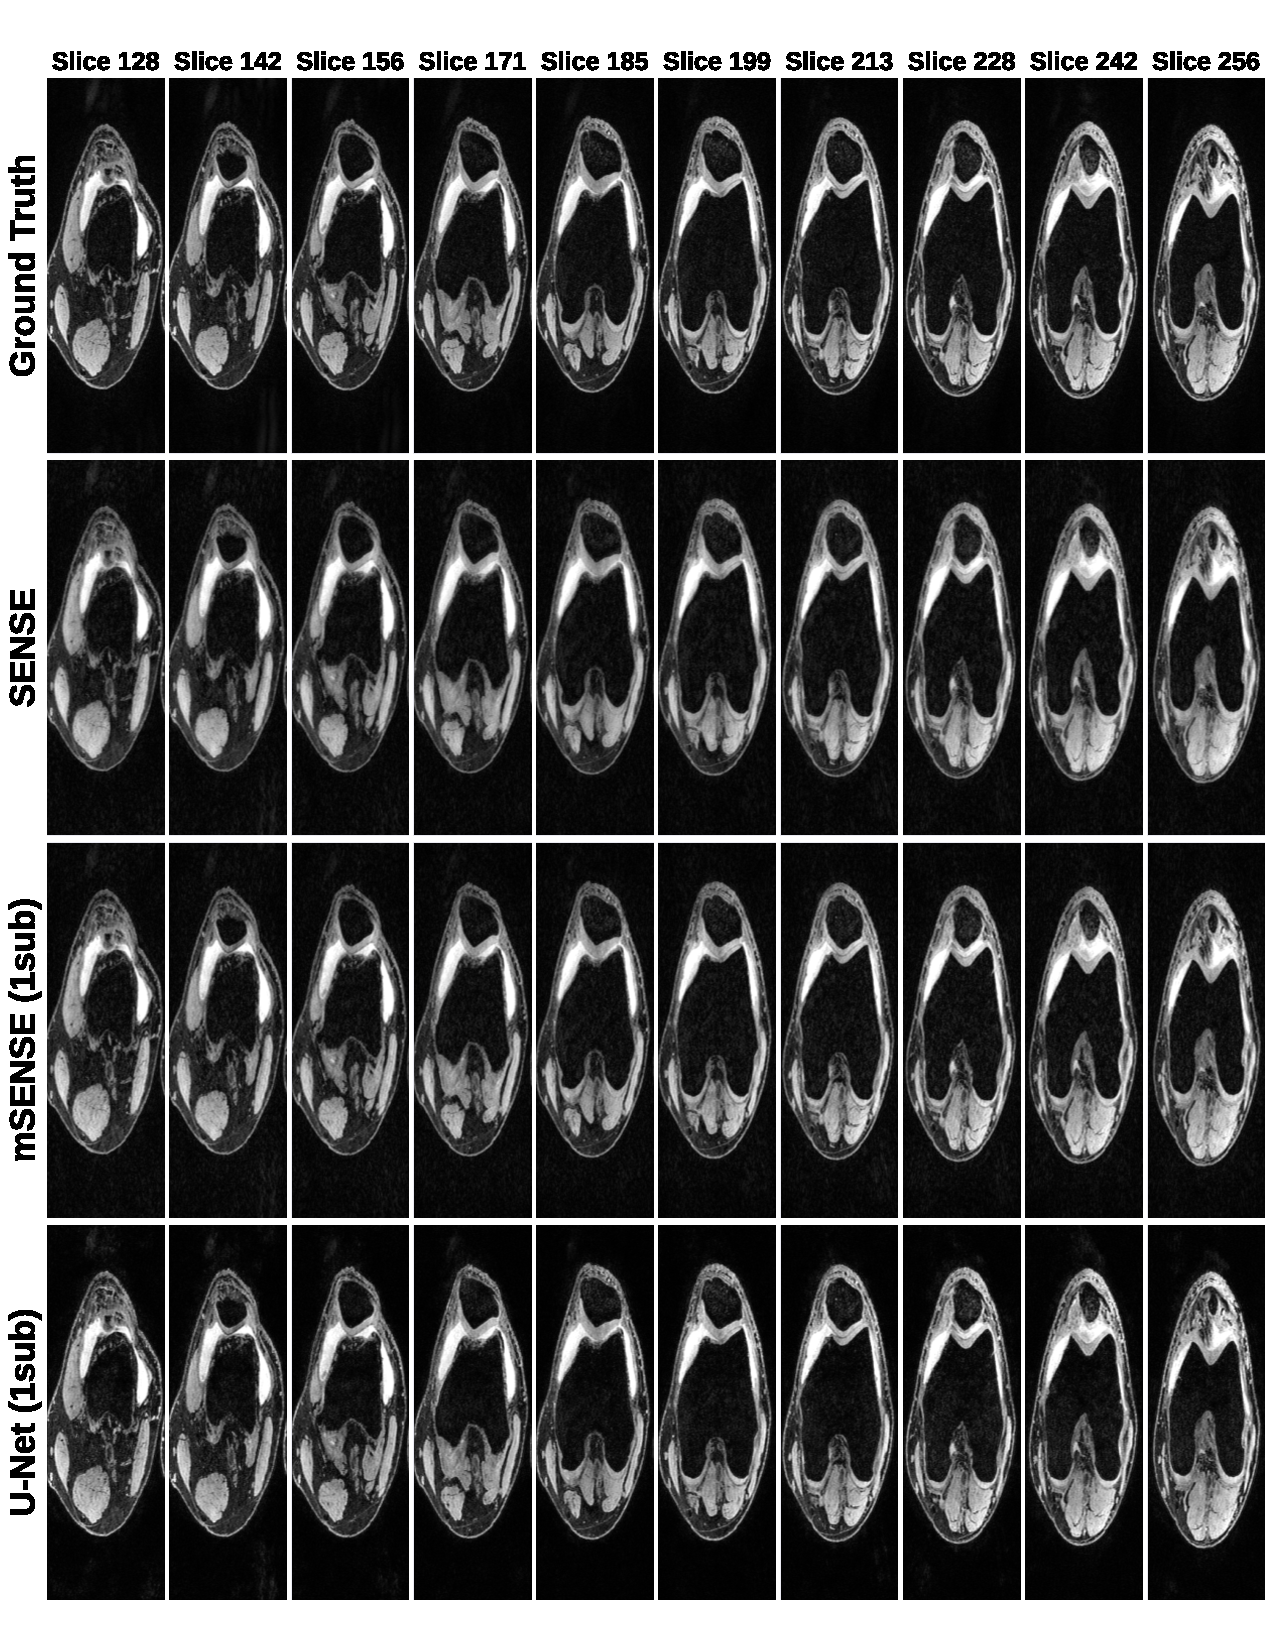
\includegraphics[width=0.9\linewidth]{figures/sample-mri-echo1.pdf}
    \vspace{-1em}
    \caption{Sample reconstructions at 2x acceleration for the first echo in the SKM-TEA dataset using SENSE, Monarch-SENSE (mSENSE), and U-Net. Both mSENSE and U-Net are trained with 1 training scan. SENSE is an untrained method.}
    \label{fig:mri-data-limited-echo1}
\end{figure}

\begin{figure}
    \centering
    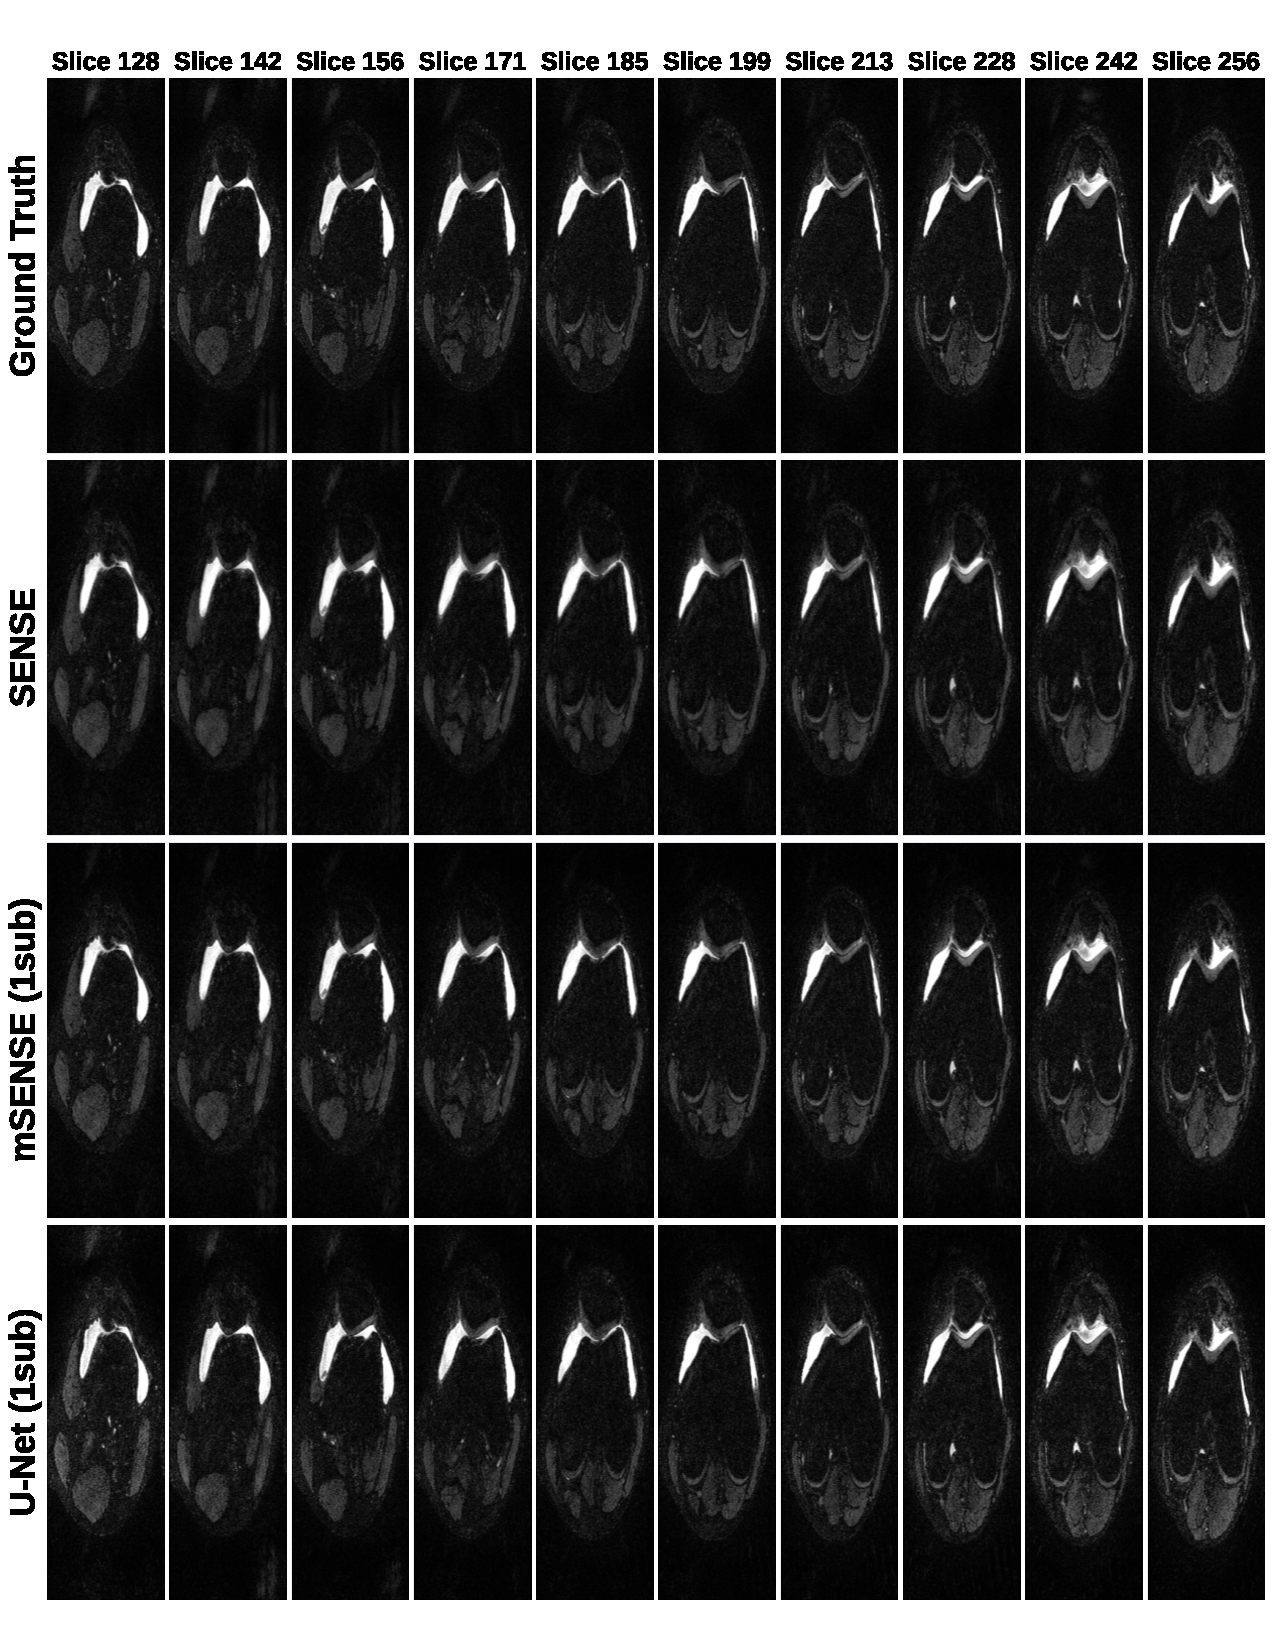
\includegraphics[width=6in]{figures/sample-mri-echo2.pdf}
    \vspace{-1em}
    \caption{Sample reconstructions at 2x acceleration for the second echo in the SKM-TEA dataset using SENSE, Monarch SENSE (mSENSE), and U-Net. Both mSENSE and U-Net are trained with 1 training scan. SENSE is an untrained method.}
    \label{fig:mri-data-limited-echo2}
\end{figure}







\section{Extended experimental results} \label{app:exp_results}

\subsection{Expressivity on digital filters}

% {\ourmethod{} can approximate the frequency response of digital filters}

We experimentally verify whether \ourmethod{} can approximate the input--output map of digital filter admitting a state--space representation, with improved generalization over baseline models given test inputs of unseen frequencies.

We generate a dataset of $1028$ sinusoidal signals of length $200$
\[
x(t) = \sin{(2\pi \omega t})
\]
where $\omega \in [2, 40]~\bigcup~[50, 100]$ in the training set and $\omega \in (40, 50)$ in the test set. The outputs are obtained by filtering $x$, i.e., $y = \mathcal{F}(x)$  where $\mathcal{F}$ is in the family of digital filters. 

We introduce common various sequence-to-sequence layers or models as baselines: the original S4 diagonal plus low--rank \citep{gu2021efficiently}, a single-layer LSTM, a single 1d convolution (Conv1d), a dense linear layer (NLinear), a single self--attention layer. All models are trained for $800$ epochs with batch size $256$, learning rate $10^{-3}$ and Adam. We repeat this experiment for digital filters of different orders \citep{oppenheim1999discrete}. The results are shown in Figure \ref{fig:dsp_synthetic}. \ourmethod{} learns to match the frequency response of the target filter, producing the correct output for inputs at test frequencies. 


\begin{table}[h]
\caption{Comparing sequence models on the task of approximating the input--output map defined by digital filters of different orders. Test RMSE on held-out inputs at unseen frequencies.}
    \label{tab:my_label}
    \centering
    \begin{tabular}{cc|ccccccc}
    \toprule
    %
    Filter & Order & \ourmethod & S4 & Conv1D & LSTM & NLinear & Transformer \\
    %
    \midrule
    Butterworth & $2$ & $0.0055$ & $0.0118$ & $0.0112$ & $0.0115$ & $1.8420$ & $0.5535$ \\
    & $3$ & $0.0057$ & $0.3499$ & $0.0449$ & $0.0231$ & $1.7085$ & $0.6639$ \\
    & $10$ & $0.0039$ & $0.8077$ & $0.4747$ & $0.2753$  & $1.5162$ & $0.7191$ \\
    \midrule
    Chebyshev $1$ & $2$ & $0.0187$ & $0.0480$ & $0.0558$ & $0.0285$ & $1.9313$ & $0.2452$ \\
    & $3$ & $0.0055$ & $0.0467$ & $0.0615$ & $0.0178$ & $1.8077$ & $0.4028$ \\
    & $10$ & $0.0620$ & $0.6670$ & $0.1961$ & $0.1463$ & $1.5069$ & $0.7925$ \\
    \midrule
    Chebyshev $2$ & $2$ & $0.0112$ & $0.0121$ & $0.0067$ & $0.0019$ & $0.4101$ & $0.0030$ \\
    & $3$ & $0.0201$ & $0.0110$ & $0.0771$ & $0.0102$ & $0.4261$ & $0.0088$\\
    & $10$ & $0.0063$ &  $0.6209$ & $0.3361$ & $0.1911$ & $1.5584$ & $0.7936$\\
    \midrule
    Elliptic & $2$ & $0.0001$ & $0.0300$ & $0.0565$ & $0.0236$ & $1.9150$ & $0.2445$ \\
    & $3$ & $0.0671$ & $0.0868$ & $0.0551$ & $0.0171$ & $1.8782$  & $0.4198$ \\
    & $10$ & $0.0622$ & $0.0909$ & $0.1352$ & $0.1344$ & $1.4901$ & $0.7368$ \\
    %
    \bottomrule
    %
    \end{tabular}
    
\end{table}
%
% \begin{figure}[h]
%     \centering
%     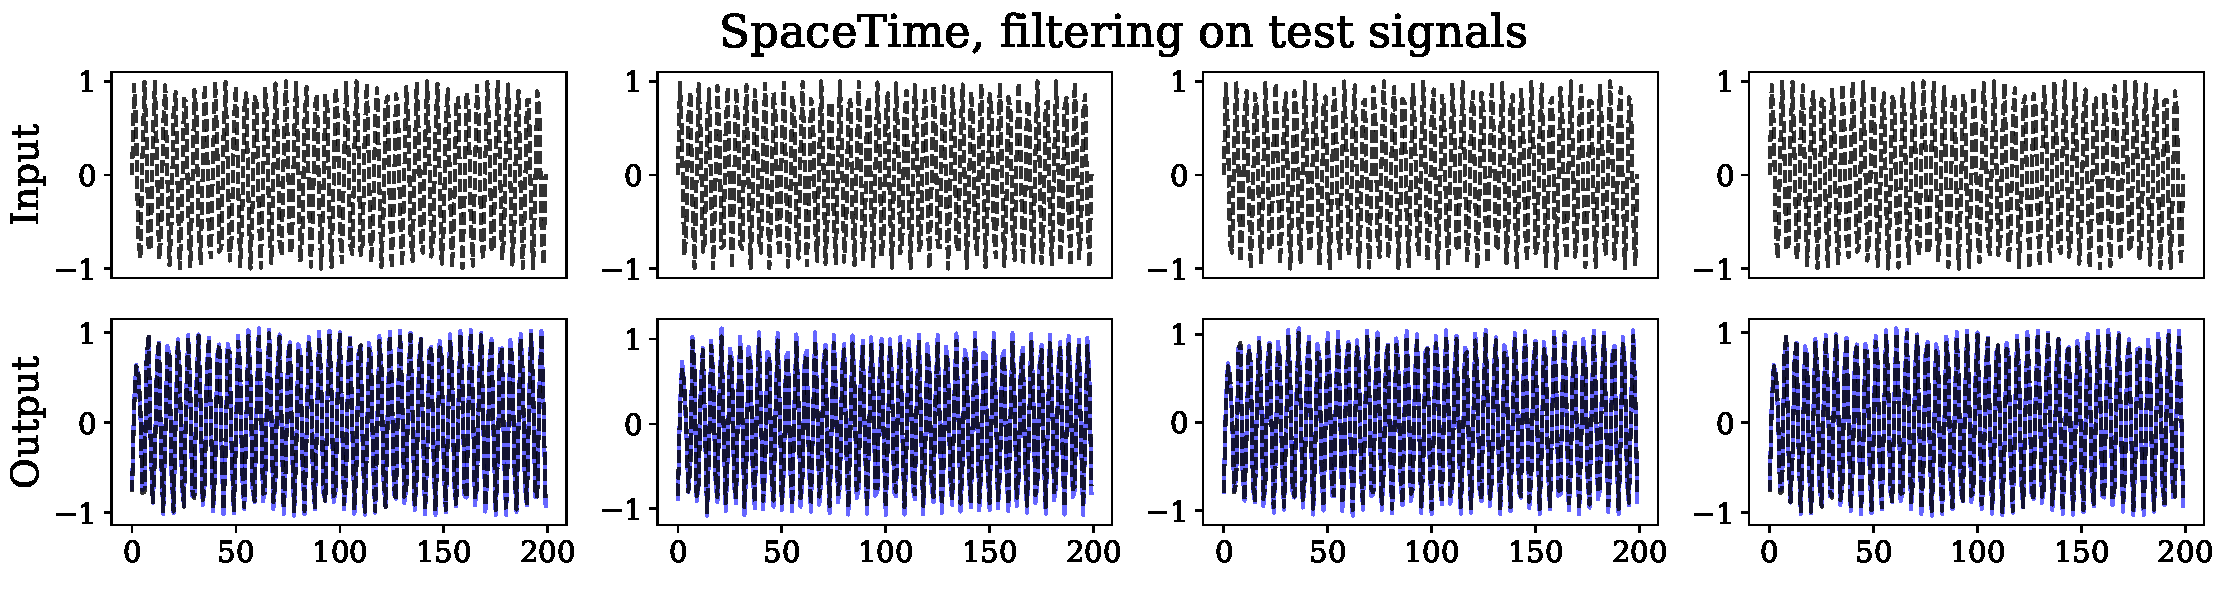
\includegraphics[width=0.99\columnwidth]{_ICLR2023_paper/figures/dsp_SpaceTime.pdf}
%     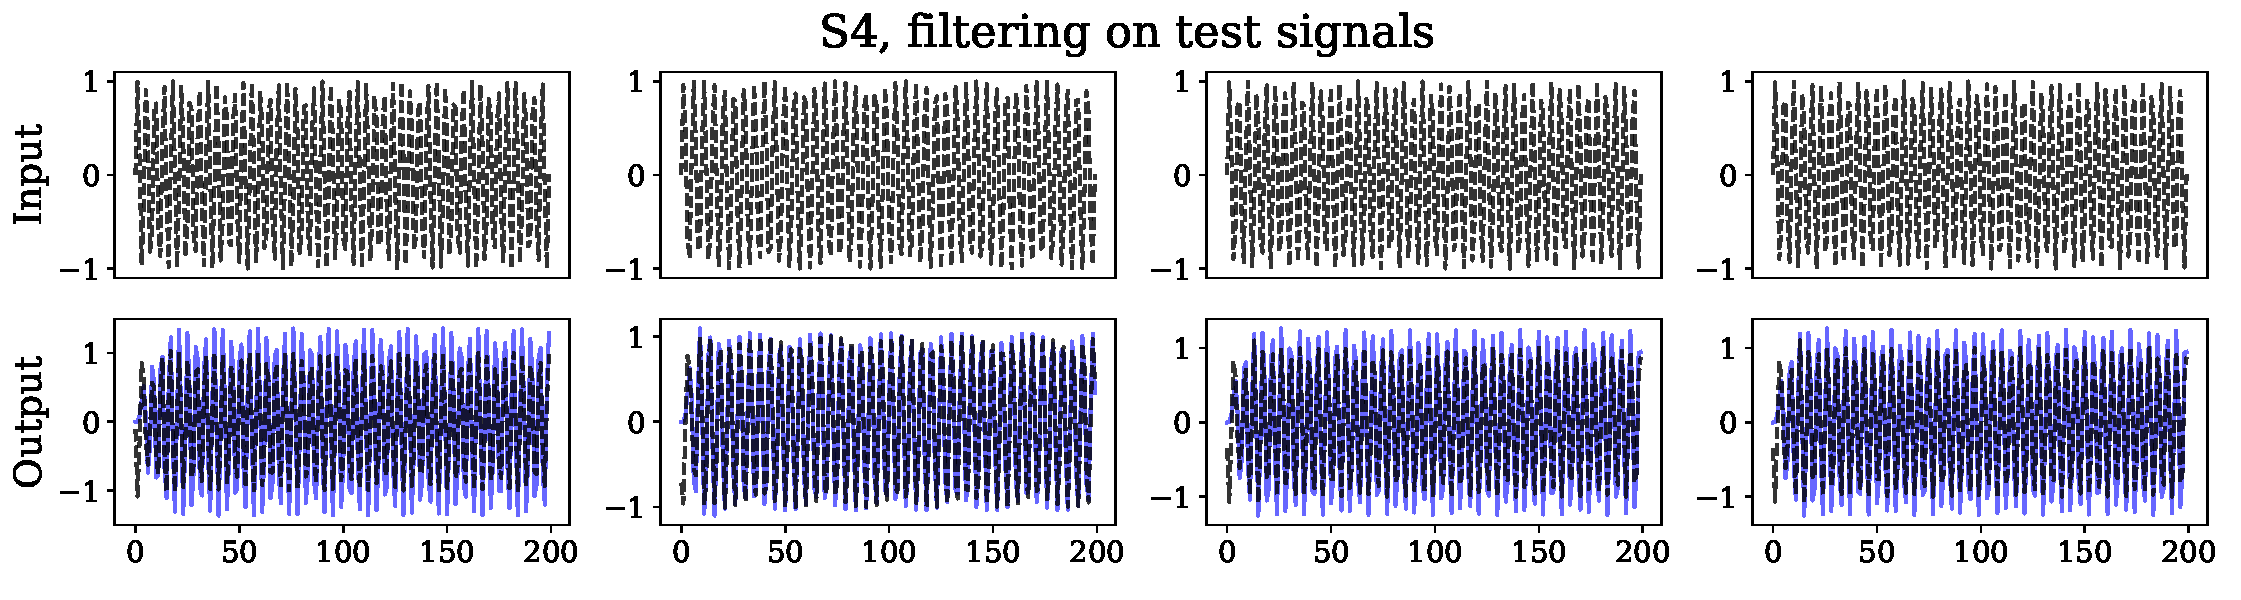
\includegraphics[width=0.99\columnwidth]{_ICLR2023_paper/figures/dsp_S4.pdf}
%     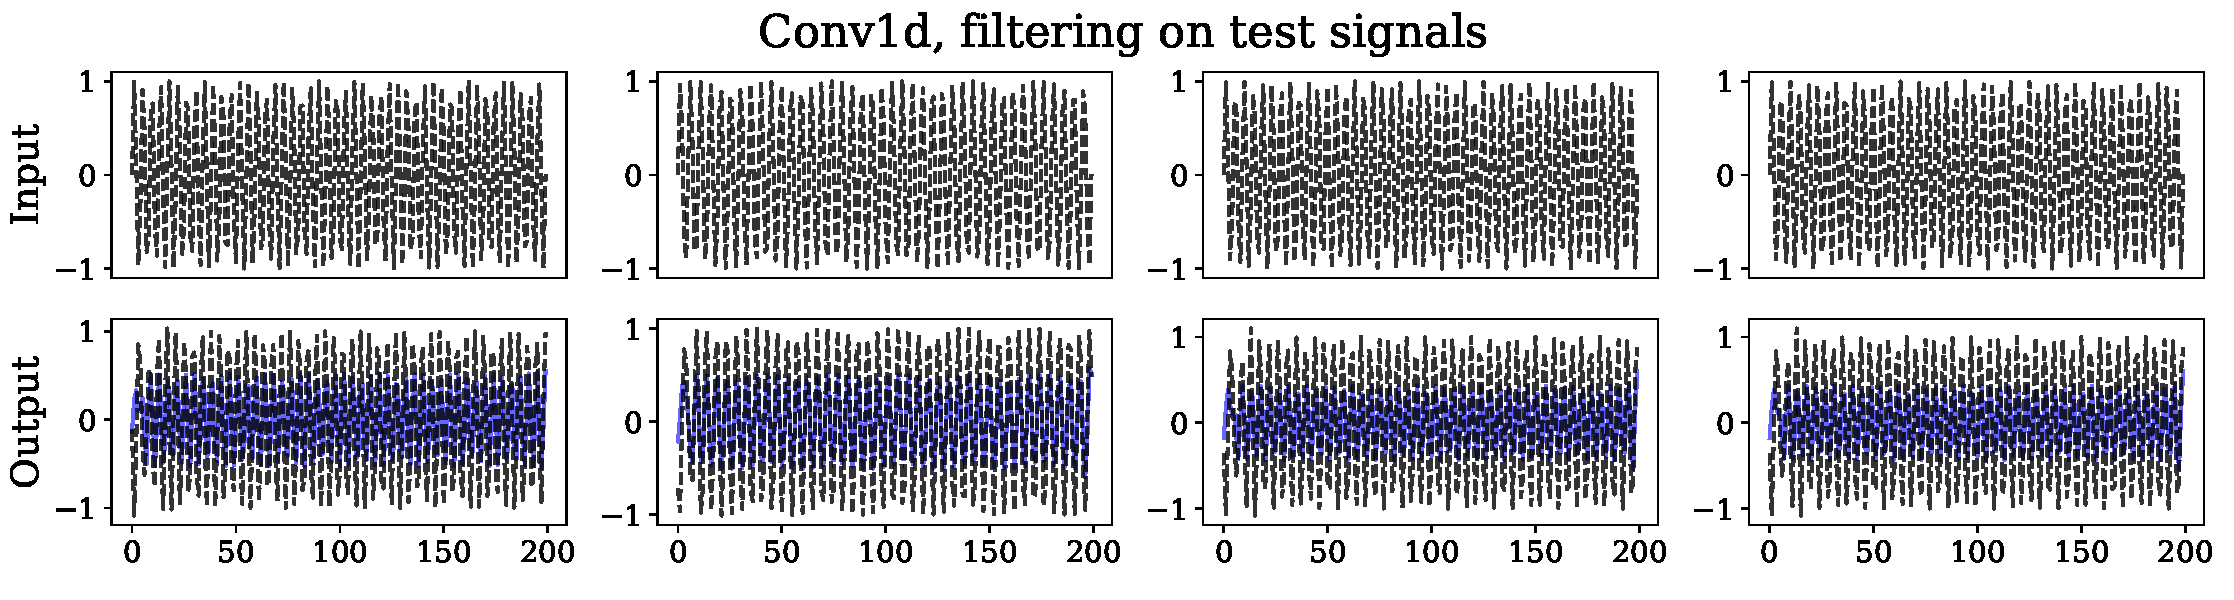
\includegraphics[width=0.99\columnwidth]{_ICLR2023_paper/figures/dsp_Conv1d.pdf}
%     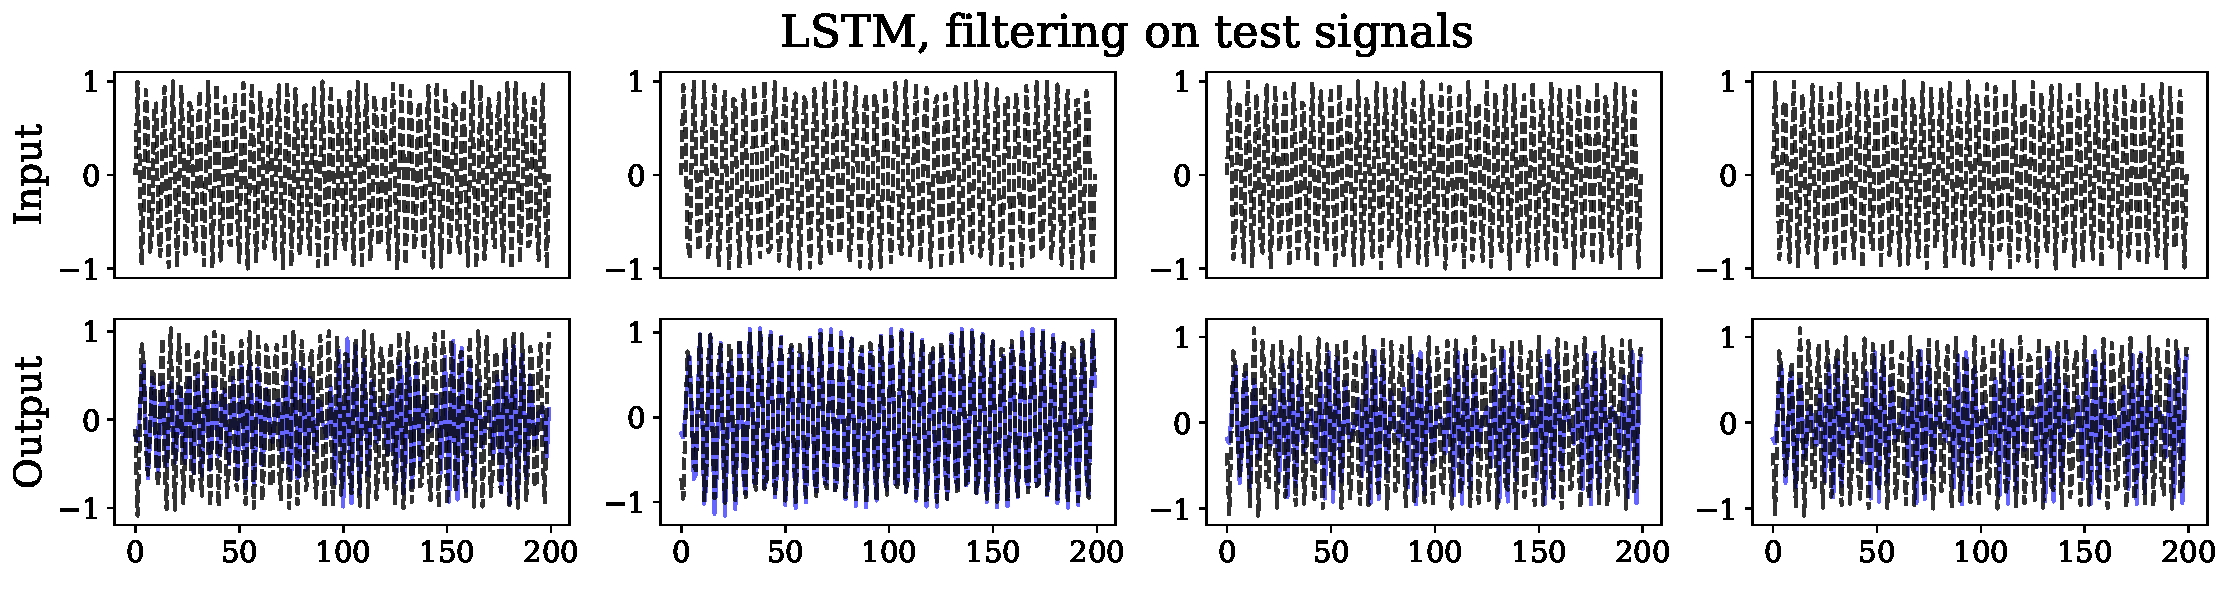
\includegraphics[width=0.99\columnwidth]{_ICLR2023_paper/figures/dsp_LSTM.pdf}
%     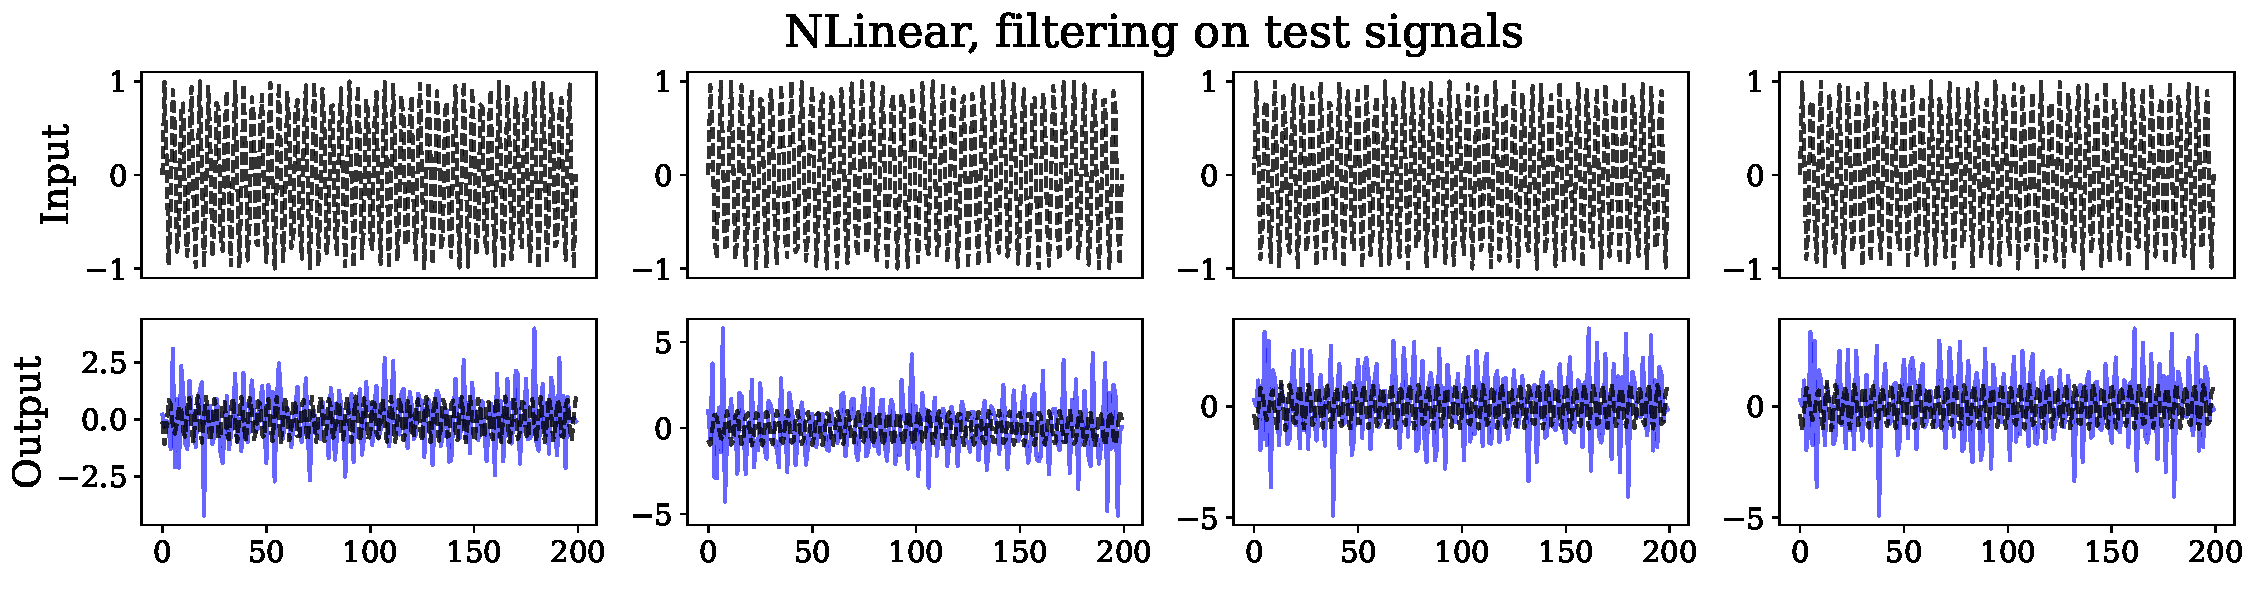
\includegraphics[width=0.99\columnwidth]{_ICLR2023_paper/figures/dsp_NLinear.pdf}
%     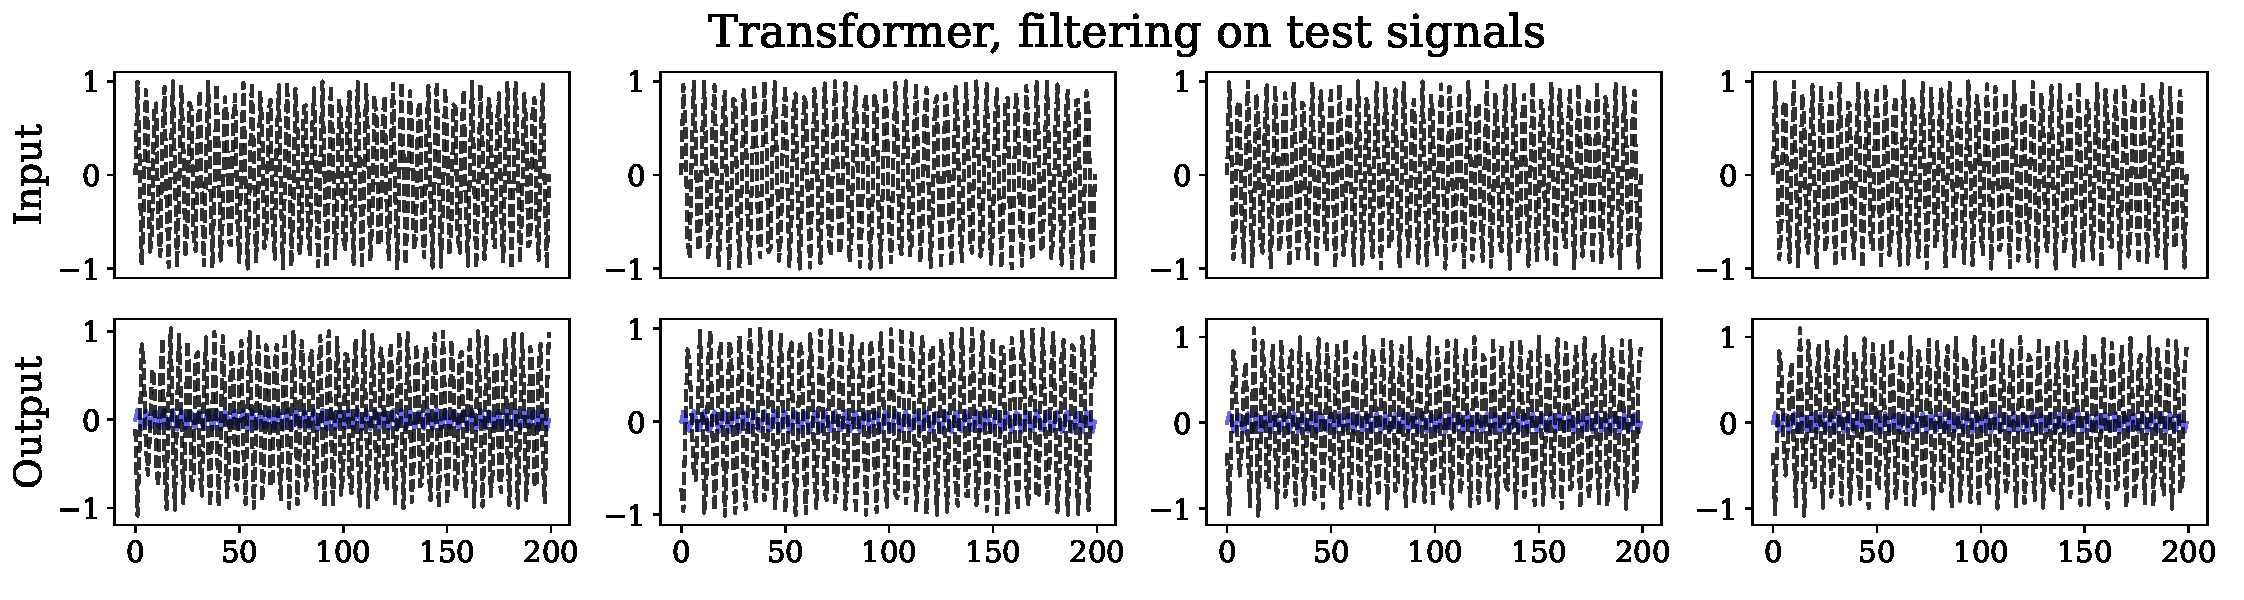
\includegraphics[width=0.99\columnwidth]{_ICLR2023_paper/figures/dsp_Transformer.pdf}
%     \caption{Testing the capability of different sequence--to--sequence models to approximate the input--output map of digital filters. In blue, we show the output signal filtered by each model. The ground--truth digital filter is a Butterworth of order $10$.}
%     \label{fig:dsp_synthetic}
% \end{figure}
% %




\subsection{Informer Forecasting}\label{appendix:informer_extended}

\textbf{Univariate long horizon forecasts with Informer splits.} Beyond the ETT datasets and horizons evaluated on in Table~\ref{tab:informer-s-long-original}, we also compare \ourmethod{} to alternative time series methods on the complete datasets and horizons used in the original Informer paper~\citep{zhou2021informer}. We compare against recent architectures which similarly evaluate on these settings, including ETSFormer~\citep{woo2022etsformer}, SCINet~\citep{liu2021time}, and Yformer~\citep{madhusudhanan2021yformer}, and other comparison methods found in the Informer paper, such as Reformer~\citep{kitaev2020reformer} and ARIMA.
\ourmethod{} obtains best results on 20 out of 25 settings, the most of any method.

\begin{table}[!t]
\caption{ \textbf{Univariate forecasting} results on Informer datasets. \textbf{Best} results in \textbf{bold}. \ourmethod{} obtains best MSE on 19 out of 25 and best MAE on 20 out of 25 dataset and horizon tasks.}
\resizebox{\linewidth}{!}{
\begin{tabular}{@{}c|cbcbcbcbcbcbcbcbcbcbcbcbc@{}}
% \begin{tabular}{@{}c|ccccccccccccccccccccccccc@{}}
\toprule
\multicolumn{2}{c}{Methods}        & \multicolumn{2}{c}{\textbf{\ourmethod{}}} & \multicolumn{2}{c}{ETSFormer}   & \multicolumn{2}{c}{SCINet} & \multicolumn{2}{c}{S4}          & \multicolumn{2}{c}{Yformer}     & \multicolumn{2}{c}{Informer} & \multicolumn{2}{c}{LogTrans} & \multicolumn{2}{c}{Reformer} & \multicolumn{2}{c}{N-BEATS} & \multicolumn{2}{c}{DeepAR} & \multicolumn{2}{c}{ARIMA} & \multicolumn{2}{c}{Prophet} \\ \midrule
\multicolumn{2}{c}{Metric}         & MSE                & MAE               & MSE            & MAE            & MSE          & MAE         & MSE            & MAE            & MSE            & MAE            & MSE           & MAE          & MSE           & MAE          & MSE           & MAE          & MSE          & MAE          & MSE          & MAE         & MSE         & MAE         & MSE          & MAE          \\ \midrule
\parbox[t]{2mm}{\multirow{5}{*}{\rotatebox[origin=c]{90}{ETTh1}}}   & 24  & \textbf{0.026}     & \textbf{0.124}    & 0.030          & 0.132          & 0.031        & 0.132       & 0.061          & 0.191          & 0.082          & 0.230          & 0.098         & 0.247        & 0.103         & 0.259        & 0.222         & 0.389        & 0.042        & 0.156        & 0.107        & 0.280       & 0.108       & 0.284       & 0.115        & 0.275        \\
\multicolumn{1}{c|}{}        & 48  & \textbf{0.038}     & \textbf{0.153}    & 0.041          & 0.154          & 0.051        & 0.173       & 0.079          & 0.220          & 0.139          & 0.308          & 0.158         & 0.319        & 0.167         & 0.328        & 0.284         & 0.445        & 0.065        & 0.200        & 0.162        & 0.327       & 0.175       & 0.424       & 0.168        & 0.330        \\
\multicolumn{1}{c|}{}        & 168 & 0.066              & 0.209             & \textbf{0.065} & \textbf{0.203} & 0.081        & 0.222       & 0.104          & 0.258          & 0.111          & 0.268          & 0.183         & 0.346        & 0.207         & 0.375        & 1.522         & 1.191        & 0.106        & 0.255        & 0.239        & 0.422       & 0.396       & 0.504       & 1.224        & 0.763        \\
\multicolumn{1}{c|}{}        & 336 & \textbf{0.069}     & \textbf{0.212}    & 0.071          & 0.215          & 0.094        & 0.242       & 0.080          & 0.229          & 0.195          & 0.365          & 0.222         & 0.387        & 0.230         & 0.398        & 1.860         & 1.124        & 0.127        & 0.284        & 0.445        & 0.552       & 0.468       & 0.593       & 1.549        & 1.820        \\
\multicolumn{1}{c|}{}        & 720 & \textbf{0.075}     & \textbf{0.226}    & 0.079          & 0.227          & 0.176        & 0.343       & 0.116          & 0.271          & 0.226          & 0.394          & 0.269         & 0.435        & 0.273         & 0.463        & 2.112         & 1.436        & 0.269        & 0.422        & 0.658        & 0.707       & 0.659       & 0.766       & 2.735        & 3.253        \\ \midrule
\parbox[t]{2mm}{\multirow{5}{*}{\rotatebox[origin=c]{90}{ETTh2}}}   & 24  & \textbf{0.064}     & \textbf{0.189}    & 0.087          & 0.232          & 0.070        & 0.194       & 0.095          & 0.234          & 0.082          & 0.221          & 0.093         & 0.240        & 0.102         & 0.255        & 0.263         & 0.437        & 0.078        & 0.210        & 0.098        & 0.263       & 3.554       & 0.445       & 0.199        & 0.381        \\
\multicolumn{1}{c|}{}        & 48  & \textbf{0.095}     & \textbf{0.230}    & 0.112          & 0.263          & 0.102        & 0.242       & 0.191          & 0.346          & 0.172          & 0.334          & 0.155         & 0.314        & 0.169         & 0.348        & 0.458         & 0.545        & 0.123        & 0.271        & 0.163        & 0.341       & 3.190       & 0.474       & 0.304        & 0.462        \\
\multicolumn{1}{c|}{}        & 168 & \textbf{0.144}     & \textbf{0.300}    & 0.169          & 0.325          & 0.157        & 0.311       & 0.167          & 0.333          & 0.174          & 0.337          & 0.232         & 0.389        & 0.246         & 0.422        & 1.029         & 0.879        & 0.244        & 0.393        & 0.255        & 0.414       & 2.800       & 0.595       & 2.145        & 1.068        \\
\multicolumn{1}{c|}{}        & 336 & \textbf{0.169}     & \textbf{0.333}    & 0.216          & 0.379          & 0.177        & 0.340       & 0.189          & 0.361          & 0.224          & 0.391          & 0.263         & 0.417        & 0.267         & 0.437        & 1.668         & 1.228        & 0.270        & 0.418        & 0.604        & 0.607       & 2.753       & 0.738       & 2.096        & 2.543        \\
\multicolumn{1}{c|}{}        & 720 & 0.188              & \textbf{0.352}    & 0.226          & 0.385          & 0.253        & 0.403       & \textbf{0.187} & 0.358          & 0.211          & 0.382          & 0.277         & 0.431        & 0.303         & 0.493        & 2.030         & 1.721        & 0.281        & 0.432        & 0.429        & 0.580       & 2.878       & 1.044       & 3.355        & 4.664        \\ \midrule
\parbox[t]{2mm}{\multirow{5}{*}{\rotatebox[origin=c]{90}{ETTm1}}}   & 24  & \textbf{0.010}     & \textbf{0.074}    & 0.013          & 0.084          & 0.019        & 0.088       & 0.024          & 0.117          & 0.024          & 0.118          & 0.030         & 0.137        & 0.065         & 0.202        & 0.095         & 0.228        & 0.031        & 0.117        & 0.091        & 0.243       & 0.090       & 0.206       & 0.120        & 0.290        \\
\multicolumn{1}{c|}{}        & 48  & \textbf{0.019}     & \textbf{0.101}    & 0.020          & 0.107          & 0.045        & 0.143       & 0.051          & 0.174          & 0.048          & 0.173          & 0.069         & 0.203        & 0.078         & 0.220        & 0.249         & 0.390        & 0.056        & 0.168        & 0.219        & 0.362       & 0.179       & 0.306       & 0.133        & 0.305        \\
\multicolumn{1}{c|}{}        & 96  & \textbf{0.026}     & \textbf{0.121}    & 0.030          & 0.132          & 0.072        & 0.198       & 0.086          & 0.229          & 0.143          & 0.311          & 0.194         & 0.372        & 0.199         & 0.386        & 0.920         & 0.767        & 0.095        & 0.234        & 0.364        & 0.496       & 0.272       & 0.399       & 0.194        & 0.396        \\
\multicolumn{1}{c|}{}        & 288 & \textbf{0.051}     & \textbf{0.176}    & 0.053          & 0.179          & 0.117        & 0.266       & 0.160          & 0.327          & 0.150          & 0.316          & 0.401         & 0.554        & 0.411         & 0.572        & 1.108         & 1.245        & 0.157        & 0.311        & 0.948        & 0.795       & 0.462       & 0.558       & 0.452        & 0.574        \\
\multicolumn{1}{c|}{}        & 672 & 0.078              & 0.220             & \textbf{0.075} & \textbf{0.214} & 0.180        & 0.328       & 0.292          & 0.466          & 0.305          & 0.476          & 0.512         & 0.644        & 0.598         & 0.702        & 1.793         & 1.528        & 0.207        & 0.370        & 2.437        & 1.352       & 0.639       & 0.697       & 2.747        & 1.174        \\ \midrule
\parbox[t]{2mm}{\multirow{5}{*}{\rotatebox[origin=c]{90}{Weather}}} & 24  & \textbf{0.088}     & \textbf{0.205}    & -              & -              & -            & -           & 0.125          & 0.254          & -              & -              & 0.117         & 0.251        & 0.136         & 0.279        & 0.231         & 0.401        & -            & -            & 0.128        & 0.274       & 0.219       & 0.355       & 0.302        & 0.433        \\
\multicolumn{1}{c|}{}        & 48  & \textbf{0.134}     & \textbf{0.258}    & -              & -              & -            & -           & 0.181          & 0.305          & -              & -              & 0.178         & 0.318        & 0.206         & 0.356        & 0.328         & 0.423        & -            & -            & 0.203        & 0.353       & 0.273       & 0.409       & 0.445        & 0.536        \\
\multicolumn{1}{c|}{}        & 168 & 0.221              & 0.349             & -              & -              & -            & -           & \textbf{0.198} & \textbf{0.333} & -              & -              & 0.266         & 0.398        & 0.309         & 0.439        & 0.654         & 0.634        & -            & -            & 0.293        & 0.451       & 0.503       & 0.599       & 2.441        & 1.142        \\
\multicolumn{1}{c|}{}        & 336 & \textbf{0.268}     & \textbf{0.380}    & -              & -              & -            & -           & 0.300          & 0.417          & -              & -              & 0.297         & 0.416        & 0.359         & 0.484        & 1.792         & 1.093        & -            & -            & 0.585        & 0.644       & 0.728       & 0.730       & 1.987        & 2.468        \\
\multicolumn{1}{c|}{}        & 720 & 0.345              & 0.451             & -              & -              & -            & -           & \textbf{0.245} & \textbf{0.375} & -              & -              & 0.359         & 0.466        & 0.388         & 0.499        & 2.087         & 1.534        & -            & -            & 0.499        & 0.596       & 1.062       & 0.943       & 3.859        & 1.144        \\ \midrule
\parbox[t]{2mm}{\multirow{5}{*}{\rotatebox[origin=c]{90}{ECL} }}    & 48  & \textbf{0.184}     & \textbf{0.306}    & -              & -              & -            & -           & 0.222          & 0.350          & 0.194          & 0.322          & 0.239         & 0.359        & 0.280         & 0.429        & 0.971         & 0.884        & -            & -            & 0.204        & 0.357       & 0.879       & 0.764       & 0.524        & 0.595        \\
\multicolumn{1}{c|}{}        & 168 & \textbf{0.250}     & \textbf{0.353}    & -              & -              & -            & -           & 0.331          & 0.421          & 0.260          & 0.361          & 0.447         & 0.503        & 0.454         & 0.529        & 1.671         & 1.587        & -            & -            & 0.315        & 0.436       & 1.032       & 0.833       & 2.725        & 1.273        \\
\multicolumn{1}{c|}{}        & 336 & 0.288              & 0.382             & -              & -              & -            & -           & 0.328          & 0.422          & \textbf{0.269} & \textbf{0.375} & 0.489         & 0.528        & 0.514         & 0.563        & 3.528         & 2.196        & -            & -            & 0.414        & 0.519       & 1.136       & 0.876       & 2.246        & 3.077        \\
\multicolumn{1}{c|}{}        & 720 & \textbf{0.355}     & \textbf{0.446}    & -              & -              & -            & -           & 0.428          & 0.494          & 0.427          & 0.479          & 0.540         & 0.571        & 0.558         & 0.609        & 4.891         & 4.047        & -            & -            & 0.563        & 0.595       & 1.251       & 0.933       & 4.243        & 1.415        \\
\multicolumn{1}{c|}{}        & 960 & \textbf{0.393}     & \textbf{0.478}    & -              & -              & -            & -           & 0.432          & 0.497          & 0.595          & 0.573          & 0.582         & 0.608        & 0.624         & 0.645        & 7.019         & 5.105        & -            & -            & 0.657        & 0.683       & 1.370       & 0.982       & 6.901        & 4.260        \\ \midrule
\multicolumn{2}{c}{Count}          & \textbf{19}        & \textbf{20}       & 2              & 2              & 0            & 0           & 3              & 2              & 1              & 1              & 0             & 0            & 0             & 0            & 0             & 0            & 0            & 0            & 0            & 0           & 0           & 0           & 0            & 0            \\ \bottomrule
\end{tabular}
}
\label{tab:informer-s-long-original}
\end{table}


% \begin{table}[!t]
% \caption{ \textbf{Univariate forecasting} results on Informer datasets. \textbf{Best} results in \textbf{bold}. \ourmethod{} obtains best MSE on 19 out of 25 and best MAE on 20 out of 25 dataset and horizon tasks.}
% \resizebox{\linewidth}{!}{
% \begin{tabular}{@{}c|cbcbcbcbcbcbcbcbcbcbcbcbc@{}}
% \toprule
% \multicolumn{2}{c}{Methods}                         & \multicolumn{2}{c}{\textbf{\ourmethod{}}}   & \multicolumn{2}{c}{ETSFormer}   & \multicolumn{2}{c}{SCINet} & \multicolumn{2}{c}{S4}          & \multicolumn{2}{c}{Yformer}     & \multicolumn{2}{c}{Informer} & \multicolumn{2}{c}{LogTrans} & \multicolumn{2}{c}{Reformer} & \multicolumn{2}{c}{DeepAR} & \multicolumn{2}{c}{ARIMA} & \multicolumn{2}{c}{Prophet} \\ \midrule
% \multicolumn{2}{c}{Metric}                          & MSE            & MAE            & MSE            & MAE            & MSE          & MAE         & MSE            & MAE            & MSE            & MAE            & MSE           & MAE          & MSE           & MAE          & MSE           & MAE          & MSE          & MAE         & MSE         & MAE         & MSE          & MAE          \\ \midrule
% \parbox[t]{2mm}{\multirow{5}{*}{\rotatebox[origin=c]{90}{ETTh1}}}   & 24  & \textbf{0.026} & \textbf{0.124} & 0.030          & 0.132          & 0.031        & 0.132       & 0.061          & 0.191          & 0.082          & 0.230          & 0.098         & 0.247        & 0.103         & 0.259        & 0.222         & 0.389        & 0.107        & 0.280       & 0.108       & 0.284       & 0.115        & 0.275        \\
% \multicolumn{1}{c|}{}                         & 48  & \textbf{0.038} & \textbf{0.153} & 0.041          & 0.154          & 0.051        & 0.173       & 0.079          & 0.220          & 0.139          & 0.308          & 0.158         & 0.319        & 0.167         & 0.328        & 0.284         & 0.445        & 0.162        & 0.327       & 0.175       & 0.424       & 0.168        & 0.330        \\
% \multicolumn{1}{c|}{}                         & 168 & 0.066          & 0.209          & \textbf{0.065} & \textbf{0.203} & 0.081        & 0.222       & 0.104          & 0.258          & 0.111          & 0.268          & 0.183         & 0.346        & 0.207         & 0.375        & 1.522         & 1.191        & 0.239        & 0.422       & 0.396       & 0.504       & 1.224        & 0.763        \\
% \multicolumn{1}{c|}{}                         & 336 & \textbf{0.069} & \textbf{0.212} & 0.071          & 0.215          & 0.094        & 0.242       & 0.080          & 0.229          & 0.195          & 0.365          & 0.222         & 0.387        & 0.230         & 0.398        & 1.860         & 1.124        & 0.445        & 0.552       & 0.468       & 0.593       & 1.549        & 1.820        \\
% \multicolumn{1}{c|}{}                         & 720 & \textbf{0.075} & \textbf{0.226} & 0.079          & 0.227          & 0.176        & 0.343       & 0.116          & 0.271          & 0.226          & 0.394          & 0.269         & 0.435        & 0.273         & 0.463        & 2.112         & 1.436        & 0.658        & 0.707       & 0.659       & 0.766       & 2.735        & 3.253        \\ \midrule
% \parbox[t]{2mm}{\multirow{5}{*}{\rotatebox[origin=c]{90}{ETTh2}}}   & 24  & \textbf{0.064} & \textbf{0.189} & 0.087          & 0.232          & 0.070        & 0.194       & 0.095          & 0.234          & 0.082          & 0.221          & 0.093         & 0.240        & 0.102         & 0.255        & 0.263         & 0.437        & 0.098        & 0.263       & 3.554       & 0.445       & 0.199        & 0.381        \\
% \multicolumn{1}{c|}{}                         & 48  & \textbf{0.095} & \textbf{0.230} & 0.112          & 0.263          & 0.102        & 0.242       & 0.191          & 0.346          & 0.172          & 0.334          & 0.155         & 0.314        & 0.169         & 0.348        & 0.458         & 0.545        & 0.163        & 0.341       & 3.190       & 0.474       & 0.304        & 0.462        \\
% \multicolumn{1}{c|}{}                         & 168 & \textbf{0.144} & \textbf{0.300} & 0.169          & 0.325          & 0.157        & 0.311       & 0.167          & 0.333          & 0.174          & 0.337          & 0.232         & 0.389        & 0.246         & 0.422        & 1.029         & 0.879        & 0.255        & 0.414       & 2.800       & 0.595       & 2.145        & 1.068        \\
% \multicolumn{1}{c|}{}                         & 336 & \textbf{0.169} & \textbf{0.333} & 0.216          & 0.379          & 0.177        & 0.340       & 0.189          & 0.361          & 0.224          & 0.391          & 0.263         & 0.417        & 0.267         & 0.437        & 1.668         & 1.228        & 0.604        & 0.607       & 2.753       & 0.738       & 2.096        & 2.543        \\
% \multicolumn{1}{c|}{}                         & 720 & \textbf{0.188} & \textbf{0.352} & 0.226          & 0.385          & 0.253        & 0.403       & 0.187          & 0.358          & 0.211          & 0.382          & 0.277         & 0.431        & 0.303         & 0.493        & 2.030         & 1.721        & 0.429        & 0.580       & 2.878       & 1.044       & 3.355        & 4.664        \\ \midrule
% \parbox[t]{2mm}{\multirow{5}{*}{\rotatebox[origin=c]{90}{ETTm1}}}   & 24  & \textbf{0.010} & \textbf{0.074} & 0.013          & 0.084          & 0.019        & 0.088       & 0.024          & 0.117          & 0.024          & 0.118          & 0.030         & 0.137        & 0.065         & 0.202        & 0.095         & 0.228        & 0.091        & 0.243       & 0.090       & 0.206       & 0.120        & 0.290        \\
% \multicolumn{1}{c|}{}                         & 48  & \textbf{0.019} & \textbf{0.101} & 0.020          & 0.107          & 0.045        & 0.143       & 0.051          & 0.174          & 0.048          & 0.173          & 0.069         & 0.203        & 0.078         & 0.220        & 0.249         & 0.390        & 0.219        & 0.362       & 0.179       & 0.306       & 0.133        & 0.305        \\
% \multicolumn{1}{c|}{}                         & 96  & \textbf{0.026} & \textbf{0.121} & 0.030          & 0.132          & 0.072        & 0.198       & 0.086          & 0.229          & 0.143          & 0.311          & 0.194         & 0.372        & 0.199         & 0.386        & 0.920         & 0.767        & 0.364        & 0.496       & 0.272       & 0.399       & 0.194        & 0.396        \\
% \multicolumn{1}{c|}{}                         & 288 & \textbf{0.051} & \textbf{0.176} & 0.053          & 0.179          & 0.117        & 0.266       & 0.160          & 0.327          & 0.150          & 0.316          & 0.401         & 0.554        & 0.411         & 0.572        & 1.108         & 1.245        & 0.948        & 0.795       & 0.462       & 0.558       & 0.452        & 0.574        \\
% \multicolumn{1}{c|}{}                         & 672 & 0.078          & 0.220          & \textbf{0.075} & \textbf{0.214} & 0.180        & 0.328       & 0.292          & 0.466          & 0.305          & 0.476          & 0.512         & 0.644        & 0.598         & 0.702        & 1.793         & 1.528        & 2.437        & 1.352       & 0.639       & 0.697       & 2.747        & 1.174        \\ \midrule
% \parbox[t]{2mm}{\multirow{5}{*}{\rotatebox[origin=c]{90}{Weather}}}  & 24  & \textbf{0.088} & \textbf{0.205} & -              & -              & -            & -           & 0.125          & 0.254          & -              & -              & 0.117         & 0.251        & 0.136         & 0.279        & 0.231         & 0.401        & 0.128        & 0.274       & 0.219       & 0.355       & 0.302        & 0.433        \\
% \multicolumn{1}{c|}{}                         & 48  & \textbf{0.134} & \textbf{0.258} & -              & -              & -            & -           & 0.181          & 0.305          & -              & -              & 0.178         & 0.318        & 0.206         & 0.356        & 0.328         & 0.423        & 0.203        & 0.353       & 0.273       & 0.409       & 0.445        & 0.536        \\
% \multicolumn{1}{c|}{}                         & 168 & 0.221          & 0.349          & -              & -              & -            & -           & \textbf{0.198} & \textbf{0.333} & -              & -              & 0.266         & 0.398        & 0.309         & 0.439        & 0.654         & 0.634        & 0.293        & 0.451       & 0.503       & 0.599       & 2.441        & 1.142        \\
% \multicolumn{1}{c|}{}                         & 336 & \textbf{0.268} & \textbf{0.380} & -              & -              & -            & -           & 0.300          & 0.417          & -              & -              & 0.297         & 0.416        & 0.359         & 0.484        & 1.792         & 1.093        & 0.585        & 0.644       & 0.728       & 0.730       & 1.987        & 2.468        \\
% \multicolumn{1}{c|}{}                         & 720 & 0.345          & 0.451          & -              & -              & -            & -           & \textbf{0.245} & \textbf{0.375} & -              & -              & 0.359         & 0.466        & 0.388         & 0.499        & 2.087         & 1.534        & 0.499        & 0.596       & 1.062       & 0.943       & 3.859        & 1.144        \\ \midrule
% \parbox[t]{2mm}{\multirow{5}{*}{\rotatebox[origin=c]{90}{ECL}}}      & 48  & \textbf{0.184} & \textbf{0.306} & -              & -              & -            & -           & 0.222          & 0.350          & 0.194          & 0.322          & 0.239         & 0.359        & 0.280         & 0.429        & 0.971         & 0.884        & 0.204        & 0.357       & 0.879       & 0.764       & 0.524        & 0.595        \\
% \multicolumn{1}{c|}{}                         & 168 & \textbf{0.250} & \textbf{0.353} & -              & -              & -            & -           & 0.331          & 0.421          & 0.260          & 0.361          & 0.447         & 0.503        & 0.454         & 0.529        & 1.671         & 1.587        & 0.315        & 0.436       & 1.032       & 0.833       & 2.725        & 1.273        \\
% \multicolumn{1}{c|}{}                         & 336 & 0.288          & 0.382          & -              & -              & -            & -           & 0.328          & 0.422          & \textbf{0.269} & \textbf{0.375} & 0.489         & 0.528        & 0.514         & 0.563        & 3.528         & 2.196        & 0.414        & 0.519       & 1.136       & 0.876       & 2.246        & 3.077        \\
% \multicolumn{1}{c|}{}                         & 720 & \textbf{0.355} & \textbf{0.446} & -              & -              & -            & -           & 0.428          & 0.494          & 0.427          & 0.479          & 0.540         & 0.571        & 0.558         & 0.609        & 4.891         & 4.047        & 0.563        & 0.595       & 1.251       & 0.933       & 4.243        & 1.415        \\
% \multicolumn{1}{c|}{}                         & 960 & \textbf{0.393} & \textbf{0.478} & -              & -              & -            & -           & 0.432          & 0.497          & 0.595          & 0.573          & 0.582         & 0.608        & 0.624         & 0.645        & 7.019         & 5.105        & 0.657        & 0.683       & 1.370       & 0.982       & 6.901        & 4.260        \\ \midrule
% \multicolumn{2}{c}{Count}                           & \textbf{20}             & \textbf{20}             & 2              & 2              & 0            & 0           & 2              & 2              & 1              & 1              & 0             & 0            & 0             & 0            & 0             & 0            & 0            & 0           & 0           & 0           & 0            & 0            \\ \bottomrule
% \end{tabular}
% }
% \label{tab:informer-s-long-original}
% \end{table}




\textbf{Multivariate signals.} We additionally compare the performance of \ourmethod{} to state-of-the-art comparison methods on ETT multivariate settings. We focus on horizon length $720$, the longest evaluated in prior works. In Table \ref{tab:informer-m-long}, we find \ourmethod{} is competitive with NLinear, which achieves best performance among compparison methods. \ourmethod{} also notably outperforming S4 by large margins, supporting the companion matrix representation once more.   

% Please add the following required packages to your document preamble:
% \usepackage{booktabs}
\begin{table}[!t]
\caption{\textbf{Multivariate forecasting} results on Informer datasets. \textbf{Best} results in \textbf{bold}. \ourmethod{} obtains MSE and MAE competitive with NLinear, the prior state-of-the-art.}
\resizebox{\linewidth}{!}{
\begin{tabular}{@{}ccbcbcbcbcbcbcbc@{}}
\toprule
\multicolumn{2}{c}{Methods}      & \multicolumn{2}{c}{\ourmethod{}}   & \multicolumn{2}{c}{NLinear}     & \multicolumn{2}{c}{FiLM} & \multicolumn{2}{c}{S4} & \multicolumn{2}{c}{FEDformer} & \multicolumn{2}{c}{Autoformer} & \multicolumn{2}{c}{Informer} \\ \midrule
\multicolumn{2}{c}{Metric}       & MSE            & MAE            & MSE            & MAE            & MSE         & MAE        & MSE        & MAE       & MSE           & MAE           & MSE            & MAE           & MSE           & MAE          \\ \midrule
\multicolumn{1}{c|}{ETTh1} & 720 & 0.499          & 0.480           & \textbf{0.440}  & \textbf{0.453} & 0.465       & 0.472      & 1.074      & 0.814     & 0.506         & 0.507         & 0.514          & 0.512         & 1.181         & 0.865        \\
\multicolumn{1}{c|}{ETTh2} & 720 & 0.402          & \textbf{0.434} & \textbf{0.394} & 0.436          & 0.439       & 0.456      & 2.973      & 1.333     & 0.463         & 0.474         & 0.515          & 0.511         & 3.647         & 1.625        \\
\multicolumn{1}{c|}{ETTm1} & 720 & \textbf{0.408} & \textbf{0.415} & 0.433          & 0.422          & 0.420       & 0.420      & 0.738      & 0.655     & 0.543         & 0.49          & 0.671          & 0.561         & 1.166         & 0.823        \\
\multicolumn{1}{c|}{ETTm2} & 720 & \textbf{0.358} & \textbf{0.378} & 0.368 & 0.384 & 0.393       & 0.422      & 2.074      & 1.074     & 0.421         & 0.415         & 0.433          & 0.432         & 3.379         & 1.338        \\ \bottomrule
\end{tabular}
}
\label{tab:informer-m-long}
\end{table}


\subsection{Monash Forecasting} \label{app:monash_exps}

We report the results across all datasets in Table \ref{tab:monash}. We also investigate the performance of models by aggregating datasets based on common characteristics. Concretely, we generate sets of tasks\footnote{A task can belong to multiple splits, resulting in overlapping splits. For example, a task can involve both long context as well as long forecasting horizon.} based on the following properties: 
\begin{itemize}
    \item \textit{Large dataset:} the dataset contains more than $2000$ effective training samples.
    \item \textit{Long context:} the models are provided a context of length greater than $20$ as input.
    \item \textit{Long horizon:} and the models are asked to forecast longer than $20$ steps in the future.
\end{itemize} 
Figure \ref{fig:monash_rankings} shows the average $x/13$ model ranking in terms of test RMSE across splits. We contextualize \ourmethod{} results with best classical and deep learning methods (TBATS and DeepAR). \ourmethod{} relative performance is noticeably higher when context and forecasting horizons are longer, and when a larger number of samples is provided during training. 


%\begin{wrapfigure}[23]{r}{0.55\textwidth}
\begin{figure}[ht]
    \centering
    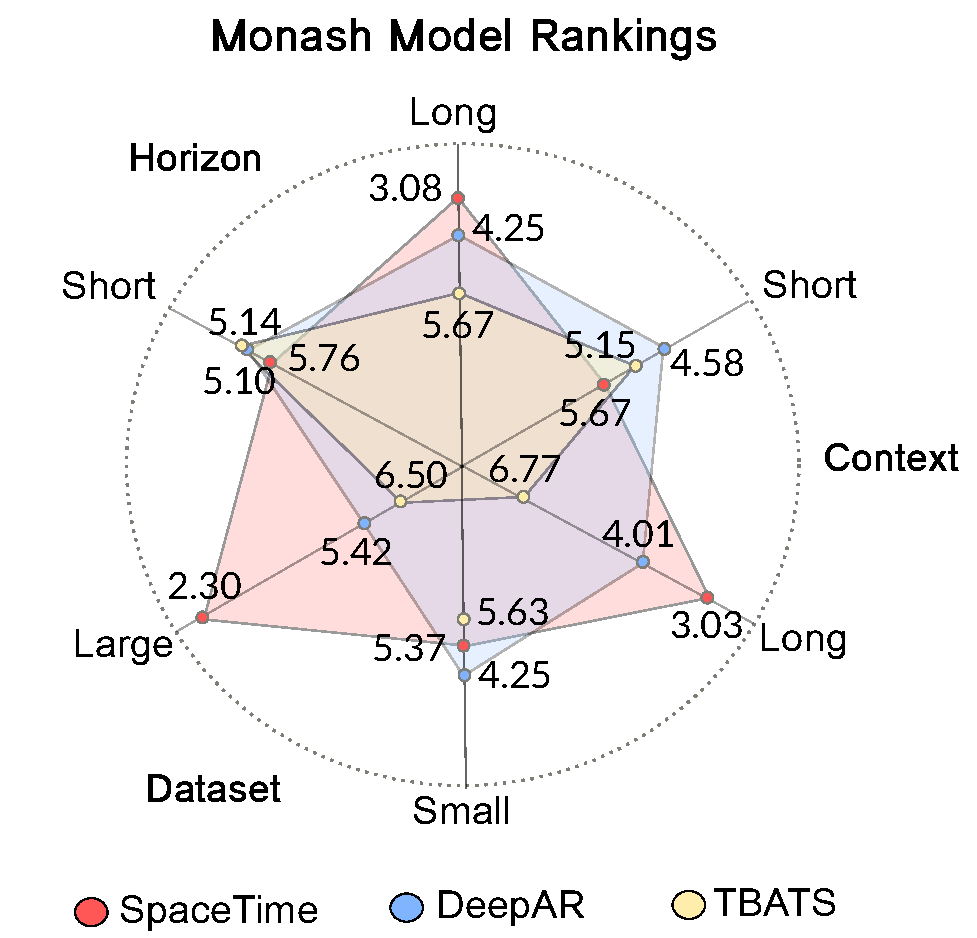
\includegraphics[width=0.5\linewidth]{_ICLR2023_paper/figures/monash_rankings2.pdf}
    \caption{ Relative test RMSE rankings ($*/13$ models) across different slices of the $33$ datasets in the Monash repository \citep{godahewa2021monash}. \ourmethod{} sets best overall ranking across all tasks and is significantly more accurate on tasks involving long forecast horizon and larger number of training samples.}
    \label{fig:monash_rankings}
\end{figure}
%\end{wrapfigure}


\subsection{ECG Classification}\label{appendix:ecg_results}

In addition to our results table in the main paper, we also provide the mean and standard deviations of the two models we ran in house (\ourmethod{} and S4) in Table \ref{tab:ecg_stats}.

\begin{table}[H]
    \centering
    \caption{ \textbf{ECG statement classification} on PTB-XL (100 Hz version). We report the mean and standard deviation over three random seeds for the three methods we ran in house.}
    \label{tab:ecg_stats}
    \begin{tabular}{@{}lcccccc@{}}
\toprule
Task AUROC & All            & Diag           & Sub-diag       & Super-diag     & Form           & Rhythm         \\ \midrule
\ourmethod{}            & $93.6 (0.13)$   & $94.1 (0.12)$ & $93.3(0.34)$ & $92.9 (0.09)$ & $88.3(0.63)$          & $96.7 (0.05)$    \\
S4    & $93.8 (0.38)$ & $93.9 (0.15)$  & $92.9 (0.11)$ & $93.1 (0.07)$    & $89.5 (0.66)$  & $97.7 (0.04)$ \\
Transformer    & $85.7 (0.30)$ & $87.6 (0.41)$  & $88.2 (0.20)$ & $88.7 (0.28)$    & $77.1 (0.45)$  & $83.1 (0.72)$ \\
\bottomrule
\end{tabular}
    
\end{table}


\subsection{Efficiency Results}

We additionally empirically validate that \ourmethod{} trains in near-linear time with horizon sequence length. We also use synthetic data, scaling horizon from $1 - 1000$. 

\begin{figure}[H]
  \centering
    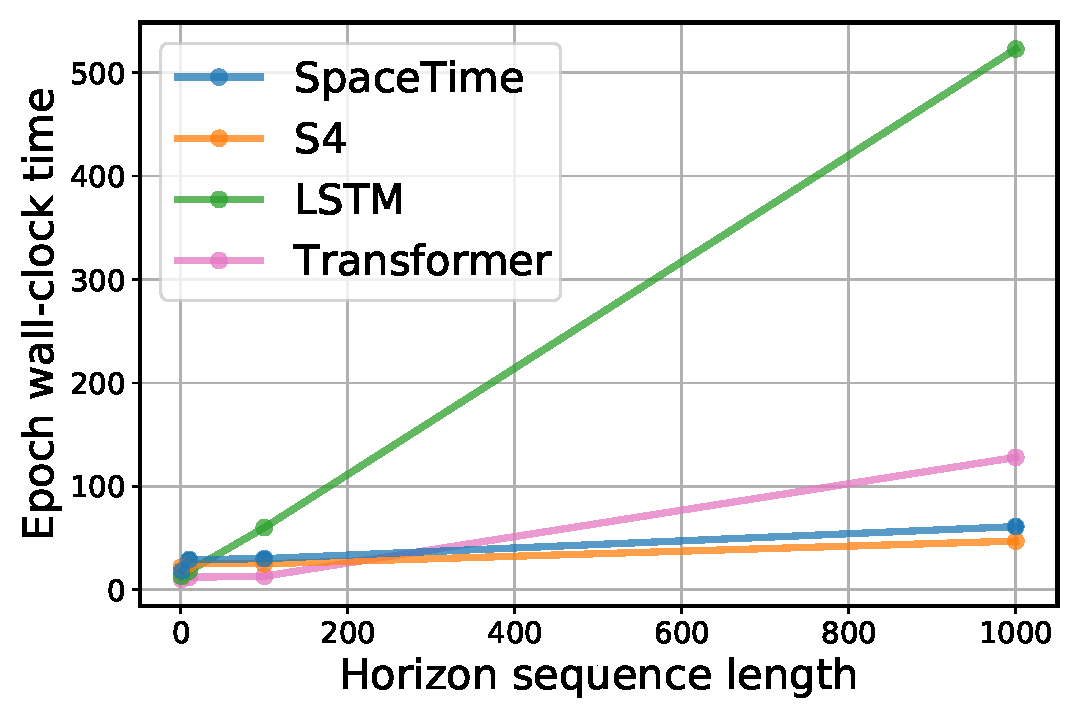
\includegraphics[width=0.5\textwidth]{_ICLR2023_paper/figures/speed_benchmark_horizon.pdf}
  \caption{Training wall-clock time versus horizon length for \ourmethod{}, S4, LSTM, and Transformer. }
  \label{fig:horizon_efficiency} 
\end{figure}


\subsection{\ourmethod{} Ablations}\label{appendix:ablations}
To better understand how the proposed \ourmethod{} SSMs lead to the improved empirical performance, we include ablations on the individual closed-loop forecasting SSM (Section~\ref{sec:forecasting_ssm}) and preprocessing SSMs (Section~\ref{sec:preprocessing_ssms}). 

\subsubsection{Closed-loop Forecasting SSM}\label{appendix:ablations_closed_loop_ssm}
To study how the closed-loop SSM improves long horizon forecasting accuracy, we remove the closed-loop SSM component in our default \ourmethod{} forecasting architecture (\cf{} Appendix~\ref{appendix:architectures}, and compare the default \ourmethod{} with one without any closed-loop SSMs on Informer forecasting tasks. For models without closed-loop SSMs, we replace the last layer with the standard ``open-loop'' SSM framework in Section~\ref{sec:method_spacetime_layer}), and keep all other layers the same. Finally, for baseline comparison against another SSM without the closed-loop component, we compare against S4. 

In Table~\ref{tab:ablation_results_closed_loop_ssm}, we report standardized MSE on Informer ETT datasets. Adding the closed-loop SSM consistently improves forecasting accuracy, on average lowering relative MSE by 33.2\%. Meanwhile, even without the closed-loop SSM, \ourmethod{} outperforms S4, again suggesting that the companion matrix parameterization is beneficial for autoregressive time series forecasting. 

\begin{table}[H]
    \centering
    \caption{ \textbf{Closed-loop SSM Ablation} We ablate the closed-loop SSM component in \ourmethod{}, comparing against the prior S4 SSM on four Informer time series forecasting tasks. Removing the closed-loop SSM consistently hurts forecasting accuracy for \ourmethod{}. }
    \label{tab:ablation_results_closed_loop_ssm}
    \begin{tabular}{@{}lbcbcbcbc@{}}
\toprule
                            & \multicolumn{2}{c}{ETTh1 (720)} & \multicolumn{2}{c}{ETTh2 (720)} & \multicolumn{2}{c}{ETTm1 (720)} & \multicolumn{2}{c}{ETTm2 (720)} \\ \cmidrule(l){2-9} 
Method / Ablation                      & MSE            & MAE            & MSE            & MAE            & MSE            & MAE            & MSE            & MAE            \\ \midrule
\ourmethod{}                & 0.076          & 0.222          & 0.188          & 0.352          & 0.074          & 0.213          & 0.166          & 0.318          \\
\ourmethod{} No Closed-loop & 0.114          & 0.271          & 0.278          & 0.431          & 0.156          & 0.310          & 0.213          & 0.365          \\
S4 (No Closed-loop)         & 0.190          & 0.355          & 0.630          & 0.662          & 0.254          & 0.433          & 0.482          & 0.567          \\ \bottomrule
\end{tabular}
    
\end{table}

\subsubsection{Preprocessing SSM}\label{appendix:ablations_preprocessing_ssm}

To study how the preprocessing SSM improves long horizon forecasting accuracy, we next compare how \ourmethod{} performs with and without the weight-initializing preprocessing SSMs introduced in Section~\ref{sec:preprocessing_ssms}. We compare the default \ourmethod{} architecture (Table~\ref{tab:spacetime_forecasting_arch} with (1) replacing the preprocessing SSMs with randomly initialized default companion SSMs, and (2) removing the preprocessing SSMs altogether. For the former, we preserve the number of layers, but now train the first-layer SSM weights. For the latter, there is one-less layer, but the same number of trainable parameters (as we fix and freeze the weights for each preprocessing SSM). 


In Table~\ref{tab:ablation_results_preprocessing_ssm}, we report standardized MSE on Informer ETT datasets. We find fixing the first layer SSMs of a \ourmethod{} network to preprocessing SSMs consistently improves forecasting performance, achieving 4.55\% lower MSE on average than the ablation with just trainable companion matrices. Including the preprocessing layer also improves MSE by 9.26\% on average compared to removing the layer altogether. These results suggest that preprocessing SSMs are beneficial for time series forecasting, \eg{} by performing classic time series modeling techniques on input data. Unlike other approaches, \ourmethod{} is able to flexibly and naturally incorporate these operations into its network layers via simple weight initializations of the same general companion SSM structure. 


\begin{table}[H]
    \centering
    \caption{ \textbf{Preprocessing SSM Ablation} We ablate the preprocessing SSM layer in \ourmethod{}, comparing against either replacing the SSMs with companion SSMs (Companion) or removing the layer (Removed). Including preprocessing SSMs consistently improves forecasting accuracy. }
    \label{tab:ablation_results_preprocessing_ssm}
\resizebox{\linewidth}{!}{
\begin{tabular}{@{}lbcbcbcbc@{}}
\toprule
                                           & \multicolumn{2}{c}{ETTh1 (720)} & \multicolumn{2}{c}{ETTh2 (720)} & \multicolumn{2}{c}{ETTm1 (720)} & \multicolumn{2}{c}{ETTm2 (720)} \\ \cmidrule(l){2-9} 
Method / Ablation                          & MSE            & MAE            & MSE            & MAE            & MSE            & MAE            & MSE            & MAE            \\ \midrule
SpaceTime                                  & 0.076          & 0.222          & 0.188          & 0.352          & 0.074          & 0.213          & 0.166          & 0.318          \\
SpaceTime No Preprocessing (Companion)     & 0.076          & 0.224          & 0.194          & 0.358          & 0.079          & 0.218          & 0.182          & 0.336          \\
SpaceTime No Preprocessing (Removed) & 0.078          & 0.227          & 0.204          & 0.367          & 0.087          & 0.232          & 0.188          & 0.326          \\ \bottomrule
\end{tabular}
}    
\end{table}


\subsection{\ourmethod{} Architectures}\label{appendix:architectures}

We provide the specific \ourmethod{} architecture configurations used for forecasting and classification tasks. Each configuration follows the general architecture presented in Section~\ref{sec:expressive_ssm_layer} and Figure~\ref{fig:arch_overview}, and consists of repeated Multi-SSM \ourmethod{} layers. We first provide additional details on specific instantiations of the companion SSMs we use in our models, \eg{} how we instantiate preprocessing SSMs to recover specific techniques (Section~\ref{sec:preprocessing_ssms}). We then include the layer-specific details of the number and type of SSM used in each network. 

\subsubsection{Specific SSM parameterizations}\label{appendix:specific_ssm_parameterizations}
In Section~\ref{sec:expressive_ssm_with_companion}, we described the general form of the companion SSM used in this work. By default, for any individual SSM we learn the $a$ column in $\zA$ and the vectors $\zB, \zC$ as trainable parameters in a neural net module. We refer to these SSMs specifically as \textbf{companion SSMs}. 

In addition, as discussed in Sections~\ref{sec:expressive_ssm_with_companion} and ~\ref{sec:preprocessing_ssms}, we can also fix $a$, $\zB$, or $\zC$ to specific values to recover useful operations when computing the SSM outputs. We describe specific instantiations of the companion SSM used in our models below (with dimensionality referring to one SSM). 

\header{Shift SSM}
We fix the $\boldsymbol{a}$ vector in the companion state matrix $\zA \in \mathbb{R}^{d \times d}$ to the $\boldsymbol{0}$ vector $\in \mathbb{R}^d$, such that $\zA$ is the shift matrix (see Eq.~\ref{eq:shift_matrix_example} for an example). This is a generalization of a 1-D ``sliding window'' convolution with fixed kernel size equal to SSM state dimension $d$. To see how, note that if $\zB$ is also fixed to the first basis vector $\boldsymbol{e_1} \in \mathbb{R}^{d \times 1}$, then this exactly recovers a 1-D convolution with kernel determined by $\zC$.

\header{Differencing SSM}
As a specific version of the preprocessing SSM discussed in Section~\ref{sec:preprocessing_ssms}, we fix $\boldsymbol{a} = \boldsymbol{0}$, $\zB = \boldsymbol{e_1}$, and set $\zC$ to recover various order differencing when computing the SSM, \ie{}
% \begin{align}
% \zC = \bmatrix 1 & -1 & 0 & \ldots & 0}\;\;\;\text{(1st-order differencing)}
% \end{align}
\begin{align}
    \zC &= 
    \begin{bmatrix}
    1 & \phantom{-}0 & 0 & \phantom{-}0 & 0 & \ldots & 0 \\
    \end{bmatrix}
    \;\;\;\;\;\;
    \begin{matrix}
    \hfill\text{(0-order differencing, \ie{} an identity function)} \\
    \end{matrix} \\
    \zC &= 
    \begin{bmatrix}
    1 & -1 & 0 & \phantom{-}0 & 0 & \ldots & 0 \\
    \end{bmatrix}
    \;\;\;\;\;\;
    \begin{matrix}
    \hfill\text{(1st-order differencing)} \\
    \end{matrix} \\
    \zC &= 
    \begin{bmatrix}
    1 & -2 & 1 & \phantom{-}0 & 0 & \ldots & 0 \\
    \end{bmatrix}
    \;\;\;\;\;\;
    \begin{matrix}
    \hfill\text{ (2nd-order differencing)} \\
    \end{matrix} \\
    \zC &= 
    \begin{bmatrix}
    1 & -3 & 3 & -1 & 0 & \ldots & 0 \\
    \end{bmatrix}
    \;\;\;\;\;\;
    \begin{matrix}
    \hfill\text{ (3rd-order differencing)} \\
    \end{matrix}
\end{align}
 In this work, we only use the above 0, 1st, 2nd, or 3rd-order differencing instantiations. With multiple differencing SSMs in a multi-SSM \ourmethod{} layer, we initialize differencing SSMs by running through the orders repeatedly in sequence. For example, given five differencing SSMs, the first four SSMs perform 0, 1st, 2nd, and 3rd-order differencing respectively, while the fifth performs 0-order differencing again.

\header{Moving Average Residual (MA residual) SSM}
As another version of the preprocessing SSM, we can fix $\boldsymbol{a} = \boldsymbol{0}$, $\zB = \boldsymbol{e_1}$, and set $\zC$ such that the SSM outputs sample residuals from a moving average applied over the input sequence. For an $n$-order moving average, we compute outputs with $\zC$ specified as
\begin{align}
    \zC &= 
    \begin{bmatrix}
    1 - 1/n, & -1/n, & \ldots & -1/n, & 0 & \ldots & 0 \\
    \end{bmatrix}
    \;\;\;\;\;\;
    \begin{matrix}
    \hfill\text{($n$-order moving average residual)} \\
    \end{matrix}
\end{align}
For each MA residual SSM, we randomly initialize the order by uniform-randomly sampling an integer in the range $[4, d]$, where $d$ is again the state-space dimension size (recall $\zC \in \mathbb{R}^{1 \times d}$). We pick $4$ as a heuristic which was not finetuned; we leave additional optimization here for further work.

\subsubsection{Task-specific \ourmethod{} Architectures}\label{appendix:specific_spacetime_architectures}

Here we provide layer-level details on the \ourmethod{} networks used in this work. For each task, we describe number of layers, number of SSMs per layer, state-space dimension (fixed for all SSMs in a network), and which SSMs are used in each layer. 

Expanding on this last detail, as previously discussed in Section~\ref{sec:method_spacetime_layer}, in each \ourmethod{} layer we can specify multiple SSMs in each layer, computing their outputs in parallel to produce a multidimensional output that is fed as the input to the next \ourmethod{} layer. The ``types'' of SSMs do not all have to be the same per layer, and we list the type (companion, shift, differencing, MA residual) and closed-loop designation (standard, closed-loop) of the SSMs in each layer below.

For an additional visual overview of a \ourmethod{} network, please refer back to Figure~\ref{fig:arch_overview}.

\header{Forecasting: Informer and Monash}
We describe the architecture in Table~\ref{tab:spacetime_forecasting_arch}. We treat the first \ourmethod{} layer as ``preprocessing'' layer, which performs differencing and moving average residual operations on the input sequence. We treat the last \ourmethod{} layer as a ``forecasting'' layer, which autoregressively outputs future horizon predictions given the second-to-last layer's outputs as an input sequence.

% \[
% \begin{aligned}
%     \begin{matrix}
%     \text{\phantom{-}} \\
%     \end{matrix}
%     \\
%     &
%     \begin{bmatrix}
%     \text{\phantom{-} Differencing \phantom{-}}   \\ \text{(standard)} \\
%     \end{bmatrix}
%     \times 192 
%     \\
%     \begin{matrix}
%     \text{\phantom{-}} \\
%     \end{matrix}
%     \\
%     &
%     &
%     \begin{bmatrix}
%     \text{\phantom{-} MA Residual\phantom{-} }   \\ \text{(standard)} \\
%     \end{bmatrix}
%      \times 64 
%      \\
%      \begin{matrix}
%     \text{\phantom{-}} \\
%     \end{matrix}
%     \\
% \end{aligned}
% \]

% \[
% \begin{aligned}
%     \begin{matrix}
%     \text{\phantom{-}} \\
%     \end{matrix}
%     \\
%     &
%     \begin{bmatrix}
%     \text{\phantom{-} Differencing \phantom{-}}   \\ \text{(standard)} \\
%     \end{bmatrix}
%     \times 256 
%     \\
%      \begin{matrix}
%     \text{\phantom{-}} \\
%     \end{matrix}
%     \\
% \end{aligned}
% \]


% \[
% \begin{aligned}
%     \begin{matrix}
%     \text{\phantom{-}} \\
%     \end{matrix}
%     \\
%     &
%     \begin{bmatrix}
%     \text{\phantom{-} Differencing \phantom{-}}   \\ \text{(standard)} \\
%     \end{bmatrix}
%     \times 192 
%     \\
%      \begin{matrix}
%     \text{\phantom{-}} \\
%     \end{matrix}
%     \\
% \end{aligned}
% \]

% \[
% \begin{aligned}
%     \begin{matrix}
%     \text{\phantom{-}} \\
%     \end{matrix}
%     \\
%     \begin{bmatrix}
%     \text{\phantom{-} Companion \phantom{-}}   \\ \text{(standard)} \\
%     \end{bmatrix}
%     \times 256 
%     \\
%     \begin{matrix}
%     \text{\phantom{-}} \\
%     \end{matrix}
%     \\
% \end{aligned}
% \]


% \[
% \begin{aligned}
%     \begin{matrix}
%     \text{\phantom{-}} \\
%     \end{matrix}
%     \\
%     \begin{bmatrix}
%     \text{\phantom{-} Shift \phantom{-}}   \\ \text{(standard)} \\
%     \end{bmatrix}
%     \times 256 
%     \\
%     \begin{matrix}
%     \text{\phantom{-}} \\
%     \end{matrix}
%     \\
% \end{aligned}
% \]


% \[
% \begin{aligned}
%     \begin{matrix}
%     \text{\phantom{-}} \\
%     \end{matrix}
%     \\
%     &
%     \begin{bmatrix}
%     \text{\phantom{-} Companion \phantom{-}}   \\ \text{(standard)} \\
%     \end{bmatrix}
%     \times 128 
%     \\
%     \begin{matrix}
%     \text{\phantom{-}} \\
%     \end{matrix}
%     \\
%     &
%     &
%     \begin{bmatrix}
%     \text{\phantom{-} Shift \phantom{-} }   \\ \text{(standard)} \\
%     \end{bmatrix}
%      \times 128  
%      \\
%      \begin{matrix}
%     \text{\phantom{-}} \\
%     \end{matrix}
%     \\
% \end{aligned}
% \]

% \[
% \begin{aligned}
%     \begin{matrix}
%     \text{\phantom{-}} \\
%     \end{matrix}
%     \\
%     \begin{bmatrix}
%     \text{\phantom{-} Companion \phantom{-} }   \\ \text{(closed-loop)} \\
%     \end{bmatrix}
%     \times 128 
%     \\
%     \begin{matrix}
%     \text{\phantom{-}} \\
%     \end{matrix}
%     \\
% \end{aligned}
% \]


\header{Classification: ECG}
We describe the architectures for each ECG classification task in Tables~\ref{tab:spacetime_ecg_superdiag}--\ref{tab:spacetime_ecg_all}. For all models, we use state-space dimension $d = 64$. As described in the experiments, for classification we compute logits with a mean pooling over the output sequence, where pooling is computed over the sequence length. 

\header{Classification: Speech Audio}
We describe the architecture for the Speech Audio task in Table~\ref{tab:spacetime_speech}. We use state-space dimension $d = 1024$. As described in the experiments, for classification we compute logits with a mean pooling over the output sequence, where pooling is computed over the sequence length. 


\begin{table}[]
\centering
\caption{\ourmethod{} forecasting architecture. For all SSMs, we keep state-space dimension $d = 128$. Repeated Identity denotes repeating the input to match the number of SSMs in the next layer, \ie{} 128 SSMs in this case. For each forecasting task, $d'$ denotes time series samples' number of features, $\ell$ denotes the lag size (number of past samples given as input), and $h$ denotes the horizon size (number of future samples to be predicted).}
\label{tab:spacetime_forecasting_arch}
\begin{tabular}{@{}c|c|c|c@{}}
Layer                             & Details                                                                                                                                                                                                                                                                                                                                                                                                                                                                                     & Input Size        & Output Size       \\ \midrule
\multicolumn{1}{c|}{Decoder}     & Linear                                                                                                                                                                                                                                                                                                                                                                                                                                                                                     & $128 \times \ell$ &  $d' \times h$   \\ \midrule
\multicolumn{1}{c|}{SSM Layer 3} & \begin{math}\begin{aligned}    \begin{matrix}    \text{\phantom{-}} \\    \end{matrix}    \\    \begin{bmatrix}    \text{\phantom{-} Companion \phantom{-} } \\ \text{(closed-loop)} \\    \end{bmatrix}    \times 128     \\    \begin{matrix}    \text{\phantom{-}} \\    \end{matrix}    \\\end{aligned}\end{math}                                                                                                                                                                        & $128 \times \ell$ & $128 \times \ell$ \\ \midrule
\multicolumn{1}{c|}{SSM Layer 2} & \begin{math}\begin{aligned}    \begin{matrix}    \text{\phantom{-}} \\    \end{matrix}    \\    \begin{bmatrix}    \text{\phantom{-} Companion \phantom{-}}  \\ \text{(standard)} \\    \end{bmatrix}    \times 128     \\    \begin{matrix}    \text{\phantom{-}} \\    \end{matrix}    \\\end{aligned}\end{math}                                                                                                                                                                             & $128 \times \ell$ & $128 \times \ell$ \\ \midrule
\multicolumn{1}{c|}{\text{SSM Layer 1}} & \begin{math}\begin{aligned}    \begin{matrix}    \text{\phantom{-}} \\    \end{matrix}    \\    &    \begin{bmatrix}    \text{\phantom{-} Differencing \phantom{-}}  \\ \text{(standard)} \\    \end{bmatrix}    \times 64     \\    \begin{matrix}    \text{\phantom{-}} \\    \end{matrix}    \\    &    \begin{bmatrix}    \text{\phantom{-} MA Residual\phantom{-} }  \\ \text{(standard)} \\    \end{bmatrix}     \times 64      \\     \begin{matrix}    \text{\phantom{-}} \\    \end{matrix}    \\\end{aligned}\end{math} & $128 \times \ell$ & $128 \times \ell$ \\ \midrule
\multicolumn{1}{c|}{Encoder}     & Repeated Identity                                                                                                                                                                                                                                                                                                                                                                                                                                                                                   & $d' \times \ell$   & $128 \times \ell$ \\ \bottomrule
\end{tabular}
\end{table}


\begin{table}[]
\centering
\caption{\ourmethod{} architecture for ECG SuperDiagnostic classification. For all SSMs, we keep state-space dimension $d = 64$. Input samples have $d' = 12$ features and are length $\ell = 1000$ time-steps long. The number of classes $c = 5$.}
\label{tab:spacetime_ecg_superdiag}
\begin{tabular}{@{}c|c|c|c@{}}
Layer       & Details                                                                                                                                                                                                                                                                                                                 & Input Size        & Output Size       \\ \midrule
Classifier  & Mean Pooling                                                                                                                                                                                                                                                                                                            & $c \times \ell$   & $c \times 1$      \\ \midrule
Decoder     & Linear                                                                                                                                                                                                                                                                                                                  & $256 \times \ell$ & $c \times \ell$   \\ \midrule
SSM Layer 5 & \begin{math}\begin{aligned}    \begin{matrix}    \text{\phantom{-}} \\    \end{matrix}    \\    \begin{bmatrix}    \text{\phantom{-} Companion \phantom{-}}  \\ \text{(standard)} \\    \end{bmatrix}    \times 256     \\    \begin{matrix}    \text{\phantom{-}} \\    \end{matrix}    \\\end{aligned}\end{math}          & $256 \times \ell$ & $256 \times \ell$ \\ \midrule
SSM Layer 4 & \begin{math}\begin{aligned}    \begin{matrix}    \text{\phantom{-}} \\    \end{matrix}    \\    \begin{bmatrix}    \text{\phantom{-} Companion \phantom{-}} \\ \text{(standard)} \\    \end{bmatrix}    \times 256     \\    \begin{matrix}    \text{\phantom{-}} \\    \end{matrix}    \\\end{aligned}\end{math}          & $256 \times \ell$ & $256 \times \ell$ \\ \midrule
SSM Layer 3 & \begin{math}\begin{aligned}    \begin{matrix}    \text{\phantom{-}} \\    \end{matrix}    \\    \begin{bmatrix}    \text{\phantom{-} Companion \phantom{-}} \\ \text{(standard)} \\    \end{bmatrix}    \times 256     \\    \begin{matrix}    \text{\phantom{-}} \\    \end{matrix}    \\\end{aligned}\end{math}          & $256 \times \ell$ & $256 \times \ell$ \\ \midrule
SSM Layer 2 & \begin{math}\begin{aligned}    \begin{matrix}    \text{\phantom{-}} \\    \end{matrix}    \\    \begin{bmatrix}    \text{\phantom{-} Companion \phantom{-}} \\ \text{(standard)} \\    \end{bmatrix}    \times 256     \\    \begin{matrix}    \text{\phantom{-}} \\    \end{matrix}    \\\end{aligned}\end{math}          & $256 \times \ell$ & $256 \times \ell$ \\ \midrule
SSM Layer 1 & \begin{math}\begin{aligned}    \begin{matrix}    \text{\phantom{-}} \\    \end{matrix}    \\    &    \begin{bmatrix}    \text{\phantom{-} Differencing \phantom{-}} \\ \text{(standard)} \\    \end{bmatrix}    \times 256     \\     \begin{matrix}    \text{\phantom{-}} \\    \end{matrix}    \\\end{aligned}\end{math} & 256 $\times \ell$ & 256 $\times \ell$ \\ \midrule
Encoder     & Linear & $d' \times \ell$  & $256 \times \ell$ \\ \bottomrule
\end{tabular}
\end{table}

\begin{table}[]
\centering
\caption{\ourmethod{} architecture for ECG SubDiagnostic classification. For all SSMs, we keep state-space dimension $d = 64$. Input samples have $d' = 12$ features and are length $\ell = 1000$ time-steps long. The number of classes $c = 23$.}
\label{tab:spacetime_ecg_subdiag}
\begin{tabular}{@{}c|c|c|c@{}}
Layer       & Details                                                                                                                                                                                                                                                                                                                 & Input Size        & Output Size       \\ \midrule
Classifier  & Mean Pooling                                                                                                                                                                                                                                                                                                            & $c \times \ell$   & $c \times 1$      \\ \midrule
Decoder     & Linear                                                                                                                                                                                                                                                                                                                  & $256 \times \ell$ & $c \times \ell$   \\ \midrule
SSM Layer 5 & \begin{math}\begin{aligned}    \begin{matrix}    \text{\phantom{-}} \\    \end{matrix}    \\    \begin{bmatrix}    \text{\phantom{-} Shift \phantom{-}} \\ \text{(standard)} \\    \end{bmatrix}    \times 256     \\    \begin{matrix}    \text{\phantom{-}} \\    \end{matrix}    \\\end{aligned}\end{math}              & $256 \times \ell$ & $256 \times \ell$ \\ \midrule
SSM Layer 4 & \begin{math}\begin{aligned}    \begin{matrix}    \text{\phantom{-}} \\    \end{matrix}    \\    \begin{bmatrix}    \text{\phantom{-} Shift \phantom{-}}  \\ \text{(standard)} \\    \end{bmatrix}    \times 256     \\    \begin{matrix}    \text{\phantom{-}} \\    \end{matrix}    \\\end{aligned}\end{math}              & $256 \times \ell$ & $256 \times \ell$ \\ \midrule
SSM Layer 3 & \begin{math}\begin{aligned}    \begin{matrix}    \text{\phantom{-}} \\    \end{matrix}    \\    \begin{bmatrix}    \text{\phantom{-} Shift \phantom{-}} \\ \text{(standard)} \\    \end{bmatrix}    \times 256     \\    \begin{matrix}    \text{\phantom{-}} \\    \end{matrix}    \\\end{aligned}\end{math}              & $256 \times \ell$ & $256 \times \ell$ \\ \midrule
SSM Layer 2 & \begin{math}\begin{aligned}    \begin{matrix}    \text{\phantom{-}} \\    \end{matrix}    \\    \begin{bmatrix}    \text{\phantom{-} Shift \phantom{-}} \\ \text{(standard)} \\    \end{bmatrix}    \times 256     \\    \begin{matrix}    \text{\phantom{-}} \\    \end{matrix}    \\\end{aligned}\end{math}              & $256 \times \ell$ & $256 \times \ell$ \\ \midrule
SSM Layer 1 & \begin{math}\begin{aligned}    \begin{matrix}    \text{\phantom{-}} \\    \end{matrix}    \\    &    \begin{bmatrix}    \text{\phantom{-} Differencing \phantom{-}} \\ \text{(standard)} \\    \end{bmatrix}    \times 256     \\     \begin{matrix}    \text{\phantom{-}} \\    \end{matrix}    \\\end{aligned}\end{math} & $256 \times \ell$ & $256 \times \ell$ \\ \midrule
Encoder     & Linear                                                                                                                                                                                                                                                                                                                  & $d' \times \ell$  & $256 \times \ell$ \\ \bottomrule
\end{tabular}
\end{table}

\begin{table}[]
\centering
\caption{\ourmethod{} architecture for ECG Diagnostic classification. For all SSMs, we keep state-space dimension $d = 64$. Input samples have $d' = 12$ features and are length $\ell = 1000$ time-steps long. The number of classes $c = 44$.}
\label{tab:spacetime_ecg_diag}
\begin{tabular}{@{}c|c|c|c@{}}
Layer       & Details                                                                                                                                                                                                                                                                                                                 & Input Size        & Output Size       \\ \midrule
Classifier  & Mean Pooling                                                                                                                                                                                                                                                                                                            & $c \times \ell$   & $c \times 1$      \\ \midrule
Decoder     & Linear                                                                                                                                                                                                                                                                                                                  & $256 \times \ell$ & $c \times \ell$   \\ \midrule
SSM Layer 5 & \begin{math}\begin{aligned}    \begin{matrix}    \text{\phantom{-}} \\    \end{matrix}    \\    \begin{bmatrix}    \text{\phantom{-} Shift \phantom{-}} \\ \text{(standard)} \\    \end{bmatrix}    \times 256     \\    \begin{matrix}    \text{\phantom{-}} \\    \end{matrix}    \\\end{aligned}\end{math}              & $256 \times \ell$ & $256 \times \ell$ \\ \midrule
SSM Layer 4 & \begin{math}\begin{aligned}    \begin{matrix}    \text{\phantom{-}} \\    \end{matrix}    \\    \begin{bmatrix}    \text{\phantom{-} Shift \phantom{-}}  \\ \text{(standard)} \\    \end{bmatrix}    \times 256     \\    \begin{matrix}    \text{\phantom{-}} \\    \end{matrix}    \\\end{aligned}\end{math}              & $256 \times \ell$ & $256 \times \ell$ \\ \midrule
SSM Layer 3 & \begin{math}\begin{aligned}    \begin{matrix}    \text{\phantom{-}} \\    \end{matrix}    \\    \begin{bmatrix}    \text{\phantom{-} Shift \phantom{-}}  \\ \text{(standard)} \\    \end{bmatrix}    \times 256     \\    \begin{matrix}    \text{\phantom{-}} \\    \end{matrix}    \\\end{aligned}\end{math}              & $256 \times \ell$ & $256 \times \ell$ \\ \midrule
SSM Layer 2 & \begin{math}\begin{aligned}    \begin{matrix}    \text{\phantom{-}} \\    \end{matrix}    \\    \begin{bmatrix}    \text{\phantom{-} Shift \phantom{-}} \\ \text{(standard)} \\    \end{bmatrix}    \times 256     \\    \begin{matrix}    \text{\phantom{-}} \\    \end{matrix}    \\\end{aligned}\end{math}              & $256 \times \ell$ & $256 \times \ell$ \\ \midrule
SSM Layer 1 & \begin{math}\begin{aligned}    \begin{matrix}    \text{\phantom{-}} \\    \end{matrix}    \\    &    \begin{bmatrix}    \text{\phantom{-} Differencing \phantom{-}} \\ \text{(standard)} \\    \end{bmatrix}    \times 256     \\     \begin{matrix}    \text{\phantom{-}} \\    \end{matrix}    \\\end{aligned}\end{math} & $256 \times \ell$ & $256 \times \ell$ \\ \midrule
Encoder     & Linear                                                                                                                                                                                                                                                                                                                  & $d' \times \ell$  & $256 \times \ell$ \\ \bottomrule
\end{tabular}
\end{table}


\begin{table}[]
\centering
\caption{\ourmethod{} architecture for ECG Form classification. For all SSMs, we keep state-space dimension $d = 64$. Input samples have $d' = 12$ features and are length $\ell = 1000$ time-steps long. The number of classes $c = 19$.}
\label{tab:spacetime_ecg_form}
\begin{tabular}{@{}c|c|c|c@{}}
Layer       & Details                                                                                                                                                                                                                                                                                                                                                                                                                                                                                                                                      & Input Size        & Output Size       \\ \midrule
Classifier  & Mean Pooling                                                                                                                                                                                                                                                                                                                                                                                                                                                                                                                                 & $c \times \ell$   & $c \times 1$      \\ \midrule
Decoder     & Linear                                                                                                                                                                                                                                                                                                                                                                                                                                                                                                                                       & $256 \times \ell$ & $c \times \ell$   \\ \midrule
SSM Layer 5 & \begin{math}\begin{aligned}    \begin{matrix}    \text{\phantom{-}} \\    \end{matrix}    \\    \begin{bmatrix}    \text{\phantom{-} Companion \phantom{-}}  \\ \text{(standard)} \\    \end{bmatrix}    \times 256     \\    \begin{matrix}    \text{\phantom{-}} \\    \end{matrix}    \\\end{aligned}\end{math}                                                                                                                                                                                                                               & $256 \times \ell$ & $256 \times \ell$ \\ \midrule
SSM Layer 4 & \begin{math}\begin{aligned}    \begin{matrix}    \text{\phantom{-}} \\    \end{matrix}    \\    \begin{bmatrix}    \text{\phantom{-} Companion \phantom{-}}   \\ \text{(standard)} \\    \end{bmatrix}    \times 256     \\    \begin{matrix}    \text{\phantom{-}} \\    \end{matrix}    \\\end{aligned}\end{math}                                                                                                                                                                                                                               & $256 \times \ell$ & $256 \times \ell$ \\ \midrule
SSM Layer 3 & \begin{math}\begin{aligned}    \begin{matrix}    \text{\phantom{-}} \\    \end{matrix}    \\    \begin{bmatrix}    \text{\phantom{-} Companion \phantom{-}}   \\ \text{(standard)} \\    \end{bmatrix}    \times 256     \\    \begin{matrix}    \text{\phantom{-}} \\    \end{matrix}    \\\end{aligned}\end{math}                                                                                                                                                                                                                               & $256 \times \ell$ & $256 \times \ell$ \\ \midrule
SSM Layer 2 & \begin{math}\begin{aligned}    \begin{matrix}    \text{\phantom{-}} \\    \end{matrix}    \\    \begin{bmatrix}    \text{\phantom{-} Companion \phantom{-}}   \\ \text{(standard)} \\    \end{bmatrix}    \times 256     \\    \begin{matrix}    \text{\phantom{-}} \\    \end{matrix}    \\\end{aligned}\end{math}                                                                                                                                                                                                                               & $256 \times \ell$ & $256 \times \ell$ \\ \midrule
SSM Layer 1 & \begin{math}\begin{aligned}    \begin{matrix}    \text{\phantom{-}} \\    \end{matrix}    \\    &    \begin{bmatrix}    \text{\phantom{-} Differencing \phantom{-}}   \\ \text{(standard)} \\    \end{bmatrix}    \times 192     \\    \begin{matrix}    \text{\phantom{-}} \\    \end{matrix}    \\    &    \begin{bmatrix}    \text{\phantom{-} MA Residual\phantom{-} }   \\ \text{(standard)} \\    \end{bmatrix}     \times 64      \\     \begin{matrix}    \text{\phantom{-}} \\    \end{matrix}    \\\end{aligned}\end{math} & $256 \times \ell$ & $256 \times \ell$ \\ \midrule
Encoder     & Linear                                                                                                                                                                                                                                                                                                                                                                                                                                                                                                                                       & $d' \times \ell$  & $256 \times \ell$ \\ \bottomrule
\end{tabular}
\end{table}



\begin{table}[]
\centering
\caption{\ourmethod{} architecture for ECG Rhythm classification. For all SSMs, we keep state-space dimension $d = 64$. Input samples have $d' = 12$ features and are length $\ell = 1000$ time-steps long. The number of classes $c = 12$.}
\label{tab:spacetime_ecg_rhythm}
\begin{tabular}{@{}c|c|c|c@{}}
Layer       & Details                                                                                                                                                                                                                                                                                                                                                                                                                                                                                                                                & Input Size        & Output Size       \\ \midrule
Classifier  & Mean Pooling                                                                                                                                                                                                                                                                                                                                                                                                                                                                                                                           & $c \times \ell$   & $c \times 1$      \\ \midrule
Decoder     & Linear                                                                                                                                                                                                                                                                                                                                                                                                                                                                                                                                 & $256 \times \ell$ & $c \times \ell$   \\ \midrule
SSM Layer 5 & \begin{math}\begin{aligned}    \begin{matrix}    \text{\phantom{-}} \\    \end{matrix}    \\    &    \begin{bmatrix}    \text{\phantom{-} Companion \phantom{-}}   \\ \text{(standard)} \\    \end{bmatrix}    \times 128     \\    \begin{matrix}    \text{\phantom{-}} \\    \end{matrix}    \\    &    \begin{bmatrix}    \text{\phantom{-} Shift \phantom{-} }   \\ \text{(standard)} \\    \end{bmatrix}     \times 128       \\     \begin{matrix}    \text{\phantom{-}} \\    \end{matrix}    \\\end{aligned}\end{math} & $256 \times \ell$ & $256 \times \ell$ \\ \midrule
SSM Layer 4 & \begin{math}\begin{aligned}    \begin{matrix}    \text{\phantom{-}} \\    \end{matrix}    \\    &    \begin{bmatrix}    \text{\phantom{-} Companion \phantom{-}}   \\ \text{(standard)} \\    \end{bmatrix}    \times 128     \\    \begin{matrix}    \text{\phantom{-}} \\    \end{matrix}    \\    &    \begin{bmatrix}    \text{\phantom{-} Shift \phantom{-} }   \\ \text{(standard)} \\    \end{bmatrix}     \times 128       \\     \begin{matrix}    \text{\phantom{-}} \\    \end{matrix}    \\\end{aligned}\end{math} & $256 \times \ell$ & $256 \times \ell$ \\ \midrule
SSM Layer 3 & \begin{math}\begin{aligned}    \begin{matrix}    \text{\phantom{-}} \\    \end{matrix}    \\    &    \begin{bmatrix}    \text{\phantom{-} Companion \phantom{-}}   \\ \text{(standard)} \\    \end{bmatrix}    \times 128     \\    \begin{matrix}    \text{\phantom{-}} \\    \end{matrix}    \\    &    \begin{bmatrix}    \text{\phantom{-} Shift \phantom{-} }   \\ \text{(standard)} \\    \end{bmatrix}     \times 128       \\     \begin{matrix}    \text{\phantom{-}} \\    \end{matrix}    \\\end{aligned}\end{math} & $256 \times \ell$ & $256 \times \ell$ \\ \midrule
SSM Layer 2 & \begin{math}\begin{aligned}    \begin{matrix}    \text{\phantom{-}} \\    \end{matrix}    \\    &    \begin{bmatrix}    \text{\phantom{-} Companion \phantom{-}}   \\ \text{(standard)} \\    \end{bmatrix}    \times 128     \\    \begin{matrix}    \text{\phantom{-}} \\    \end{matrix}    \\    &    \begin{bmatrix}    \text{\phantom{-} Shift \phantom{-} }   \\ \text{(standard)} \\    \end{bmatrix}     \times 128       \\     \begin{matrix}    \text{\phantom{-}} \\    \end{matrix}    \\\end{aligned}\end{math} & $256 \times \ell$ & $256 \times \ell$ \\ \midrule
SSM Layer 1 & \begin{math}\begin{aligned}    \begin{matrix}    \text{\phantom{-}} \\    \end{matrix}    \\    &    \begin{bmatrix}    \text{\phantom{-} Differencing \phantom{-}}   \\ \text{(standard)} \\    \end{bmatrix}    \times 256     \\     \begin{matrix}    \text{\phantom{-}} \\    \end{matrix}    \\\end{aligned}\end{math}                                                                                                                                                                                                                & $256 \times \ell$ & $256 \times \ell$ \\ \midrule
Encoder     & Linear                                                                                                                                                                                                                                                                                                                                                                                                                                                                                                                                 & $d' \times \ell$  & $256 \times \ell$ \\ \bottomrule
\end{tabular}
\end{table}


\begin{table}[]
\centering
\caption{\ourmethod{} architecture for ECG All classification. For all SSMs, we keep state-space dimension $d = 64$. Input samples have $d' = 12$ features and are length $\ell = 1000$ time-steps long. The number of classes $c = 71$.}
\label{tab:spacetime_ecg_all}
\begin{tabular}{@{}c|c|c|c@{}}
Layer       & Details                                                                                                                                                                                                                                                                                                                                                                                                                                                                                                                                      & Input Size        & Output Size       \\ \midrule
Classifier  & Mean Pooling                                                                                                                                                                                                                                                                                                                                                                                                                                                                                                                                 & $c \times \ell$   & $c \times 1$      \\ \midrule
Decoder     & Linear                                                                                                                                                                                                                                                                                                                                                                                                                                                                                                                                       & $256 \times \ell$ & $c \times \ell$   \\ \midrule
SSM Layer 5 & \begin{math}\begin{aligned} \begin{matrix} \text{\phantom{-}} \\ \end{matrix} \\ \begin{bmatrix} \text{\phantom{-} Shift \phantom{-}}   \\ \text{(standard)} \\ \end{bmatrix} \times 256 \\ \begin{matrix} \text{\phantom{-}} \\ \end{matrix} \\\end{aligned}\end{math}                                                                                                                                                                                                                                                                           & $256 \times \ell$ & $256 \times \ell$ \\ \midrule
SSM Layer 4 & \begin{math}\begin{aligned} \begin{matrix} \text{\phantom{-}} \\ \end{matrix} \\ \begin{bmatrix} \text{\phantom{-} Shift \phantom{-}}   \\ \text{(standard)} \\ \end{bmatrix} \times 256 \\ \begin{matrix} \text{\phantom{-}} \\ \end{matrix} \\\end{aligned}\end{math}                                                                                                                                                                                                                                                                           & $256 \times \ell$ & $256 \times \ell$ \\ \midrule
SSM Layer 3 & \begin{math}\begin{aligned} \begin{matrix} \text{\phantom{-}} \\ \end{matrix} \\ \begin{bmatrix} \text{\phantom{-} Shift \phantom{-}}   \\ \text{(standard)} \\ \end{bmatrix} \times 256 \\ \begin{matrix} \text{\phantom{-}} \\ \end{matrix} \\\end{aligned}\end{math}                                                                                                                                                                                                                                                                           & $256 \times \ell$ & $256 \times \ell$ \\ \midrule
SSM Layer 2 & \begin{math}\begin{aligned}    \begin{matrix}    \text{\phantom{-}} \\    \end{matrix}    \\    \begin{bmatrix}    \text{\phantom{-} Shift \phantom{-}}   \\ \text{(standard)} \\    \end{bmatrix}    \times 256     \\    \begin{matrix}    \text{\phantom{-}} \\    \end{matrix}    \\\end{aligned}\end{math}                                                                                                                                                                                                                                   & $256 \times \ell$ & $256 \times \ell$ \\ \midrule
SSM Layer 1 & \begin{math}\begin{aligned}    \begin{matrix}    \text{\phantom{-}} \\    \end{matrix}    \\    &    \begin{bmatrix}    \text{\phantom{-} Differencing \phantom{-}}   \\ \text{(standard)} \\    \end{bmatrix}    \times 192     \\    \begin{matrix}    \text{\phantom{-}} \\    \end{matrix}    \\    &    \begin{bmatrix}    \text{\phantom{-} MA Residual\phantom{-} }   \\ \text{(standard)} \\    \end{bmatrix}     \times 64      \\     \begin{matrix}    \text{\phantom{-}} \\    \end{matrix}    \\\end{aligned}\end{math} & $256 \times \ell$ & $256 \times \ell$ \\ \midrule
Encoder     & Linear                                                                                                                                                                                                                                                                                                                                                                                                                                                                                                                                       & $d' \times \ell$  & $256 \times \ell$ \\ \bottomrule
\end{tabular}
\end{table}


\begin{table}[]
\centering
\caption{\ourmethod{} architecture for Speech Audio classification. For all SSMs, we keep state-space dimension $d = 1024$. Input samples have $d' = 1$ features and are length $\ell = 16000$ time-steps long. The number of classes $c = 10$.}
\label{tab:spacetime_speech}
\begin{tabular}{@{}c|c|c|c@{}}
Layer       & Details                                                                                                                                                                                                                                                                                                        & Input Size                              & Output Size                             \\ \midrule
Classifier  & Mean Pooling                                                                                                                                                                                                                                                                                                   & \cellcolor[HTML]{FFFFFF}$c \times \ell$ & $c \times 1$                            \\ \midrule
Decoder     & Linear                                                                                                                                                                                                                                                                                                         & $256 \times \ell$                       & \cellcolor[HTML]{FFFFFF}$c \times \ell$ \\ \midrule
SSM Layer 6 & \begin{math}\begin{aligned}    \begin{matrix}    \text{\phantom{-}} \\    \end{matrix}    \\    \begin{bmatrix}    \text{\phantom{-} Companion \phantom{-}}   \\ \text{(standard)} \\    \end{bmatrix}    \times 256     \\    \begin{matrix}    \text{\phantom{-}} \\    \end{matrix}    \\\end{aligned}\end{math} & $256 \times \ell$                       & $256 \times \ell$                       \\ \midrule
SSM Layer 5 & \begin{math}\begin{aligned}    \begin{matrix}    \text{\phantom{-}} \\    \end{matrix}    \\    \begin{bmatrix}    \text{\phantom{-} Companion \phantom{-}}   \\ \text{(standard)} \\    \end{bmatrix}    \times 256     \\    \begin{matrix}    \text{\phantom{-}} \\    \end{matrix}    \\\end{aligned}\end{math} & $256 \times \ell$                       & $256 \times \ell$                       \\ \midrule
SSM Layer 4 & \begin{math}\begin{aligned}    \begin{matrix}    \text{\phantom{-}} \\    \end{matrix}    \\    \begin{bmatrix}    \text{\phantom{-} Companion \phantom{-}}   \\ \text{(standard)} \\    \end{bmatrix}    \times 256     \\    \begin{matrix}    \text{\phantom{-}} \\    \end{matrix}    \\\end{aligned}\end{math} & $256 \times \ell$                       & $256 \times \ell$                       \\ \midrule
SSM Layer 3 & \begin{math}\begin{aligned}    \begin{matrix}    \text{\phantom{-}} \\    \end{matrix}    \\    \begin{bmatrix}    \text{\phantom{-} Companion \phantom{-}}   \\ \text{(standard)} \\    \end{bmatrix}    \times 256     \\    \begin{matrix}    \text{\phantom{-}} \\    \end{matrix}    \\\end{aligned}\end{math} & $256 \times \ell$                       & $256 \times \ell$                       \\ \midrule
SSM Layer 2 & \begin{math}\begin{aligned}    \begin{matrix}    \text{\phantom{-}} \\    \end{matrix}    \\    \begin{bmatrix}    \text{\phantom{-} Companion \phantom{-}}   \\ \text{(standard)} \\    \end{bmatrix}    \times 256     \\    \begin{matrix}    \text{\phantom{-}} \\    \end{matrix}    \\\end{aligned}\end{math} & $256 \times \ell$                       & $256 \times \ell$                       \\ \midrule
SSM Layer 1 & \begin{math}\begin{aligned}    \begin{matrix}    \text{\phantom{-}} \\    \end{matrix}    \\    \begin{bmatrix}    \text{\phantom{-} Companion \phantom{-}}   \\ \text{(standard)} \\    \end{bmatrix}    \times 256     \\    \begin{matrix}    \text{\phantom{-}} \\    \end{matrix}    \\\end{aligned}\end{math} & $256 \times \ell$                       & $256 \times \ell$                       \\ \midrule
Encoder     & Linear                                                                                                                                                                                                                                                                                                         & $d' \times \ell$                        & $256 \times \ell$                       \\ \bottomrule
\end{tabular}
\end{table}




\begin{figure}[h]
    \centering
    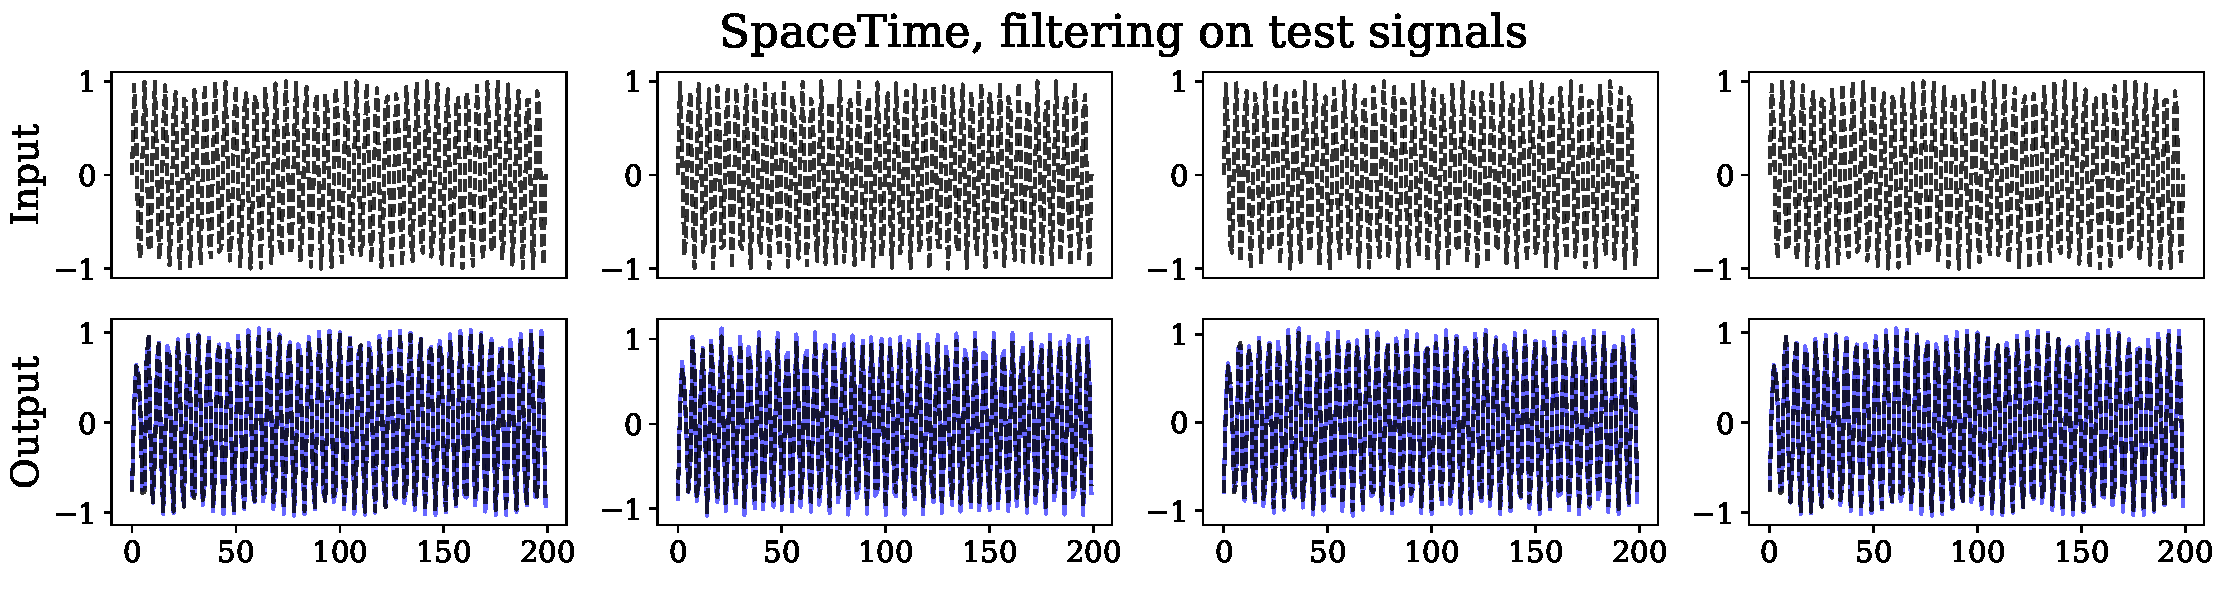
\includegraphics[scale=0.35]{_ICLR2023_paper/figures/dsp_SpaceTime.pdf}
    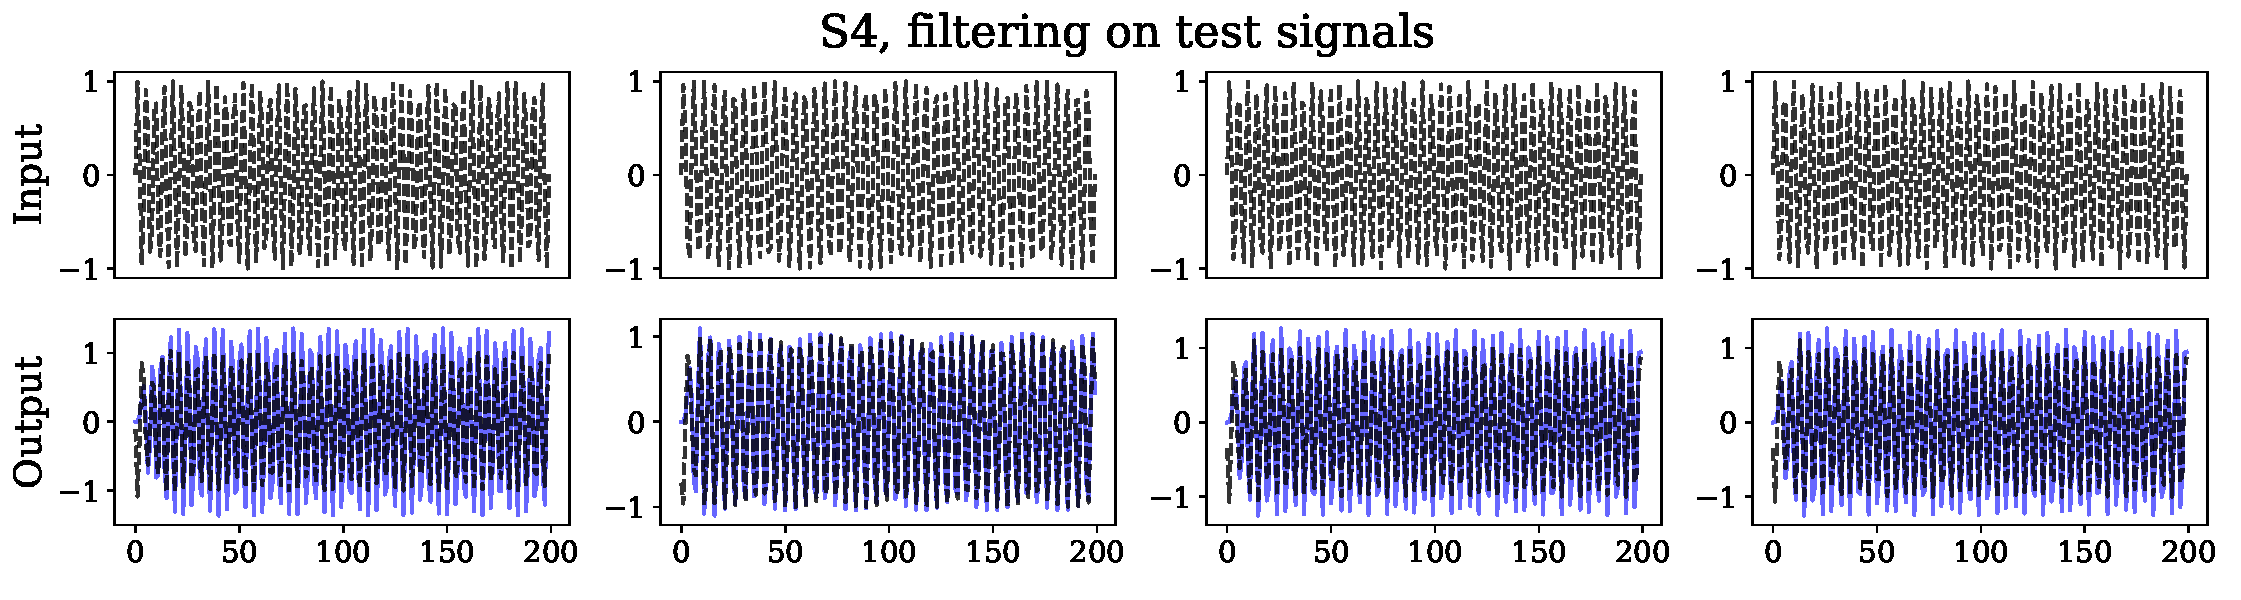
\includegraphics[scale=0.35]{_ICLR2023_paper/figures/dsp_S4.pdf}
    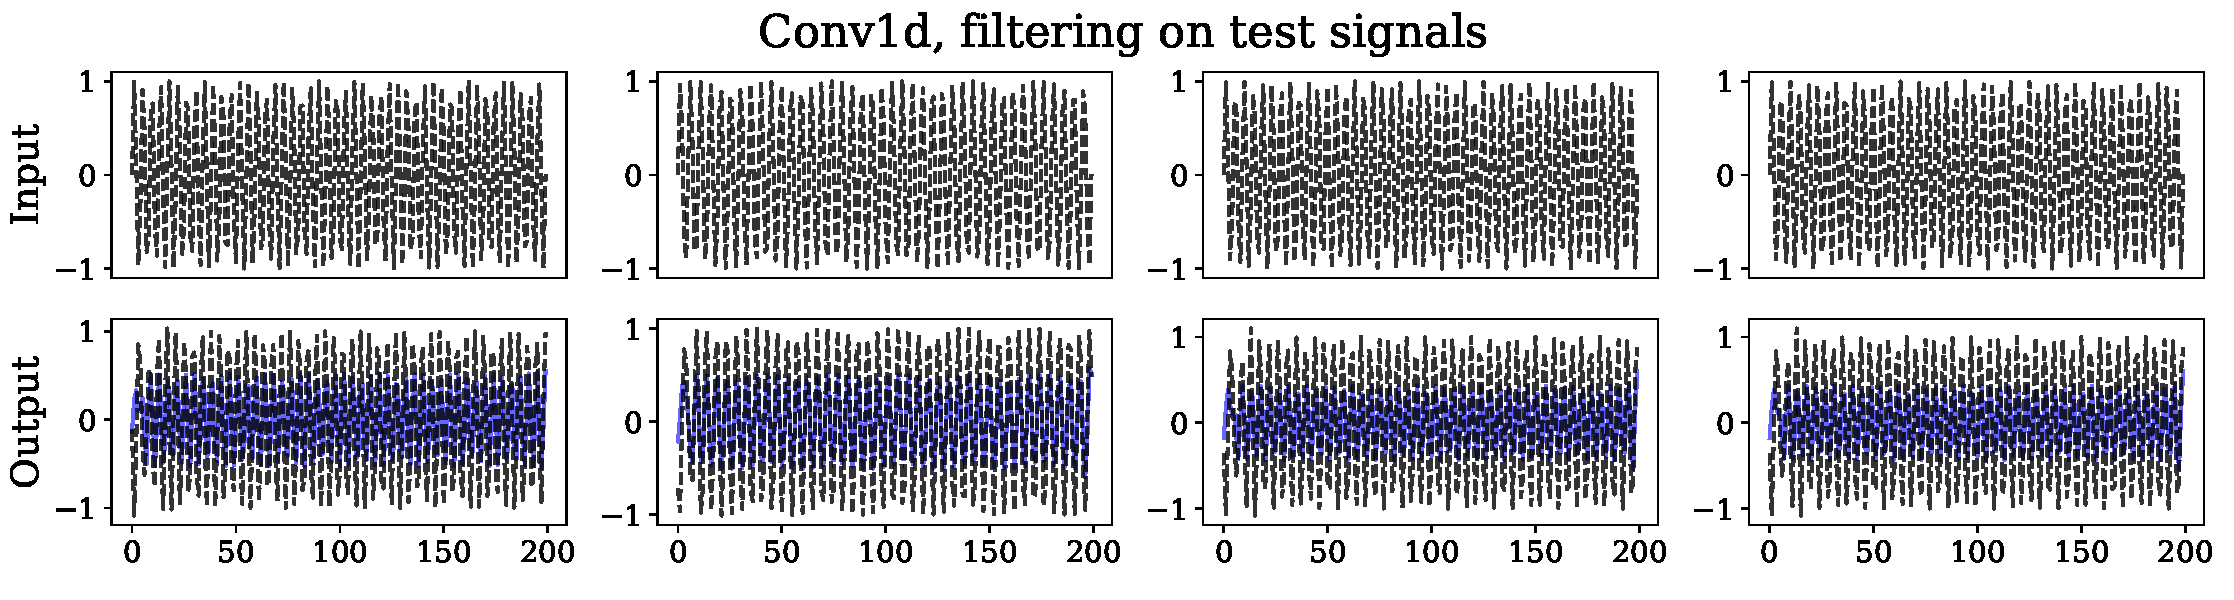
\includegraphics[scale=0.35]{_ICLR2023_paper/figures/dsp_Conv1d.pdf}
    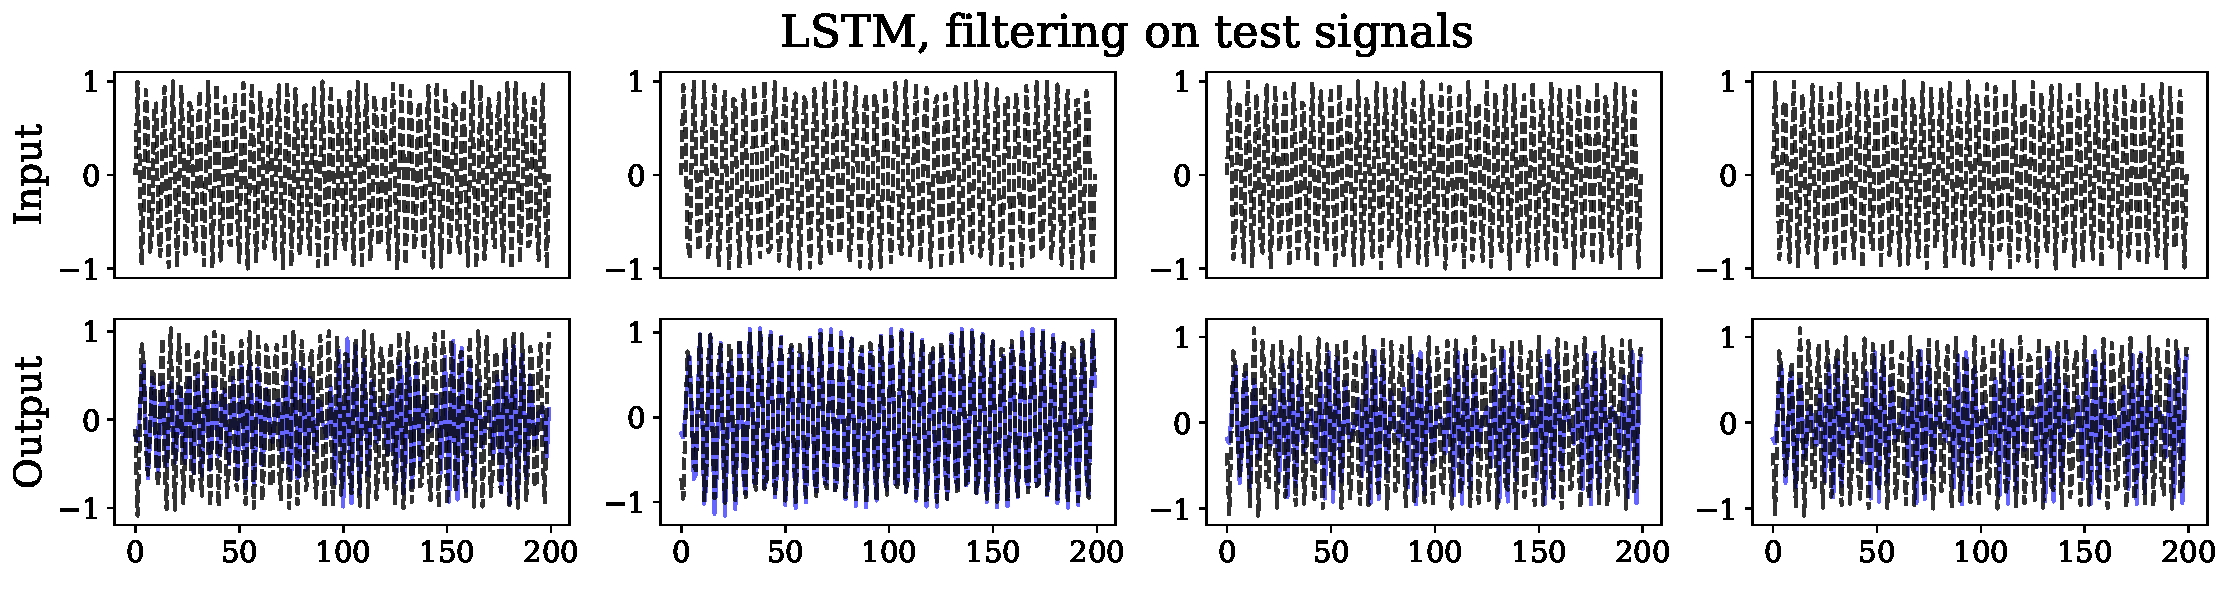
\includegraphics[scale=0.35]{_ICLR2023_paper/figures/dsp_LSTM.pdf}
    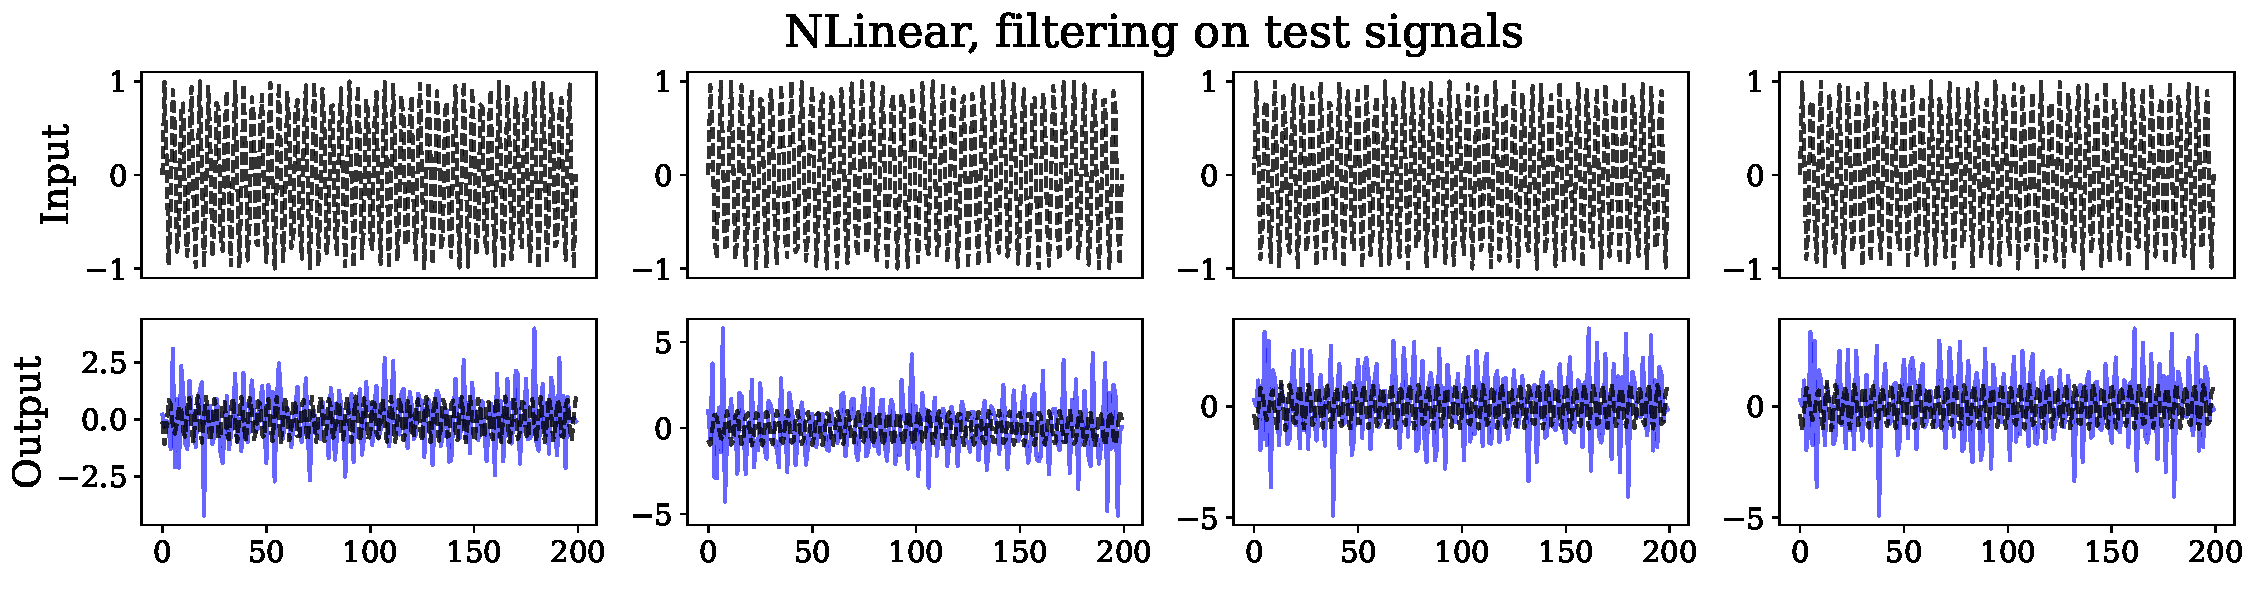
\includegraphics[scale=0.35]{_ICLR2023_paper/figures/dsp_NLinear.pdf}
    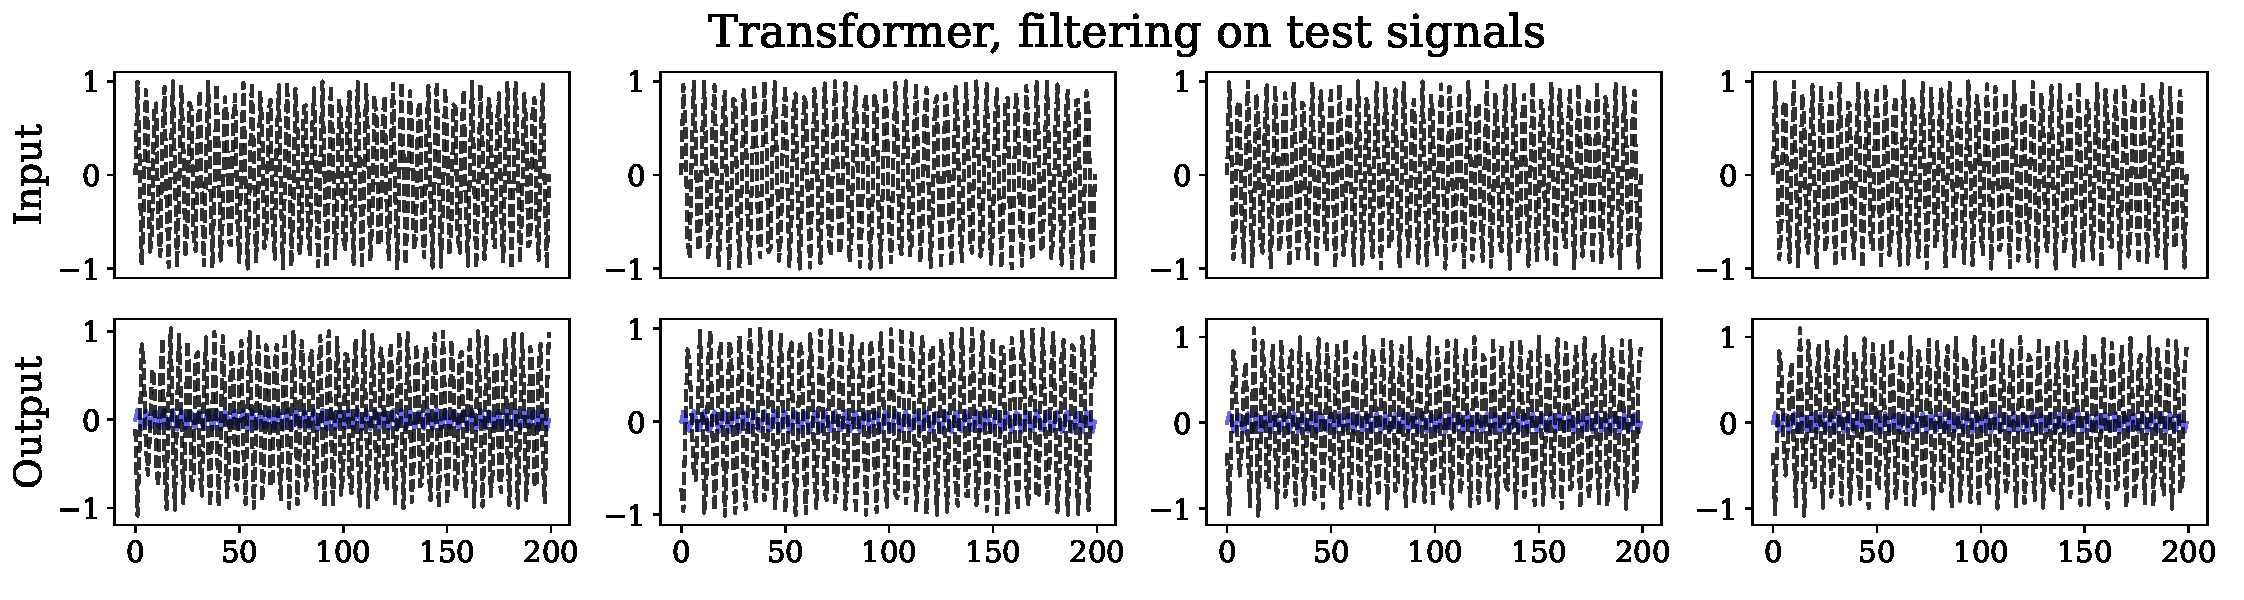
\includegraphics[scale=0.35]{_ICLR2023_paper/figures/dsp_Transformer.pdf}
    \caption{Testing the capability of different sequence--to--sequence models to approximate the input--output map of digital filters. In blue, we show the output signal filtered by each model. The ground--truth digital filter is a Butterworth of order $10$.}
    \label{fig:dsp_synthetic}
\end{figure}
%





\begin{sidewaystable}[h]
    \tiny
    \centering
    \caption{Monash forecasting. Test RMSE of \ourmethod for each dataset (best result selected via validation RMSE, average of $3$ runs).}
    \label{tab:monash}
    \begin{tabular}{c|c|cccccc|ccccc}
    \toprule
    %
    Dataset  & \ourmethod & SES & Theta & TBATS & ETS & (DHR-)ARIMA & PR & CatBoost & DeepAR & N-BEATS & WaveNet & Transformer \\
    %
    \midrule
    M1 Yearly & \underline{135508.3} & 193829.5 & 171458.1 & \textbf{116850.9} & 167739.0 & 175343.8 & 152038.7 & 237644.5 & 173075.1 & 192489.8 & 312821.8 & 182850.6 \\
    
    M1 Quarterly & \underline{2200.3} & 2545.7&	2282.7	&2673.9&	2408.5&	2538.5&	1909.3&	2161.0& 2313.3&	2267.3&	2271.7&	2231.5  \\    
    
    M1 Monthly & 2601.1 & 2725.8 & 2564.9 & 2594.5 & 2264.0 & 2450.6 & 2478.8 & 2461.7 & 2202.2 & \textbf{2183.4} & 2578.9 & 3129.8  \\

    M3 Yearly & 1412.4 & 1172.9&	1106.1&	1386.3	&1189.2	&1662.2	&1181.8&	1341.7&		1157.9&	1117.4&	1147.6&	1084.8 \\
    
    M3 Quarterly & 676.1 & 670.6&	567.7&	653.6&	598.7&	650.8&	605.5&	698.0&	606.6&	582.8&	606.8&	819.2\\ 
    
    M3 Monthly & 897.12 & 893.9	&754.0&	765.2	&755.3&	790.8&	830.0&	874.2&	873.7&	796.9&	845.3&	948.4 \\
    
    M3 Other & 265.56 & 309.7	&242.1&	217.0&	224.1	&220.8	&262.3&	349.9&	277.7&	248.5&	277.0	&271.0 \\
    
    M4 Quarterly & 718.2 & 732.8&	673.2&	672.7&	674.3&	710.0&	711.9&	714.2&	700.3&	684.7&	697.0&	739.1 \\
    
    M4 Monthly & 1092.2 & 755.5	&683.7&	743.4&	705.7&	702.1&	720.5&	734.8&	740.3&	705.2&	787.9&	902.4\\ 
    
    M4 Weekly & \textbf{348.3}& 412.6	&405.2&	356.7&	408.5	&386.3&	350.3&	420.8&	422.2&	330.8&	437.3&	456.9\\ 
    
    M4 Daily &\textbf{183.2}& 209.8&	210.4&	\underline{208.4}&	230.0	&212.6&	213.0&	263.1	&343.5&	221.7&	220.5&	233.6\\ 
    
    M4 Hourly & \textbf{255.2} & 1476.8	&1483.7	&469.9&	3830.4&	1563.1&	\underline{313.0} &	344.6&	1095.1&	501.2&	468.1&	391.2\\
    
    Tourism Yearly & \textbf{74799.2}& 106665.2&	99914.2&	105799.4&	104700.5&	106082.6&	89645.6	&87489.0&	78470.7&	78241.7	&77581.3&	80089.3\\
    
    Tourism Quarterly & 11608.32& 15000.0&	9254.6&	12001.5	&10812.3	&12564.8	&11746.9	&12788.0	&11762.0&	11306.0	&11546.6	&11724.1 \\
    
    Tourism Monthly & 3181.2& 7039.4&	2702.0	&3661.5	&2543.0	&3132.4&	2739.4&	3102.8&	2359.9&	2596.2&	2694.2&	2660.1\\
    
    Pedestrian & 69.6& 228.1&	228.2	&261.3&	278.3&	820.3&	61.8&	60.8&	65.8&	99.3&	68.0&	70.2\\
    
    Weather & \textbf{2.7}& 2.9	&3.3&	2.9&	3.0&	3.1	&9.1&	3.1&	\textbf{2.7}	&3.1&	3.0	&2.8\\
    
    NN5 Weekly & \textbf{16.9}& 18.8&	18.7&	18.5&	18.8&	18.6&	18.6&	18.7&	18.5&	17.4&	24.2&	24.0 \\
    
    Solar $10$ min &7.4& 7.2&	7.2	&10.7&	7.2	&5.6&	7.2	&8.7&	7.2	&6.6&	8.0&	7.2\\
    
    Solar Weekly &1423.7& 1331.3&	1341.6&	1049.0&	1264.4&	967.9&	1168.2&	1754.2&	873.6&	1307.8&	2569.3&	693.8\\
    
    Electricity Hourly & \textbf{475.1} & 1026.3&	1026.4&	743.4&	1524.9&	1082.4&	689.9&	582.7&	\underline{478.0} &	510.9&	489.9&	514.7\\
    
    Electricity Weekly &37802.2& 77067.9&	76935.6&	28039.7	&70369.0&	32594.8&	47802.1&	37289.7	&53100.3&	35576.8	&63916.9&	78894.7\\
    
    Fred-MD &3743.6& 3103.0&	3898.7&	2295.7&	2341.7	&3312.5&	9736.9&	2679.4&	4638.7&	2813.0&	2779.5&	5098.9\\
    
    Traffic Hourly &0.03& 0.04&	0.04	&0.05&	0.04	&0.04&	0.03	&0.03&	0.02&	0.02	&0.03&	0.02\\
    
    Traffic Weekly &\textbf{1.3}& 1.5&	1.5	&1.5&	1.5	&1.5&	1.5&	1.5	&1.5&	1.4	&1.6&	1.9\\
    
    Hospital &40.1& 26.6&	22.6&	21.3&	22.0	&23.7&	23.5&	23.5&	22.0&	24.2&	23.4&	40.5\\
    
    Covid &490.1& 403.4&	370.1&	113.0&	102.1&	100.5&	394.1&	607.9&	230.5&	186.5&	1135.4&	480.0\\
    
    Saugeen & \textbf{24.0} & 39.8	&39.8	&42.6&	50.4&	43.2&	47.7&	\underline{39.3} &	45.3&	48.9&	43.0&	49.1\\
    
    US Births &630.2& 1369.5&	735.5&	606.5&	607.2&	705.5&	732.1&	618.4&	684.0&	627.7&	768.8&	686.5\\
    
    Sunspot &3.1& 5.0	&5.0&	3.0	&5.0&	3.0	&4.0&	2.4	&1.1&	14.5&	0.7	&0.5\\
    
    Car Parts & 0.64 & 0.71&	0.65	&0.71&	0.71&	0.71&	\underline{0.58}&	0.71&	\textbf{0.50}&	1.0&	\underline{0.58}&	0.5\\
    
    Vehicle Trips &30.4& 36.5&	37.4&	25.7&	37.6&	35.0&	31.7&	27.3&	26.5&	33.6&	29.0&	33.0\\
    \bottomrule
    %
    \end{tabular}
\end{sidewaystable}

%
\end{document}